%%%%%%%%%%%%%%%%%%%%%%%%%%%%%%%%%%%%%%%%%%%%%%%%%%%%%%%%%%%%%%%%%%%%%
%
% Complete documentation on the extended LaTeX markup used for Insight
% documentation is available in ``Documenting Insight'', that is part
% of the standard documentation for Insight.  It may be found online
% at:
%
%                    http://www.itk.org
%
%%%%%%%%%%%%%%%%%%%%%%%%%%%%%%%%%%%%%%%%%%%%%%%%%%%%%%%%%%%%%%%%%%%%%

\documentclass{InsightSoftwareGuide}


\usepackage[dvips]{graphicx}
\usepackage{times}


%%% \usepackage[latin1]{inputenc}
%%% \selectlanguage{french}
% Configuration pour les accents francais pour l'OTB
\usepackage[latin1]{inputenc}
%\usepackage[french]{babel}



\newif\ifitkFullVersion
\itkFullVersiontrue
%\itkFullVersionfalse

\newif\ifitkPrintedVersion
\itkPrintedVersiontrue
%\itkPrintedVersionfalse


%%%%%%%%%%%%%%%%%%%%%%%%%%%%%%%%%%%%%%%%%%%%%%%%%%%%%%%%%%%%%%%%%%
%
%  hyperref should be the last package to be loaded.
%
%%%%%%%%%%%%%%%%%%%%%%%%%%%%%%%%%%%%%%%%%%%%%%%%%%%%%%%%%%%%%%%%%%
\ifitkPrintedVersion
\usepackage[dvips,
pdftitle={OTB Software Guide},
pdfauthor={CNES},
pdfsubject={Remote Sensing, Orfeo, Pleiades, Cosmo Skymed},
pdfkeywords={mage processing, Remote sensing, Guide},
pdfpagemode={UseOutlines},
bookmarks,bookmarksopen,
pdfstartview={FitH},
backref,
colorlinks,linkcolor={black},citecolor={black},urlcolor={black},
]{hyperref}
\else
\usepackage[dvips,
pdftitle={OTB Software Guide},
pdfauthor={CNES},
pdfsubject={Remote Sensing, Orfeo, Pleiades, Cosmo Skymed},
pdfkeywords={mage processing, Remote sensing, Guide},
pdfpagemode={UseOutlines},
bookmarks,bookmarksopen,
pdfstartview={FitH},
backref,
colorlinks,linkcolor={blue},citecolor={blue},urlcolor={blue},
]{hyperref}
\fi

\usepackage{amsmath,amssymb,amsfonts}
%%%%%%%%%%%%%%%%%%%%%%%%%%%%%%%%%%%%%%%%%%%%%%%%%%%%%%%%%%%%%%%%%%%
%
%
%   Load configuration parameters prepared by CMake
%
%
%%%%%%%%%%%%%%%%%%%%%%%%%%%%%%%%%%%%%%%%%%%%%%%%%%%%%%%%%%%%%%%%%%%

% Define where in the disk is the Insight source tree 
% \def\ITKSOURCEDIR{}
% THOMAS
\def\ITKSOURCEDIR{/ORFEO/thomas/ORFEO-TOOLBOX/otb/OTB}
\graphicspath{{/ORFEO/thomas/ORFEO-TOOLBOX/otb/OTB-Documents/SoftwareGuide/Art/}{/ORFEO/thomas/ORFEO-TOOLBOX/otb/OTB-Documents/SoftwareGuide/Art/}}
\def\bibtexdatabasepath{/ORFEO/thomas/ORFEO-TOOLBOX/otb/OTB-Documents/SoftwareGuide/../Latex/Insight}


% Define command to make reference to on-line Doxygen documentation
\newcommand{\doxygen}[1]{
\href{http://www.itk.org/Doxygen/html/classitk_1_1#1.html}{\code{itk::#1}}}  

% Define command to make reference to on-line Doxygen documentation
\newcommand{\subdoxygen}[2]{
\href{http://www.itk.org/Doxygen/html/classitk_1_1#1_1_1#2.html}{\code{itk::#1::#2}}}  

% Define command for the standard comment introducing classes with similar functionalities
\newcommand{\relatedClasses}{
\textbf{The following classes provide similar functionality:}}


\def\logoCNES{CNES_nom.eps}
%%%%%%%%%%%%%%%%%%%%%%%%%%%%%%%%%%%%%%%%%%%%%%%%%%%%%%%%%%%%%%%%%%%
%
%
%           The Insight Toolkit Software Guide
%
%
%%%%%%%%%%%%%%%%%%%%%%%%%%%%%%%%%%%%%%%%%%%%%%%%%%%%%%%%%%%%%%%%%%%

\title{The ORFEO Tool Box Software Guide\\ Second Edition\\ Updated
  for OTB-1.0.1}

\author{OTB Development Team}

\authoraddress{
  \url{http://smsc.cnes.fr/PLEIADES/A_prog_accomp.htm}\\
  Email: \email{jordi.inglada@cnes.fr}
}

\date{\today}


% actually write the .idx file
\makeindex

\setcounter{tocdepth}{3}



%%%%%%%%%%%%%%%%%%%%%%%%%%%%%%%%%%%%%%%%%%%%%%%%%%%%%%%%%%%%%%%%%%%
%
%           Begin Document
%
%%%%%%%%%%%%%%%%%%%%%%%%%%%%%%%%%%%%%%%%%%%%%%%%%%%%%%%%%%%%%%%%%%%

\begin{document}

\ifitkPrintedVersion
%% 
\begin{minipage}[t][3cm][b]{\textwidth}
\rule{14cm}{1pt}
\end{minipage}


\begin{minipage}[t][3cm][b]{\textwidth}
\Huge
The ITK Software Guide\\
\normalsize
\par
\emph{updated for version 2.4}\\
\end{minipage}

\hfill
\begin{minipage}[t][6cm][b]{0.6\textwidth}
\Large
\renewcommand{\baselinestretch}{1.5}
Luis Ib\'{a}\~{n}ez\\
Will Schroeder\\
Lydia Ng\\
Josh Cates\\
and the \emph{Insight Software Consortium}
\normalsize
\end{minipage}


\begin{minipage}[t][2cm][b]{\textwidth}
\rule{14cm}{1pt}
\end{minipage}

\newpage

\begin{minipage}[t][4cm][b]{\textwidth}
\begin{center}

\includegraphics[width=0.5\textwidth]{Kitware-logo-medium-res.eps}
\end{center}
\par
\begin{center}
\large
\copyright 2003 Kitware, Inc. \emph{(cover, preface, postface)}\\
\copyright 2003 Insight Software Consortium \emph{(main text body)}\\
Published by Kitware, Inc. \texttt{http://www.kitware.com}
\normalsize
\end{center}
\end{minipage}


\begin{minipage}[t][2.25cm][b]{\textwidth}
\begin{center}
All rights reserved. No part of this book may be reproduced, in any form 
or by any means, without the express written permission of the copyright
holders. An electronic version of this document is available from
\texttt{http://www.itk.org} and may be used under the provisions of the
ITK copyright found at \texttt{http://www.itk.org/HTML/Copyright.htm}.
\end{center}
\end{minipage}


\begin{minipage}[t][3.2cm][b]{\textwidth}
\begin{center}
The publisher Kitware, Inc. offers discounts on this book when ordered in
bulk quantities.\\
The publisher also produces companion works to this text such as \emph{The
Visualization Toolkit An Object-Oriented Approach to 3D Graphics 3rd Edition}
by Schroeder, Martin and Lorensen, \emph{Mastering CMake} by Martin and
Hoffman and \emph{The VTK's Users Guide} by Kitware.\\
For more information contact Kitware, Inc at \texttt{kitware@kitware.com}.\\
You may also order directly from Kitware's electronic store at
\texttt{http://www.kitware.com/products}\\
\end{center}
\end{minipage}

\begin{minipage}[t][2.7cm][b]{\textwidth}
\begin{center}
Contributors to this work include those listed on the title page as well
as:\\ Cover Design: Luis Ib\'{a}\~{n}ez and S\'{e}bastien Barr\'{e}\\
Technical Contributors: World-Wide ITK Developer Community at
\texttt{www.itk.org}. \\Document created with \LaTeX{}, using CMake as
configuration manager, with a Perl script to extract examples from the
\code{Insight/Examples} directory. All code in this document compiled at
the time of publication.
\end{center}
\end{minipage}


\begin{minipage}[t][2.5cm][b]{\textwidth}
\begin{center}
This project has been funded in whole or in part with Federal funds from the
National Institutes of Health (NLM, NIDCR, NIMH, NEI, NINDS, NIDCD, NCI), the
NSF, and the DoD (TATRC) under the direction of the National Library of
Medicine, National Institutes of Health, contracts number N01-LM-9-3531,
N01-LM-9-3532, N01-LM-0-3501, N01-LM-0-3502, N01-LM-0-3503, and
N01-LM-0-3504.
\end{center}
\end{minipage}


\begin{minipage}[t][1.0cm][b]{\textwidth}
\begin{center}
All product names mentioned herein are the trademarks of their respective 
owners.
\end{center}
\end{minipage}


\begin{minipage}[t][1.0cm][b]{\textwidth}
\begin{center}
Printed and produced in the United States of America.\\
ISBN 1-930934-15-7
\end{center}
\end{minipage}

\fi

\maketitle

\frontmatter

\hyperbaseurl{http://smsc.cnes.fr/PLEIADES/A_prog_accomp.htm}



%%%%%%%%%%%%%%%%%%%%%%%%%%%%%%%%%%%%%%%%%%
%
%  Page with Quote and ITK Logo
%
%%%%%%%%%%%%%%%%%%%%%%%%%%%%%%%%%%%%%%%%%%
\cleardoublepage

%\begin{minipage}[t][10cm][b]{\textwidth}
%\center
%\includegraphics[width=0.5\textwidth]{otbLogo.eps}
%\large
%\begin{center}
%\emph{The purpose of computing is Insight, not numbers.}\\
%\end{center}
%\hspace{8cm} Richard Hamming
%\normalsize
%\end{minipage}



%%%%%%%%%%%%%%%%%%%%%%%%%%%%%%%%%%%%%%%%%%%%%%
%
% remove headings from the following material
\pagestyle{plain}
%
%%%%%%%%%%%%%%%%%%%%%%%%%%%%%%%%%%%%%%%%%%%%%%



%%\ifitkPrintedVersion 
%% % We want this material to fit on two pages
\small

\chapter*{About the Cover}

Creating the cover image demonstrating the capabilities of the toolkit was a
challenging task.\footnote{The source code for the cover is available from
InsightDocuments/SoftwareGuide/Cover/Source/.} Given that the origins of ITK
are with the Visible Human Project it seemed appropriate to create an image
utilizing the VHP data sets, and it was decided to use the more recently
acquired Visible Woman dataset.  Both the RGB cryosections and the CT scans
were combined in the same scene.

\begin{description}

\item [Removing the Gel.]
The body of the Visible Woman was immersed in a block of gel during the
freezing process. This gel appears as a blue material in the cryogenic data.
To remove the gel, the joint histogram of RGB values was computed. This
resulted in an 3D image of $256\times256\times256$ pixels. The histogram
image was visualized in VolView.\footnote{VolView is a commercial product
from Kitware. It supports ITK plug-ins and is available as a free viewer or
may be licensed with advanced functionality. See
http://www.kitware.com/products/volview.html for information.} The cluster
corresponding to the statistical distribution of blue values was identified
visually, and a separating plane was manually defined in RGB space. The
equation of this plane was subsequently used to discriminate pixels in the
gel from pixels in the anatomical structures. The gel pixels were zeroed out
and the RGB values on the body were preserved.

\item[The Skin.]
The skin was easy to segment once the gel was removed. A simple region
growing algorithm was used requiring seed points in the region previously
occupied by the gel and then set to zero values. An anti-aliasing filter was
applied in order to generate an image of pixel type float where the surface
was represented by the zero set. This data set was exported to VTK where a
contouring filter was used to extract the surface and introduce it in the VTK
visualization pipeline.

\item[The Brain.]
The visible part of the brain represents the surface of the gray matter.  The
brain was segmented using the vector version of the confidence connected
image filter.  This filter implements a region growing algorithm that starts
from a set of seed points and adds neighboring pixels subject to a condition
of homogeneity.

The set of sparse points obtained from the region growing algorithm was
passed through a mathematical morphology dilation in order to close holes and
then through a binary median filter. The binary median filter has the
outstanding characteristic of being very simple in implementation by applying
a sophisticated effect on the image. Qualitatively it is equivalent to a
curvature flow evolution of the iso-contours. In fact the binary median
filter as implemented in ITK is equivalent to the majority filter that
belongs to the family of voting filters classified as a subset of the
\emph{Larger than Life} cellular automata. Finally, the volume resulting from
the median filter was passed through the anti-aliasing image filter. As
before, VTK was used to extract the surface.

\item[The Neck Musculature.]
The neck musculature was not perfectly segmented. Indeed, the resulting
surface is a fusion of muscles, blood vessels and other anatomical
structures. The segmentation was performed by applying the
VectorConfidenceConnectedImageFilter to the cryogenic dataset. Approximately
60 seed points were manually selected and then passed to the filter as
input. The binary mask produced by the filter was dilated with a mathematical
morphology filter and smoothed with the BinaryMedianImageFilter. The
AntiAliasBinaryImageFilter was used at the end to reduce the pixelization
effects prior to the extraction of the iso-surface with vtkContourFilter.

\item[The Skull.]
The skull was segmented from the CT data set and registered to the cryogenic
data. The segmentation was performed by simple thresholding, which was good
enough for the cover image. As a result, most of the bone structures are
actually fused together. This includes the jaw bone and the cervical
vertebrae.

\item[The Eye.] 
The eye is charged with symbolism in this image. This is due in part because
the motivation for the toolkit is the analysis of the Visible Human data,
and in part because the name of the toolkit is \emph{Insight}.

The first step in processing the eye was to extract a sub-image of
$60\times60\times60$ pixels centered around the eyeball from the RGB
cryogenic data set. This small volume was then processed with the vector
gradient anisotropic diffusion filter in order to increase the homogeneity of
the pixels in the eyeball.

The smoothed volume was segmented using the
VectorConfidenceConnectedImageFilter using 10 seed points. The resulting
binary mask was dilated with a mathematical morphology filter with a
structuring element of radius one, then smoothed with a binary mean image
filter (equivalent to majority voting cellular automata). Finally the mask
was processed with the AntiAliasBinaryImageFilter in order to generate a
float image with the eyeball contour embedded as a zero set.

\item[Visualization.]
The visualization of the segmentation was done by passing all the binary
masks through the AntiAliasBinaryImageFilter, generating iso-contours with
VTK filters, and then setting up a VTK Tcl script. The skin surface was
clipped using the vtkClipPolyDataFilter using the implicit function
vtkCylinder. The vtkWindowToImageFilter proved to be quite useful for
generating the final high resolution rendering of the scene ($3000\times3000$
pixels).

\item[Cosmetic Postprocessing.]
We have to confess that we used Adobe Photoshop to post-process the image. In
particular, the background of the image was adjusted using Photoshop's color
selection. The overall composition of the image with the cover text and
graphics was also performed using Photoshop.

\end{description}

\normalsize

%%\fi

\chapter*{Foreword}
\noindent


Beside the Pleiades (PHR) and Cosmo-Skymed (CSK) systems developments
forming ORFEO, the dual and bilateral system (France - Italy) for
Earth Observation, the ORFEO Accompaniment Program was set up, to
prepare, accompany and promote the use and the exploitation of the
images derived from these sensors.

The creation of a preparatory
program\footnote{http://smsc.cnes.fr/PLEIADES/A\_prog\_accomp.htm} is
needed because of:
\begin{itemize}
\item the new capabilities and performances of the ORFEO systems
  (optical and radar high resolution, access capability, data quality,
  possibility to acquire simultaneously in optic and radar),
\item the implied need of new methodological developments : new
  processing methods, or adaptation of existing methods,
\item the need to realise those new developments in very close
  cooperation with the final users for better integration of new
  products in their systems.

\end{itemize}

This program was initiated by CNES mid-2003 and will last until mid
2013.  It consists in two parts, between which it is necessary to keep
a strong interaction:
\begin{itemize}
\item A Thematic part,
\item A Methodological part.
\end{itemize}

The Thematic part covers a large range of applications (civil and
defence), and aims at specifying and validating value added products
and services required by end users. This part includes consideration
about products integration in the operational systems or processing
chains. It also includes a careful thought on intermediary structures
to be developed to help non-autonomous users. Lastly, this part aims
at raising future users awareness, through practical demonstrations
and validations.

The Methodological part objective is the definition and the
development of tools for the operational exploitation of the
submetric optic and radar images (tridimensional aspects, changes
detection, texture analysis, pattern matching, optic radar
complementarities). It is mainly based on R\&D studies and doctorate
and post-doctorate researches.

In this context, CNES\footnote{http://www.cnes.fr} decided to develop
the \emph{ORFEO ToolBox} (OTB), a set of algorithms encapsulated in a
software library. The goals of the OTB is to capitalise a methological
\textit{savoir faire} in order to adopt an incremental development
approach aiming to efficiently exploit the results obtained in the
frame of methodological R\&D studies.

All the developments are based on FLOSS (Free/Libre Open Source
Software) or existing CNES developments. OTB is distributed under the
C\'eCILL licence,
\url{http://www.cecill.info/licences/Licence_CeCILL_V2-en.html}.

OTB is implemented in C++ and is mainly based on
ITK\footnote{http://www.itk.org} (Insight Toolkit).


%% L'environnement de l'OTB est mis en place par l'outil CMake\footnote{http://www.cmake.org},
%% permettant ainsi de g\'{e}rer les proc\'{e}dures de compilation, g\'{e}n\'{e}ration et d'installation et ce quelque sois la plate forme cible.

%% Dans un souci d'homog\'{e}n\'{e}isation, l'OTB est con\c{c}ue et d\'{e}velopp\'{e}e suivant la philosophie et les principes \'{e}dict\'{e}s
%% par la biblioth\`{e}que ITK (programmation g\'{e}n\'{e}rique, m\'{e}canisme des \emph{Object Factories}, \emph{Smart pointers}, exceptions, \emph{Multi-Threading}, etc...).
%% Ces principes sont pr\'{e}sent\'{e}s dans le paragraphe \emph{3.2 Essential System Concepts} du guide ITK \url{http://www.itk.org/ItkSoftwareGuide.pdf}

%% Enfin, la m\'{e}thodologie de d\'{e}veloppement appliqu\'{e}e s'appuie sur une approche it\'{e}rative bas\'{e}e sur la programmation agile :
%% le sch\'{e}ma de d\'{e}veloppement suit le cycle \'{e}dict\'{e}e par la m\'{e}thodolgie de l'eXtreme Programming (XP)\footnote{http://www.xprogramming.com}.



%% Ce document constitue le guide d'utilisation et de d\'{e}veloppement de l'OTB. La version la plus r\'{e}cente de ce document est accessible \`{a}
%% \url{http://smsc.cnes.fr/PLEIADES/Fr/A_prog_accomp.htm/OTB/otbSoftwareGuide.pdf}.



\chapter*{Contributors}
\noindent

The ORFEO Toolbox is a project conducted by CNES and developed in
cooperation with CS (Communication \& Syst\`{e}mes), \url{http://www.c-s.fr}.\\

This Software Guide is based on the ITK Software Guide: the build
process for the documentation, many examples and even the \LaTeX~ ~
sources were taken from ITK. We are very grateful to the ITK
developpers and contributors and especially to Luis Ib\'a\~nez.\\

The OTB specifics were implemented and documented by the OTB Development Team with some help from several contributors, without these people\footnote{list had been generated at random without any hierarchy or amount of contribution consideration}, OTB will not be where it is today:

Gwendoline Blanchet (CNES), Manuel Grizonnet (CNES), Antonio Valentino, Vincent Poulain (CNES), Yannick Reynard, Edouard Barthelet (Telecom Bretagne and Thales Communications), Julien Malik (CS), Jan Wegner, Michael Seymour (EADS), Massimo Di Stefano, Jordi Inglada (CNES), Mathieu Deltorre (CS), Jean-Guilhem Cailton (Ark\'emie), Emmanuel Christophe (CNES, then CRISP, then Google), David Dubois, Cyrille Valladeau (CS), Romain Garrigues (CS), Eric Bughin (CMLA), Aik Song Chia (CRISP), Otmane Lahlou (CS), Vincent Schut (Sarvision), S\'ebastien Dinot (CS), Guillaume Borrut (CS), Patrick Imbo (CS), Miarintsoa Ramanantsimiavona, Conrad Bielski (JRC), Caroline Ruffel (CS), Julien Osman, Amit Kulkarni, Tishampati Dhar, Etienne Bougoin (CS), Adamo Ferro, Julien Michel (CS then CNES), Aur\'elien Bricier (CS), Thomas Feuvrier (CS), Stephane May (CNES), Gr\'egoire Mercier (Telecom Bretagne), Rik Bellens, Christophe Lay, Angelos Tzotsos

Contributions from users are expected and encouraged for the comming
versions of OTB.





%%%%%%%%%%%%%%%%%%%%%%%%%%%%%%%%%%%%%%%%%%%%%%%%%%%%%%%%%
%
% Insert Table of Contents; List of Figures and Tables
%
%%%%%%%%%%%%%%%%%%%%%%%%%%%%%%%%%%%%%%%%%%%%%%%%%%%%%%%%%


%%%%%%%%%%%%%%%%%%%%%%%%%%%%%%%%%%%%%%%%%%%%%%
%
% enable headings from the following material
\pagestyle{normal}
%
%%%%%%%%%%%%%%%%%%%%%%%%%%%%%%%%%%%%%%%%%%%%%%
\small
\tableofcontents
\listoffigures
\listoftables
\normalsize




%%%%%%%%%%%%%%%%%%%%%%%%%%%%%%%%%%%%%%%%%
% 
% Begin technical content
% 
%%%%%%%%%%%%%%%%%%%%%%%%%%%%%%%%%%%%%%%%%

\mainmatter

\part{Introduction}

\chapter{Welcome}
\label{chapter:Welcome}

Welcome to the \emph{ORFEO ToolBox (OTB) Software Guide}.

This document presents the essential concepts used in OTB. It will
guide you through the road of learning and using OTB. The Doxygen
documentation for the OTB application programming interface is
available on line at \url{http://smsc.cnes.fr/PLEIADES/OTB/Doxygen/html}.

\section{Organization}
\label{sec:Organization}

This software guide is divided into three parts, each of which is further
divided into several chapters. Part I is a general introduction to OTB,
with---in the next chapter---a description of how to install the ORFEO
Toolbox on your computer. Part I also
introduces basic system concepts such as an overview of the system
architecture, and how to build applications in the C++ programming
language. Part II describes the system from the user point of view. Dozens
of examples are used to illustrate important system features. Part III is for
the OTB developer. It explains how to create your own classes and extend
the system.%, and interface to windowing and GUI systems.

\section{How to Learn OTB}
\label{sec:HowToLearnOTB}

There are two broad categories of users of OTB. First are class
developers, those who create classes in C++. The second, users, employ
existing C++ classes to build applications. Class developers must be
proficient in C++, and if they are extending or modifying OTB, they
must also be familiar with OTB's internal structures and design
(material covered in Part III). 

The key to learning how to use OTB is to become familiar with its
palette of objects and the ways of combining them. We recommend that you learn the system by studying the
examples and then, if you are a class developer, study the source
code. Start by reading Chapter \ref{chapter:SystemOverview}, which provides an overview of some
of the key concepts in the system, and then review the examples in
Part II. You may also wish to compile and run the dozens of examples
distributed with the source code found in the directory
\code{OTB/Examples}. (Please see the file
\code{OTB/Examples/README.txt} for a description of the examples
contained in the various subdirectories.) There are also several
hundreds of tests found in the source distribution in
\code{OTB/Testing/Code}, most of which are minimally documented
testing code. However, they may be useful to see how classes are used
together in OTB, especially since they are designed to exercise as
much of the functionality of each class as possible.

\section{Software Organization}
\label{sec:SoftwareOrganization}

The following sections describe the directory contents, summarize the
software functionality in each directory, and locate the documentation and
data.

\subsection{Obtaining the Software}
\label{sec:ObtainingTheSoftware}

Periodic releases of the software are available on the OTB Web
site. These official releases are available a few times a year and
announced on the ORFEO Web pages and mailing lists. 

This software guide assumes that you are working with the official OTB
version 1.0 release (available on the OTB Web site). %If you are a new user,
%we highly recommend that you use the released version of the software.

\section{Downloading OTB}
\label{sec:DownloadingOTB}
 
\index{Downloading}

OTB can be downloaded without cost from the following web site:
\begin{center} 
  \url{http://smsc.cnes.fr/PLEIADES/A_prog_accomp.htm}
\end{center}
In order to track the kind of applications for which OTB is being used, you
will be asked to complete a form prior to downloading the software.
The information you provide in this form will help developers to get a better
idea of the interests and skills of the toolkit users.

Once you fill out this form you will have access to the download
page. This page can be book marked to facilitate subsequent visits to
the download site without having to complete any form again.

 Then choose the tarball that better fits your system. The options
are \code{.zip} and \code{.tgz} files.  The first type is better suited for
MS-Windows while the second one is the preferred format for UNIX systems.

Once you unzip or untar the file, a directory called \code{OTB} will be
created in your disk and you will be ready for starting the configuration
process described in Section \ref{sec:CMakeforOTB} on page 
\pageref{sec:CMakeforOTB}.


\subsection{Join the Mailing List}
\label{sec:JoinMailList}

\index{OTB!mailing list}
\index{mailing list}

It is strongly recommended that you join the users mailing list. This is one
of the primary resources for guidance and help regarding the use of the 
toolkit. You can subscribe to the users list online at

\begin{center}
\url{http://groups.google.com/group/otb-users}
\end{center} 

The otb-users mailing list is also the best mechanism for expressing your
opinions about the toolbox and to let developers know about features that you
find useful, desirable or even unnecessary. OTB developers are committed to
creating a self-sustaining open-source OTB community. Feedback from users is
fundamental to achieving this goal.

\subsection{Directory Structure}
\label{sec:DirectoryStructure}

To begin your OTB odyssey, you will first need to know something about OTB's
software organization and directory structure. It is helpful to know enough to navigate through the
code base to find examples, code, and documentation.

OTB is organized into several different modules. There are three:
the \code{OTB}, \code{OTB-Documents} and \code{OTB-Applications}
modules. The source code, examples and applications are found in the
\code{OTB} module; documentation, tutorials, and material related to the
design and marketing of OTB are found in \code{OTB-Documents}; and fairly
complex applications using OTB (and other systems such as VTK and FLTK)
are available from \code{OTB-Applications}. Usually you will work with the
\code{OTB} module unless you are a developer, are teaching a course, or
are looking at the details of various design documents. The
\code{OTB-Applications} module should only be downloaded and
compiled once
the \code{OTB} module is functioning properly.

The \code{OTB} module contains the following subdirectories:
\begin{itemize}
        \item \code{OTB/Code}---the heart of the software; the location
        of the majority of the source code.
        \item \code{OTB/Examples}---a suite of simple, well-documented
        examples used by this guide and to illustrate important
        OTB concepts.
        \item \code{OTB/Testing}---a large number of small programs used
        to test OTB. These examples tend to be minimally documented but may
        be useful to demonstrate various system concepts. 
        \item \code{OTB/Utilities}---supporting software for the OTB
        source code. For example, libraries such as \code{ITK}.% and \code{GDAL}.
\end{itemize}

The source code directory structure---found in \code{OTB/Code}---is 
important to understand since other directory structures (such as the
\code{Testing} directory) shadow the structure of the
\code{OTB/Code} directory.
\begin{itemize}
        \item \code{OTB/Code/Common}---core classes, macro definitions,
        typedefs, and other software constructs central to OTB.
        \item \code{OTB/Code/BasicFilters}---basic image processing
        filters.
        \item \code{OTB/Code/IO}---classes that support the reading
        and writing of data.
	\item \code{OTB/Code/FeatureExtraction}---the location of many
	feature extraction algorithms.
	\item \code{OTB/Code/ChangeDetection}---a set of remote
	sensing image change detection algorithms.
	\item \code{OTB/Code/Learning}---several functionnalities for
	supervised learning and classification.
	\item \code{OTB/Code/Visu}---utilities for simple image visualization.
	  
\end{itemize}

The \code{OTB-Documents} module contains the following subdirectories:
\begin{itemize}
        \item \code{OTB-Documents/CourseWare}---material related to
        teaching OTB.
        \item \code{OTB-Documents/Latex}---\LaTeX{} styles to produce this
        work as well as other documents.
        %\item \code{OTB-Documents/Marketing}---marketing flyers and 
        %literature used to succinctly describe OTB.
        %\item \code{OTB-Documents/Papers}---papers related to the many
        %algorithms, data representations, and software tools used in OTB.
        \item \code{OTB-Documents/SoftwareGuide}---\LaTeX{} files used to
        create this guide. (Note that the code found in
        \code{OTB/Examples} is used in conjunction with these \LaTeX{}
        files.)
        %\item \code{OTB-Documents/Validation}---validation case studies
        %using OTB.
\end{itemize}

The \code{OTB-Applications} module contains large, relatively complex
examples of OTB usage.%%  See the web pages at 
%% \url{http://www.itk.org/HTML/Applications.htm}\textbf{FIXME} for a description. Some of 
%% these applications require GUI toolkits such as FLTK or other packages
%% such as VTK (\emph{The Visualization Toolkit}
%% \url{http://www.vtk.org}). Do not attempt to compile and build this module
%% until you have successfully built the core \code{OTB} module.


\subsection{Documentation}
\label{sec:Documentation}

Besides this text, there are other documentation resources that you should be
aware of.
\begin{description}
        \item[Doxygen Documentation.] The Doxygen documentation is an
        essential resource when working with OTB. These extensive Web
        pages describe in detail every class and method in the
        system. The documentation also contains inheritance and
        collaboration diagrams, listing of event invocations, and data
        members. The documentation is heavily hyper-linked to other
        classes and to the source code. The Doxygen documentation is
        available on-line at
        \url{http://smsc.cnes.fr/PLEIADES/OTB/Doxygen/html/}.

	\item[Header Files.] Each OTB class is implemented with a .h and
        .cxx/.txx file (.txx file for templated classes). All methods
        found in the .h header files are documented and provide a quick way
        to find documentation for a particular method. (Indeed, Doxygen uses
        the header documentation to produces its output.)
\end{description}

\subsection{Data}
\label{sec:Data}

The OTB Toolkit was designed to support the ORFEO Acompaniment Program 
and its associated data. This data is available \url{http://smsc.cnes.fr/PLEIADES/index.htm}.


\section{The OTB Community and Support}
\label{sec:AdditionalResources}

OTB was created from its inception as a collaborative, community
effort. Research, teaching, and commercial uses of the toolkit are
expected. If you would like to participate in the community, there are a
number of possibilities.

\begin{itemize}
       \item Users may actively report bugs, defects in the system API,
       and/or submit feature requests. Currently the best way to do this is
       through the OTB users mailing list.

       \item Developers may contribute classes or improve existing
       classes. If you are a developer, you may request permission to join
       the OTB developers mailing list. Please do so by sending email to
       jordi.inglada ``at'' cnes.fr. To become a developer you need to
       demonstrate both a level of competence as well as
       trustworthiness. You may wish to begin by submitting fixes to the OTB
       users mailing list.

       \item Research partnerships with members of the ORFEO
       Acompaniment Program are encouraged. CNES will encourage the use of
       OTB in proposed work and research projects.

%%        \item For those developing commercial applications with OTB,
%%        support and consulting are available from Kitware at
%%        \url{http://www.kitware.com}. Kitware also offers short OTB courses
%%        either at a site of your choice or periodically at Kitware.

       \item Educators may wish to use OTB in courses. Materials are being
       developed for this purpose, e.g., a one-day, conference course and
       semester-long graduate courses. Watch the OTB web pages or check in
       the \code{OTB-Documents/CourseWare} directory for more information.
\end{itemize}

\section{A Brief History of OTB}
\label{sec:History}

\index{OTB!history}


Beside the Pleiades (PHR) and Cosmo-Skymed (CSK) systems developments forming ORFEO, the dual and bilateral system (France - Italy) for Earth Observation, the ORFEO Accompaniment Program was set up, to prepare, accompany and promote the use and the exploitation of the images derived from these sensors.

The creation of a preparatory program\footnote{http://smsc.cnes.fr/PLEIADES/A\_prog\_accomp.htm} is needed because of :
\begin{itemize}
\item the new capabilities and performances of the ORFEO systems (optical and radar high resolution, access capability, data quality, possibility to acquire simultaneously in optic and radar),
\item the implied need of new methodological developments : new processing methods, or adaptation of existing methods,
\item the need to realise those new developments in very close
  cooperation with the final users for better integration of new products in their systems.
  
\end{itemize}

This program was initiated by CNES mid-2003 and will last until 2009.
It consists in two parts, between which it is necessary to keep a strong interaction :
\begin{itemize}
\item A Thematic part
\item A Methodological part.
\end{itemize}

The Thematic part covers a large range of applications (civil and
defence ones), and aims at specifying and validating value added
products and services required by end users. This part includes
consideration about products integration in the operational systems or
processing lines. It also includes a careful thought on intermediary
structures to be developed to help non-autonomous users. Lastly, this part aims at raising future users awareness, through practical demonstrations and validations.

The Methodological part objective is the definition and the
development of tools for the operational exploitation of the future
submetric optic and radar images (tridimensional aspects, change
detection, texture analysis, pattern matching, optic radar
complementarities). It is mainly based on R\&D studies and doctorate
and post-doctorate research.

In this context, CNES\footnote{http://www.cnes.fr} decided to develop
the \emph{ORFEO ToolBox} (OTB), a set of algorithms encapsulated in a
software library. The goals of the OTB is to capitalise a methological
\textit{savoir faire} in order to adopt an incremental development
approach aimin to efficiently exploit the results obtained in the
frame of methodological R\&D studies.

All the developments are based on FLOSS (Free/Libre Open Source
Software) or existing CNES developments.

OTB is implemented in C++ and is mainly based on
ITK\footnote{http://www.itk.org} (Insight Toolkit):
\begin{itemize}
  \item ITK is used as the core element of OTB
  \item OTB classes inherit from ITK classes
  \item The software development procedure of OTB is strongly inspired
  from ITK's (Extreme Programming, test-based coding, Generic
  Programming, etc.)
  \item The documentation production procedure is the same as for ITK
  \item Several chapters of the Software Guide are litterally copied
  from ITK's Software Guide (with permission).
  \item Many examples are taken from ITK.
\end{itemize}

\subsection{ITK's history}
      
In 1999 the US National Library of Medicine of the National Institutes of
Health awarded six three-year contracts to develop an open-source
registration and segmentation toolkit, that eventually came to be known as
the Insight Toolkit (ITK) and formed the basis of the Insight Software
Consortium. ITK's NIH/NLM Project Manager was Dr. Terry Yoo, who coordinated the
six prime contractors composing the Insight consortium. These consortium
members included three commercial partners---GE Corporate R\&D, Kitware,
Inc., and MathSoft (the company name is now Insightful)---and three academic
partners---University of North Carolina (UNC), University of Tennessee (UT)
(Ross Whitaker subsequently moved to University of Utah), and University of
Pennsylvania (UPenn). The Principle Investigators for these partners were,
respectively, Bill Lorensen at GE CRD, Will Schroeder at Kitware, Vikram
Chalana at Insightful, Stephen Aylward with Luis Ib\'a\~nez at UNC (Luis is now
at Kitware), Ross Whitaker with Josh Cates at UT (both now at Utah), and
Dimitri Metaxas at UPenn (now at Rutgers). In addition, several
subcontractors rounded out the consortium including Peter Raitu at Brigham \&
Women's Hospital, Celina Imielinska and Pat Molholt at Columbia University,
Jim Gee at UPenn's Grasp Lab, and George Stetten at the University of
Pittsburgh.

In 2002 the first official public release of ITK was made
available. 

   	



\chapter{Installation}
\label{chapter:Installation}
\index{Installation}

This section describes the process for installing OTB on your system. Keep in
mind that OTB is a toolbox, and as such, once it is installed in your computer
there will be no application to run. Rather, you will use OTB to build your
own applications. What OTB does provide---besides the toolbox proper---is a
large set of test files and examples that will introduce you to OTB concepts
and will show you how to use OTB in your own projects.

If you are interested in OTB-powered applications, you may try one of the following:
\begin{description}
\item[OTB-Applications]{A set of command-line and graphical processing chains built
upon OTB.}
\item [Monteverdi]{An integrated applications giving graphical access to a lot of OTB 
functionnalities.}
\item[OTB-Wrapping]{Calling OTB from Python or Java (see chapter~\ref{chap:wrappings}).}
\end{description}

There are two ways to install OTB on your system: installing from a binary distribution,
or compiling from sources. What you need depends on your system, and on what you
intend to do. Table~\ref{tab:installation}.

\begin{center}
\begin{tiny}
\begin{table}[!htbp]
\begin{tabular}{|p{0.2\textwidth}|p{0.2\textwidth}|p{0.2\textwidth}|p{0.2\textwidth}|p{0.2\textwidth}|}
\hline
& \textbf{OTB library} & \textbf{Monteverdi} & \textbf{OTB-Applications} & \textbf{Wrapping (Java and Python)} \\
\hline
\hline
\textbf{Any platform} & 
  Build from source (see section~\ref{sec:source}) &  Build from source (see section~\ref{sec:source}) 
& Build from source (see section~\ref{sec:source}) & Build from source (see section~\ref{sec:source})\\
\hline
\hline
\textbf{Windows 2000/XP/Vista/Seven} &  & Windows installer (see section~\ref{ssec:windows_binaries})& Windows installer (see section~\ref{ssec:windows_binaries})& Windows installer (see section~\ref{ssec:windows_binaries}) \\
\hline
\hline
\textbf{MacOS X 10.5 and higher} &  & app's DMG file (see section~\ref{ssec:mac_binaries}) &  & \\
\hline
\hline
\textbf{Ubuntu Linux 10.10, 10.04 and 9.10 (32/64 bits)} & APT repository (see section~\ref{ssec:ubuntu_binaries}) & APT repository (see section~\ref{ssec:ubuntu_binaries}) & APT repository (see section~\ref{ssec:ubuntu_binaries})&  \\
\hline
\textbf{OpenSuse 11.2 and higher (32/64 bits)} & RPM package (see section~\ref{ssec:opensuse_binaries}) &  RPM package (see section~\ref{ssec:opensuse_binaries}) &  RPM package (see section~\ref{ssec:opensuse_binaries}) & \\
\hline
\end{tabular}
\caption{Available installation procedures with respect to system configuration and target usage}
\label{tab:installation}
\end{table}
\end{tiny}
\end{center}

\section{Installing binary packages}
\label{sec:install_binaries}

\subsection{Windows 2000/XP/Vista/Seven}
\label{ssec:windows_binaries}

For Windows 2000/XP/Vista/Seven users, installation programs exists for Monteverdi, 
OTB-Applications and OTB-Wrapping. 

These installers depends on dependencies that can be installed through OSGeo4W. The packages that
need to be installed are:
\begin{itemize}
\item gdal,
\item curl, 
\item libtiff,
\item libgeotiff,
\item libjpeg,
\item zlib, 
\item libpng.
\end{itemize}
Remember that the corresponding dlls are to be accessible in the system path. To ensure so, add
the OSGeo4W bin directory to your system path.

 Once the dependencies have been properly installed, please go the the 
\href{http://sourceforge.net/projects/orfeo-toolbox/}{OTB download page}, to
get the installer. Double-click on the installer and let it guide you through the 
installation process.

\subsection{MacOS X}
\label{ssec:mac_binaries}

For MacOS X, a ready to app's DMG file is available for Monteverdi for MacOS X 10.5 and higher. 
Please go the the \href{http://sourceforge.net/projects/orfeo-toolbox/}{OTB download page}.
Click on the file to launch Monteverdi.

\subsection{Linux}

\subsubsection{Ubuntu 9.10, 10.04 and 10.10}
\label{ssec:ubuntu_binaries}
For Ubuntu 10.04 (Lucid Lynx), 10.10 (Maverick Meerkat) and 11.04 (Natty Narwhal), OTB, 
OTB-Applications, Monteverdi and OTB-Wrapping packages are available through APT repositories.

If you are using apt command-line tools, use these command-lines to add the otb repository to apt sources:
\begin{verbatim}
sudo aptitude install add-apt-repository 
sudo add-apt-repository ppa:otb/orfeotoolbox-stable
\end{verbatim}
Now run:
\begin{verbatim}
sudo aptitude update
sudo aptitude install otb otbapp monteverdi otb-wrapping-python otb-wrapping-java
\end{verbatim}

If you are using \emph{Synaptic}, you can add the repositories, update and install the packages through the
graphical interface.

If you want to use OTB with bleeding edge versions of gdal and qgis, there is an alternate UbuntuGIS repository.
You can add it by using these command-lines:
\begin{verbatim}
sudo aptitude install add-apt-repository 
sudo apt-add-repository ppa:ubuntugis/ubuntugis-unstable
sudo add-apt-repository ppa:otb/orfeotoolbox-stable-ubuntugis
\end{verbatim}
Now run:
\begin{verbatim}
sudo aptitude update
sudo aptitude install otb otbapp monteverdi otb-wrapping-python otb-wrapping-java
\end{verbatim}

Be careful not to add the two repositories, since they may cause incompatibilities.

Moreover, nightly builds for all OTB projects are also available through APT repositories.
If you are using apt command-line tools, use these command-lines to add the otb repository to apt sources:
\begin{verbatim}
sudo aptitude install add-apt-repository 
sudo add-apt-repository ppa:otb/orfeotoolbox-nightly
\end{verbatim}
Now run:
\begin{verbatim}
sudo aptitude update
sudo aptitude install otb otbapp monteverdi otb-wrapping
\end{verbatim}

For further informations about ubuntu packages go to href{https://launchpad.net/~otb/+archive/orfeotoolbox-stable}{orfeotoolbox-stable launchpad page} and click on \textbf{Read about installing}.

\textbf{apt-add-repository} will try to retrieve the GPG keys of the repositories to certify the origin of the packages. If you are behind a http proxy, this step won't work and apt-add-repository will stall and eventually quit. You can temporarily ignore this error and proceed with the update step. Following this, aptitude update will issue a warning about a signature problem. This warning won't prevent you from installing the packages.

\subsubsection{OpenSuse 11.2 and higher}
\label{ssec:opensuse_binaries}

For OpenSuse 11.2 and higher, OTB, OTB-Applications, Monteverdi and (soon)
OTB-Wrapping packages are available through \emph{zypper}.

First, you need to add the appropriate repositories with these command-lines (please replace $11.4$ by your OpenSuse version):
\begin{verbatim}
sudo zypper ar 
http://download.opensuse.org/repositories/games/openSUSE_11.4/ Games
sudo zypper ar 
http://download.opensuse.org/repositories/Application:/Geo/openSUSE_11.4/ GEO
sudo zypper ar 
http://download.opensuse.org/repositories/home:/tzotsos/openSUSE_11.4/ tzotsos
\end{verbatim}

Now run:
\begin{verbatim}
sudo zypper refresh
sudo zypper install OrfeoToolbox
sudo zypper install OrfeoToolbox-devel
sudo zypper install Monteverdi
sudo zypper install Orfeo-Applications
sudo zypper install OrfeoToolbox-python
\end{verbatim}

Alternatively you can use the One-Click Installer from the \href{http://software.opensuse.org/search?q=Orfeo&baseproject=openSUSE\%3A11.4&lang=en&include_home=true&exclude_debug=true}{openSUSE Download page} or add the above repositories and install through Yast Package Management.

In case you wish to test the latest version of the packages, you can run:
\begin{verbatim}
sudo zypper refresh
sudo zypper install OrfeoToolbox-beta
sudo zypper install OrfeoToolbox-beta-devel
sudo zypper install Monteverdi-beta
sudo zypper install Orfeo-Applications-beta
\end{verbatim}

\section{Building from sources}
\label{sec:source}
OTB has been developed and tested across different combinations of
operating systems, compilers, and hardware platforms including
MS-Windows, Linux on Intel-compatible hardware, Solaris and Mac
OSX.  It is known to work with the following compilers:
\begin{itemize}
\item Cygwin, MinGW, Visual Studio 7, 8 and 9 and Visual Studio Express 2005, 
  2008 and 2010 on MS-Windows%, .NET 2002, .NET 2003
\item GCC on Unix/Linux systems
\item GCC on Mac systems
\end{itemize}

Given the advanced usage of C++ features in the toolbox, some
compilers may have difficulties processing the code. If you are
currently using an outdated compiler this may be an excellent excuse
for upgrading this old piece of software!

Please note that though this section only describes how to compile OTB from sources,
OTB-Applications, Monteverdi and OTB-Wrapping can be compiled in a similar way.

\subsection{Getting the OTB source code}

There are three ways of getting the OTB source code:
\begin{itemize}
\item Download the latest current release from the \href{http://sourceforge.net/projects/orfeo-toolbox/}{OTB download page},
\item Clone the current release with \href{http://mercurial.selenic.com}{Mercurial} from the \href{http://hg.orfeo-toolbox.org/OTB}{OTB mercurial server},
\item Clone the latest revision with \href{http://mercurial.selenic.com}{Mercurial} from the \href{http://hg.orfeo-toolbox.org/OTB}{OTB mercurial server}.
\end{itemize}

These last two options need a proper \href{http://mercurial.selenic.com}{Mercurial} installation. To get source code from Mercurial, do:
\begin{verbatim}
hg clone http://hg.orfeo-toolbox.org/OTB
\end{verbatim}

Using Mercurial, you can easily navigate through the different version. For instance, this brings you to the 3.8.0 source code version:
\begin{verbatim}
hg update -r 3.8.0
\end{verbatim}

And this brings you to the latest development version:
\begin{verbatim}
hg update
\end{verbatim}


\subsection{External Libraries}

The OTB depends on 3 libraries:
\begin{itemize}
  \item ITK: you have the choice between using OTB's internal version
  of ITK or building your own ITK outside the OTB source tree. The
  recommended choice is the first one. See next section for
  details. If you choose to use an external version of ITK, go to
  \url{http://www.itk.org} and follow the guidelines to download and
  install ITK.
  \item GDAL: The support of remote sensing imagery formats is ensured
    through the use of the GDAL library. Please see
\url{http://www.remotesensing.org/gdal/} for informations on how to
download and install this library on your system.
\item Fltk: this library is used for the visualization
  functionnalities. See \url{http://www.fltk.org/} for details about
  dowloading and installing Fltk. OTB has been tested with version 1.1.9
  and 1.1.10. As for ITK, you also have the choice to use OTB's internal
  version (which is 1.1.9) if you don't have FLTK already installed.
\item gettext (optional): Since version 3.2, OTB includes experimental support 
  for internationalization. Gettext is required to activate this 
  functionnality.  
\end{itemize}

See section \ref{sec:FAQInstall} for quick installation guidelines.

\subsection{Configuring OTB}
\label{sec:ConfiguringOTB}

\index{Configuration}

The challenge of supporting OTB across platforms has been solved through the
use of CMake, a cross-platform, open-source build system. CMake is used to
control the software compilation process using simple platform and compiler
independent configuration files.  CMake generates native makefiles and
workspaces that can be used in the compiler environment of your choice. CMake
is quite sophisticated---it supports complex environments requiring system
configuration, compiler feature testing, and code generation.

CMake generates Makefiles under UNIX and Cygwin systems and generates Visual
Studio workspaces under Windows (and appropriate build files for other
compilers like Borland). The information used by CMake is provided by
\code{CMakeLists.txt} files that are present in every directory of the OTB
source tree. These files contain information that the user
provides to CMake at configuration time. Typical information includes paths
to utilities in the system and the selection of software options specified by
the user.

\subsubsection{Preparing CMake}
\label{sec:CMakeforOTB}

\index{CMake}
\index{CMake!downloading}

CMake can be downloaded at no cost from
\begin{center}
  \url{http://www.cmake.org}
\end{center}

OTB requires at least CMake version 2.6. You can download binary
versions for most of the popular platforms including Windows, Solaris,
IRIX, HP, Mac and Linux. Alternatively you can download the source
code and build CMake on your system. Follow the instructions in the
CMake Web page for downloading and installing the software.

Running CMake initially requires that you provide two pieces of
information: where the source code directory is located
(OTB\_SOURCE\_DIR), and where the object code is to be produced
(OTB\_BINARY\_DIR). These are referred to as the \emph{source
directory} and the \emph{binary directory}. We recommend setting the
binary directory to be different than the source directory (an
\emph{out-of-source} build), but OTB will still build if they are set
to the same directory (an \emph{in-source} build).  On Unix, the
binary directory is created by the user and CMake is invoked with the
path to the source directory. For example:

\small
\begin{verbatim}
mkdir OTB-binary
cd OTB-binary
ccmake ../OTB
\end{verbatim}
\normalsize

On Windows, the CMake GUI is used to specify the source and build
directories (Figure \ref{fig:CMakeGUI}).

CMake runs in an interactive mode in that you iteratively select
options and configure according to these options. The iteration
proceeds until no more options remain to be selected. At this point, a
generation step produces the appropriate build files for your
configuration.

This interactive configuration process can be better understood if you
imagine that you are walking through a decision tree.  Every option that you
select introduces the possibility that new, dependent options may become
relevant. These new options are presented by CMake at the top of the options
list in its interface.  Only when no new options appear after a configuration
iteration can you be sure that the necessary decisions have all been made. At
this point build files are generated for the current configuration.

\subsubsection{Configuring OTB}
\label{sec:ConfiguringOTBwithVTK}

\index{Configuration!with VTK}

\begin{figure}[ht]
\centering
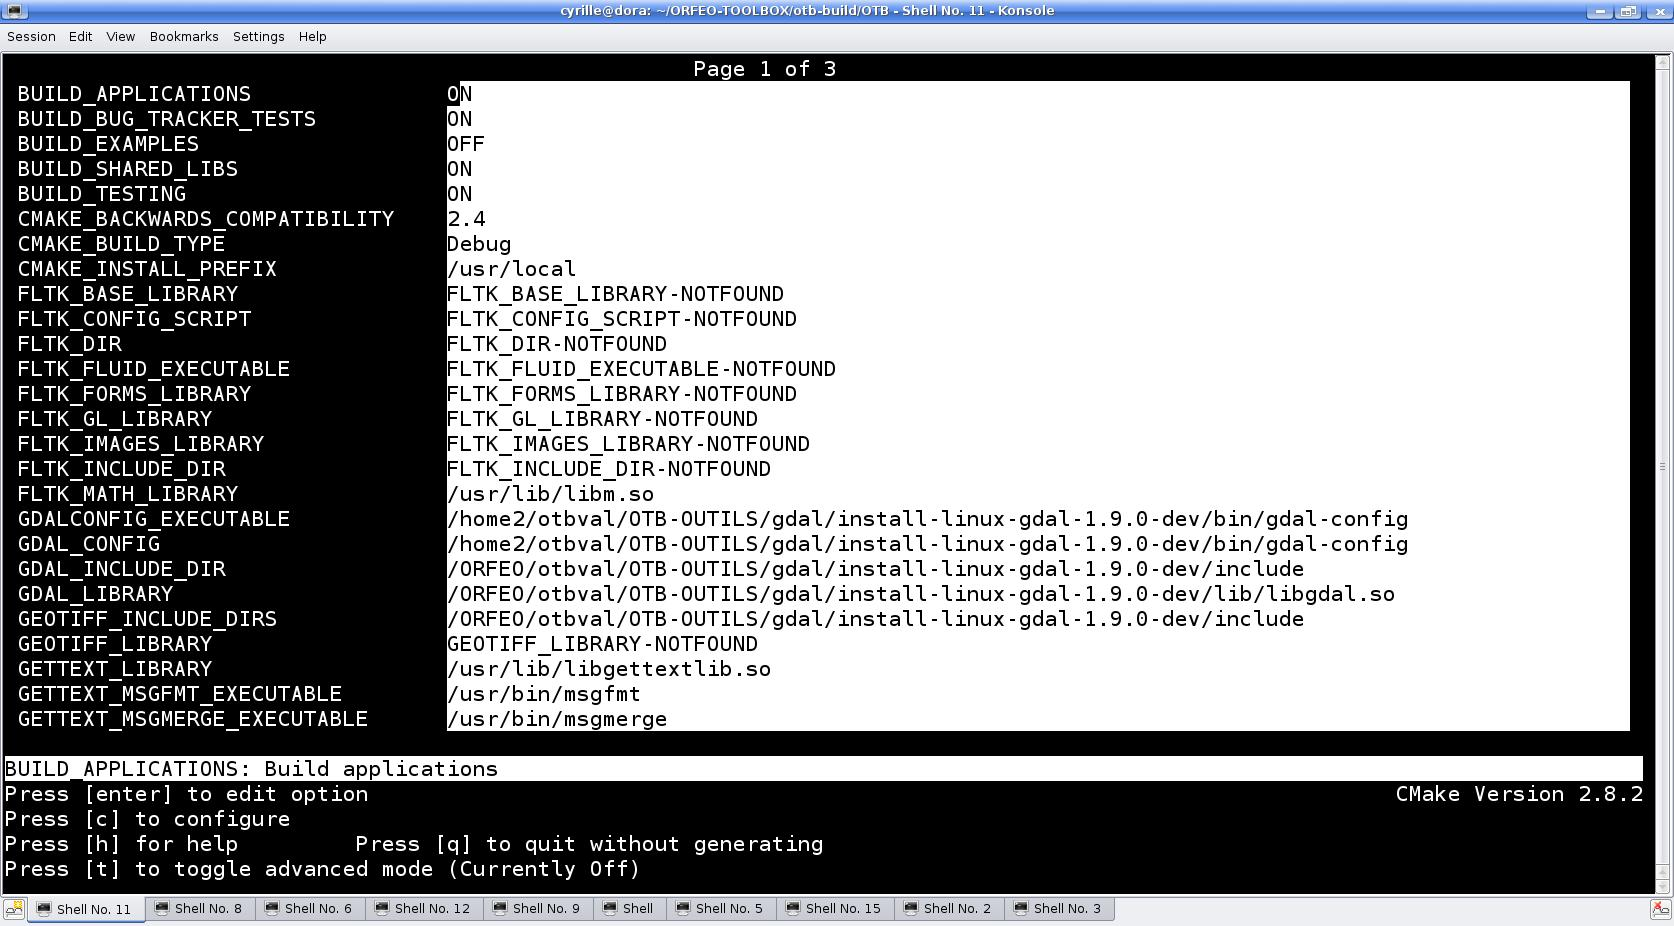
\includegraphics[width=0.8\textwidth]{ccmakeScreenShot.eps}
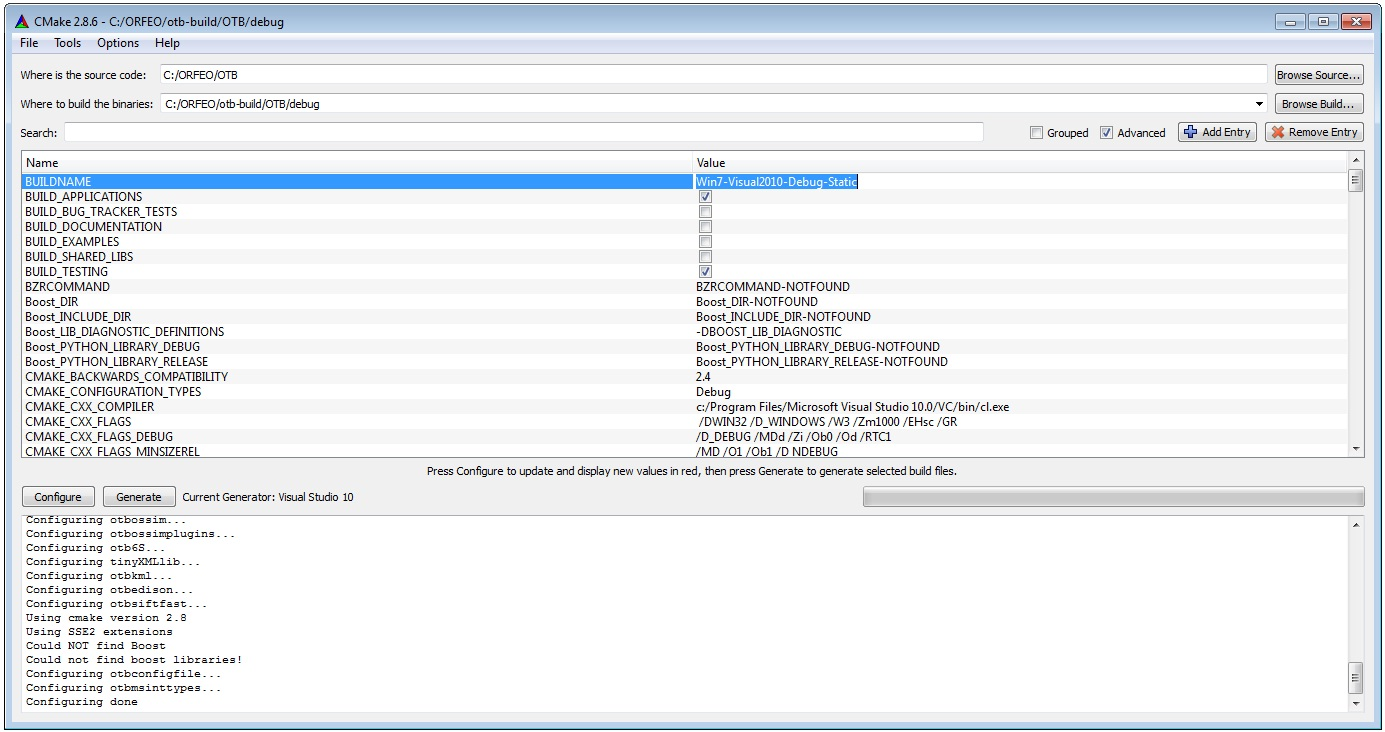
\includegraphics[width=0.8\textwidth]{CMakeSetupScreenShot.eps}
\itkcaption[Cmake user interface]{CMake interface. Top) \texttt{ccmake}, the UNIX
version based on \texttt{curses}. Bottom) \texttt{CMakeSetup}, the MS-Windows
version based on MFC.}
\label{fig:CMakeGUI}
\end{figure}

Figure \ref{fig:CMakeGUI} shows the CMake interface for UNIX and MS-Windows.
In order to speed up the build process you may want to disable the compilation
of the testing and examples. This is done with the variables
\code{BUILD\_TESTING=OFF} and \code{BUILD\_EXAMPLES=OFF}.  The examples
distributed with the toolbox are a helpful resource for learning how to use OTB
components but are not essential for the use of the toolbox itself. The testing
section includes a large number of small programs that exercise the
capabilities of OTB classes. Due to the large number of tests, enabling the
testing option will considerably increase the build time.  It is not
desirable to enable this option for a first build of the toolbox.

An additional resource is available in the \code{OTB-Applications} module,
which contains applications incorporating GUIs and different levels
of visualization.  However, building this module
should be postponed until you are familiar with the basic structure of the
toolbox and the building process.

Begin running CMake by using
ccmake on Unix, and CMakeSetup on
Windows. Remember to run ccmake from the binary directory on Unix. On
Windows, specify the source and binary directories in the GUI, then begin to
set the build variables in the GUI as necessary.  Most variables should have
default values that are sensible. Each time you change a set of variables in
CMake, it is necessary to proceed to another configuration step. In the
Windows version this is done by clicking on the ``Configure'' button. In the
UNIX version this is done in an interface using the
curses library, where you can configure by hitting the ``c'' key.

When no new options appear in CMake, you can proceed to generate Makefiles or
Visual Studio projects (or appropriate build file(s) depending on your
compiler). This is done in Windows by clicking on the ``Ok'' button.  In the
UNIX version this is done by hitting the ``g'' key. After the generation
process CMake will quit silently. To initiate the build process on UNIX,
simply type \code{make} in the binary directory. Under Windows, load the
workspace named \code{OTB.dsw} (if using MSDEV) or \code{OTB.sln} (if using
the .NET compiler) from the binary directory you specified in the CMake GUI.

The build process will typically take anywhere from 15 to 30 minutes depending
on the performance of your system. If you decide to enable testing as part of
the normal build process, about 600 small test programs will be compiled. This
will verify that the basic components of OTB have been correctly built on your
system.

\subsubsection{Building ITK}

The OTB installation procedure allows you to choose between building
the OTB with an external version of ITK already present in your
system. The choice is made by using the \code{OTB\_USE\_EXTERNAL\_ITK}
CMake variable.

\section{Getting Started With OTB }
\label{sec:GettingStartedWithOTB}

The simplest way to create a new project with OTB is to create a new directory
somewhere in your disk and create two files in it. The first one is a
\code{CMakeLists.txt} file that will be used by CMake to generate a Makefile
(if you are using UNIX) or a Visual Studio workspace (if you are using
MS-Windows).  The second file is an actual C++ program that will exercise
some of the large number of classes available in OTB. The details of these files
are described in the following section.

Once both files are in your directory you can run CMake in order to configure
your project. Under UNIX, you can cd to your newly created directory
and type ``\code{ccmake .}''. Note the ``.'' in the command line for indicating
that the \code{CMakeLists.txt} file is in the current directory. The
curses interface will require you to provide the directory where OTB
was built. This is the same path that you indicated for the
\code{OTB\_BINARY\_DIR} variable at the time of configuring OTB. Under
Windows you can run CMakeSetup and provide your newly created
directory as being both the source directory and the binary directory for
your new project (i.e., an in-source build). Then CMake will require you to
provide the path to the binary directory where OTB was built. The OTB binary
directory will contain a file named \code{OTBConfig.cmake} generated during the
configuration process at the time OTB was built.  From this file, CMake will
recover all the information required to configure your new OTB project.


\subsection{Hello World !}
\label{sec:HelloWorldOTB}

\index{Hello World}

Here is the content of the two files to write in your new project. These two
files can be found in the \code{OTB/Examples/Installation} directory. The
\code{CMakeLists.txt} file contains the following lines:

\small
\begin{verbatim}
PROJECT(HelloWorld)

FIND_PACKAGE(OTB REQUIRED)
INCLUDE(${OTB_USE_FILE})

ADD_EXECUTABLE(HelloWorld HelloWorld.cxx )
TARGET_LINK_LIBRARIES(HelloWorld OTBCommon OTBIO ITKCommon ITKIO)
\end{verbatim}

\normalsize

The first line defines the name of your project as it appears in Visual
Studio (it will have no effect under UNIX). The second line loads a CMake
file with a predefined strategy for finding OTB \footnote{Similar files are
provided in CMake for other commonly used libraries, all of them named
\code{Find*.cmake}}. If the strategy for finding OTB fails, CMake will prompt
you for the directory where OTB is installed in your system. In that case you
will write this information in the \code{OTB\_DIR} variable. The line \code{
INCLUDE(\$\{USE\_OTB\_FILE\})} loads the \code{UseOTB.cmake} file to set
all the configuration information from OTB.

%The next block of lines is needed in order for CMake to know whether you
%are using the OTB's internal version of ITK or an external one. In the
%second case, CMake will try to find ITK in your system. As for OTB, if
%it fails in finding ITK, it will ask you to manually set the ITK location.

The line \code{ADD\_EXECUTABLE}
defines as its first argument the name of the executable that will be produced
as result of this project. The remaining arguments of \code{ADD\_EXECUTABLE}
are the names of the source files to be compiled and linked.  Finally, the
\code{TARGET\_LINK\_LIBRARIES} line specifies which OTB libraries will be
linked against this project.


\input HelloWorld.tex

At this point you have successfully installed and compiled OTB, and created
your first simple program. If you have difficulties, please join the
otb-users mailing list (Section~\ref{sec:JoinMailList} on page
\pageref{sec:JoinMailList}) and post questions there.

\chapter{System Overview}
\label{chapter:SystemOverview}

The purpose of this chapter is to provide you with an overview of the
\emph{ORFEO Toolbox} system. We recommend that you read this chapter to
gain an appreciation for the breadth and area of application of
OTB. In this chapter, we will make reference either to \emph{OTB
  features} or \emph{ITK features} without distinction. Bear in mind
that OTB uses ITK as its core element, so all the fundamental elements
of OTB come from ITK. OTB extends the functionalities of ITK for the
remote sensing image processing comunity. We benefit from the Open
Source development approach chosen for ITK, which allows us to provide
an impressive set of functionalities with much lesser effort than it
would have been the case in a closed source universe!

\section{System Organization}
\label{sec:SystemOrganization}

The ORFEO Toolbox consists of several subsystems. A brief
description of these subsystems follows. Later sections in this chapter---and
in some cases additional chapters---cover these concepts in more detail. (Note:
in the previous chapter two other modules---\code{OTB-Documents} and
\code{OTB-Applications} were briefly described.)

\begin{description}
	\item[Essential System Concepts.] Like any software system, OTB is
        built around some core design concepts. OTB uses those of
        ITK. Some of the more important
        concepts include generic programming, smart pointers for memory
        management, object factories for adaptable object instantiation,
        event management using the command/observer design paradigm, and
        multithreading support.

	\item[Numerics] OTB, as ITK uses VXL's VNL numerics libraries. These are
        easy-to-use C++ wrappers around the Netlib Fortran numerical 
        analysis routines (\url{http://www.netlib.org}).

	\item[Data Representation and Access.]  Two principal classes
        are used to represent data: the \doxygen{otb}{Image} and
        \doxygen{itk}{Mesh} classes.  In addition, various types of
        iterators and containers are used in ITK to hold and traverse
        the data. Other important but less popular classes are also
        used to represent data such as histograms.

	\item[ITK's Data Processing Pipeline.]  The data representation
	classes (known as \emph{data objects}) are operated on by
	\emph{filters} that in turn may be organized into data flow
	\emph{pipelines}. These pipelines maintain state and therefore
	execute only when necessary.  They also support
	multi-threading, and are streaming capable (i.e., can operate
	on pieces of data to minimize the memory footprint).

        \item[IO Framework.] Associated with the data processing
        pipeline are \emph{sources}, filters that initiate the
        pipeline, and \emph{mappers}, filters that terminate the
        pipeline.  The standard examples of sources and mappers are
        \emph{readers} and \emph{writers} respectively.  Readers
        input data (typically from a file), and writers output data
        from the pipeline. \emph{Viewers} are another example of mappers.

	\item[Spatial Objects.] Geometric shapes are represented in
        OTB using the ITK spatial object hierarchy.  These classes are
        intended to support modeling of anatomical structures in
        ITK. OTB uses them in order to model cartographic elements. Using a
        common basic interface, the spatial objects are capable of
        representing regions of space in a variety of different
        ways. For example: mesh structures, image masks, and implicit
        equations may be used as the underlying representation scheme.
        Spatial objects are a natural data structure for communicating
        the results of segmentation methods and for introducing
        geometrical priors in both segmentation and registration
        methods.

	\item[ITK's Registration Framework.] A flexible framework for
        registration supports four different types of registration:
        image registration, multiresolution registration, PDE-based
        registration, and FEM (finite element method) registration.

	\item[FEM Framework.] ITK includes a subsystem for solving general
        FEM problems, in particular non-rigid registration. The FEM package
        includes mesh definition (nodes and elements), loads, and boundary
        conditions.

	\item[Level Set Framework.] The level set framework is a set of
        classes for creating filters to solve partial differential equations
        on images using an iterative, finite difference update scheme. The
        level set framework consists of finite difference solvers including a
        sparse level set solver, a generic level set segmentation filter, and
        several specific subclasses including threshold, Canny, and Laplacian
        based methods.

	\item[Wrapping.] ITK uses a unique, powerful system for
	producing interfaces (i.e., ``wrappers'') to interpreted
	languages such as Tcl and Python. The GCC\_XML tool is used to
	produce an XML description of arbitrarily complex C++ code;
	CSWIG is then used to transform the XML description into
	wrappers using the \href{http://www.swig.org/}{SWIG}
	package. OTB does not use this system at present.

	\item[Auxiliary / Utilities] Several auxiliary subsystems are 
        available to supplement other classes in the system. For example,
        calculators are classes that perform specialized operations in
        support of filters (e.g., MeanCalculator computes the mean of a
        sample). Other utilities include GDAL format file
        support, png, zlib, FLTK / Qt image viewers, and interfaces to the
        Visualization Toolkit (VTK) system.
        
\end{description}


\section{Essential System Concepts}
\label{sec:EssentialSystemConcepts}

This section describes some of the core concepts and implementation features
found in ITK and therefore also in OTB.

\subsection{Generic Programming}
\label{sec:GenericProgramming}

\index{generic programming}
\index{template}

Generic programming is a method of organizing libraries consisting of
generic---or reusable---software components \cite{Musser1996}. The idea is to
make software that is capable of ``plugging together'' in an efficient,
adaptable manner. The essential ideas of generic programming are
\emph{containers} to hold data, \emph{iterators} to access the data, and 
\emph{generic algorithms} that use containers and iterators to create 
efficient, fundamental algorithms such as sorting. Generic programming is
implemented in C++ with the \emph{template} programming mechanism and the 
use of the STL Standard Template Library \cite{Austern1999}.

C++ templating is a programming technique allowing users to write software in
terms of one or more unknown types \code{T}. To create executable code, the
user of the software must specify all types \code{T} (known as \emph{template
instantiation}) and successfully process the code with the compiler. The
\code{T} may be a native type such as
\code{float} or \code{int}, or \code{T} may be a user-defined type (e.g.,
\code{class}). At compile-time, the compiler makes sure that the templated 
types are compatible with the instantiated code and that the types are
supported by the necessary methods and operators.

ITK uses the techniques of generic programming in its implementation. The
advantage of this approach is that an almost unlimited variety of data types
are supported simply by defining the appropriate template types. For example,
in OTB it is possible to create images consisting of almost any type of
pixel. In addition, the type resolution is performed at compile-time, so the
compiler can optimize the code to deliver maximal performance. The
disadvantage of generic programming is that many compilers still do not
support these advanced concepts and cannot compile OTB. And even if they do,
they may produce completely undecipherable error messages due to even the
simplest syntax errors. If you are not familiar with templated code and
generic programming, we recommend the two books cited above.

\subsection{Include Files and Class Definitions}
\label{sec:IncludeFiles}

In ITK and OTB classes are defined by a maximum of two files: a header \code{.h} file
and an implementation file---\code{.cxx} if a non-templated class, and a
\code{.txx} if a templated class.
The header files contain class declarations
and formatted comments that are used by the Doxygen documentation
system to automatically produce HTML manual pages.

In addition to class headers, there are a few other important header files.
\begin{description}
        \item[\code{itkMacro.h}] is found in the
        \code{Utilities/ITK/Code/Common} directory
        and defines standard system-wide macros (such as \code{Set/Get},
        constants, and other parameters).

        \item[\code{itkNumericTraits.h}] is found in the \code{Utilities/ITK/Code/Common}
        directory and defines numeric characteristics for native types such
        as its maximum and minimum possible values.

        \item[\code{itkWin32Header.h}] is found in the \code{Utilities/ITK/Code/Common}
        and is used to define operating system parameters to control
        the compilation process.
\end{description}

\subsection{Object Factories}
\label{sec:ObjectFactories}

\index{object factory}
\index{factory}

Most classes in OTB are instantiated through an \emph{object factory}
mechanism. That is, rather than using the standard C++ class constructor and
destructor, instances of an OTB class are created with the static class
\code{New()} method. In fact, the constructor and destructor are
\code{protected:} so it is generally not possible to construct an OTB
instance on the heap. (Note: this behavior pertains to classes that are
derived from \doxygen{itk}{LightObject}. In some cases the need for speed or
reduced memory footprint dictates that a class not be derived from
LightObject and in this case instances may be created on the heap. An
example of such a class is \doxygen{itk}{EventObject}.)

The object factory enables users to control run-time instantiation of classes
by registering one or more factories with \doxygen{itk}{ObjectFactoryBase}. These
registered factories support the method \code{CreateInstance(classname)}
which takes as input the name of a class to create. The factory can choose to
create the class based on a number of factors including the computer system
configuration and environment variables. For example, in a particular
application an OTB user may wish to deploy their own class implemented using
specialized image processing hardware (i.e., to realize a performance
gain). By using the object factory mechanism, it is possible at run-time to
replace the creation of a particular OTB filter with such a custom class. (Of
course, the class must provide the exact same API as the one it is
replacing.) To do this, the user compiles her class (using the same compiler,
build options, etc.) and inserts the object code into a shared library or
DLL. The library is then placed in a directory referred to by the
\code{OTB\_AUTOLOAD\_PATH} environment variable. On instantiation, the object
factory will locate the library, determine that it can create a class of a
particular name with the factory, and use the factory to create the
instance. (Note: if the \code{CreateInstance()} method cannot find a factory
that can create the named class, then the instantiation of the class falls
back to the usual constructor.)

In practice object factories are used mainly (and generally transparently) by
the OTB input/output (IO) classes. For most users the greatest impact is on
the use of the \code{New()} method to create a class. Generally the
\code{New()} method is declared and implemented via the macro
\code{itkNewMacro()} found in \code{Utilities/ITK/Common/itkMacro.h}.


\subsection{Smart Pointers and Memory Management}
\label{sec:SmartPointers}

\index{smart pointer}

By their nature object-oriented systems represent and operate on data through
a variety of object types, or classes. When a particular class is
instantiated to produce an instance of that class, memory allocation occurs
so that the instance can store data attribute values and method pointers
(i.e., the vtable). This object may then be referenced by other classes or
data structures during normal operation of the program. Typically during
program execution all references to the instance may disappear at which point
the instance must be deleted to recover memory resources. Knowing when to
delete an instance, however, is difficult. Deleting the instance too soon
results in program crashes; deleting it too late and memory leaks (or
excessive memory consumption) will occur. This process of allocating and
releasing memory is known as memory management.

In ITK, memory management is implemented through reference counting. This
compares to another popular approach---garbage collection---used
\index{garbage collection} by many
systems including Java. In reference counting, a count of the number of
references to each instance is kept. When the reference goes to zero, the
object destroys itself. In garbage collection, a background process sweeps
the system identifying instances no longer referenced in the system and
deletes them. The problem with garbage collection is that the actual point in
time at which memory is deleted is variable. This is unacceptable when an
object size may be gigantic (think of a large 3D volume gigabytes in
size). Reference counting deletes memory immediately (once all references to
an object disappear).

Reference counting is implemented through a \code{Register()}/\code{Delete()}
member function interface.  All instances of an OTB object have a
\code{Register()} method invoked on them by any other object that references
an them. The \code{Register()} method increments the instances' reference
count. When the reference to the instance disappears, a \code{Delete()}
method is invoked on the instance that decrements the reference count---this
is equivalent to an \code{UnRegister()} method. When the reference count
returns to zero, the instance is destroyed.

This protocol is greatly simplified by using a helper class called a
\doxygen{itk}{SmartPointer}. The smart pointer acts like a regular pointer
(e.g. supports operators \code{->} and \code{*}) but automagically performs a
\code{Register()} when referring to an instance, and an \code{UnRegister()}
when it no longer points to the instance.  Unlike most other instances in
OTB, SmartPointers can be allocated on the program stack, and are
automatically deleted when the scope that the SmartPointer was created
is closed. As a result, you should \emph{rarely if ever call Register() or
Delete()} in OTB. For example:

\small
\begin{verbatim}
  MyRegistrationFunction()
    { <----- Start of scope

    // here an interpolator is created and associated to the
    // SmartPointer "interp".
    InterpolatorType::Pointer interp = InterpolatorType::New();

    } <------ End of scope
\end{verbatim}
\normalsize

In this example, reference counted objects are created (with the \code{New()}
method) with a reference count of one. Assignment to the SmartPointer
\code{interp} does not change the reference count. At the end of scope,
\code{interp} is destroyed, the reference count of the actual interpolator
object (referred to by \code{interp}) is decremented, and if it reaches zero,
then the interpolator is also destroyed.

Note that in ITK SmartPointers are always used to refer to instances of
classes derived from \doxygen{itk}{LightObject}. Method invocations and function
calls often return ``real'' pointers to instances, but they are immediately
assigned to a SmartPointer. Raw pointers are used for non-LightObject classes when
the need for speed and/or memory demands a smaller, faster class.


\subsection{Error Handling and Exceptions}
\label{sec:ErrorHandling}

\index{exceptions}
\index{error handling}

In general, OTB uses exception handling to manage errors during program
execution. Exception handling is a standard part of the C++ language and
generally takes the form as illustrated below:
\small
\begin{verbatim}
  try
    {
    //...try executing some code here...
    }
  catch ( itk::ExceptionObject exp )
    {
    //...if an exception is thrown catch it here
    }
\end{verbatim}
\normalsize

where a particular class may throw an exceptions as demonstrated below (this
code snippet is taken from \doxygen{itk}{ByteSwapper}:
\small
\begin{verbatim}
  switch ( sizeof(T) )
    {
    //non-error cases go here followed by error case  
    default:  
      ByteSwapperError e(__FILE__, __LINE__);
      e.SetLocation("SwapBE");
      e.SetDescription("Cannot swap number of bytes requested");
      throw e;
    }
\end{verbatim}
\normalsize

Note that \doxygen{itk}{ByteSwapperError} is a subclass of
\doxygen{itk}{ExceptionObject}. (In fact in OTB all exceptions should be derived
from \code{itk::ExceptionObject}.) In this example a special constructor and C++
preprocessor variables \code{\_\_FILE\_\_} and \code{\_\_LINE\_\_} are used to instantiate
the exception object and provide additional information to the user. You can
choose to catch a particular exception and hence a specific OTB error, or you
can trap \emph{any} OTB exception by catching ExceptionObject.


\subsection{Event Handling}
\label{sec:EventHandling}

\index{event handling}
\index{Command/Observer design pattern}
\index{itk::Command}
\index{ProgressEvent()}
\index{InvokeEvent()}

Event handling in OTB is implemented using the Subject/Observer design
pattern \cite{Gamma1995} (sometimes referred to as the Command/Observer
design pattern). In this approach, objects indicate that they are watching
for a particular event---invoked by a particular instance--by registering
with the instance that they are watching.  For example, filters in OTB
periodically invoke the \doxygen{itk}{ProgressEvent}. Objects that have registered
their interest in this event are notified when the event occurs. The
notification occurs via an invocation of a command (i.e., function callback,
method invocation, etc.) that is specified during the registration
process. (Note that events in OTB are subclasses of EventObject; look
in \code{itkEventObject.h} to determine which events are available.)

To recap via example: various objects in OTB will invoke specific events
as they execute (from ProcessObject):
\small
\begin{verbatim}
  this->InvokeEvent( ProgressEvent() );
\end{verbatim}
\normalsize

To watch for such an event, registration is required that associates a
command (e.g., callback function) with the event:
\code{Object::AddObserver()} method:
\small
\begin{verbatim}
  unsigned long progressTag = 
    filter->AddObserver(ProgressEvent(), itk::Command*);
\end{verbatim}
\normalsize

When the event occurs, all registered observers are notified via invocation
of the associated \code{Command::Execute()} method. Note that several
subclasses of Command are available supporting const and
non-const member functions as well as C-style functions. (Look in
\code{Common/Command.h} to find pre-defined subclasses of
Command. If nothing suitable is found, derivation is another
possibility.)

\subsection{Multi-Threading}
\label{sec:MultiThreading}

Multithreading is handled in OTB through ITK's high-level design
abstraction. This approach provides portable multithreading and hides the
complexity of differing thread implementations on the many systems supported
by OTB. For example, the class \doxygen{itk}{MultiThreader} provides support for
multithreaded execution using \code{sproc()} on an SGI, or
\code{pthread\_create} on any platform supporting POSIX threads. 

Multithreading is typically employed by an algorithm during its execution
phase. MultiThreader can be used to execute a single method on
multiple threads, or to specify a method per thread. For example, in the 
class \doxygen{itk}{ImageSource} (a superclass for most image processing filters)
the \code{GenerateData()} method uses the following methods:

\small
\begin{verbatim}
  multiThreader->SetNumberOfThreads(int);
  multiThreader->SetSingleMethod(ThreadFunctionType, void* data);
  multiThreader->SingleMethodExecute();
\end{verbatim}
\normalsize

In this example each thread invokes the same method. The multithreaded filter
takes care to divide the image into different regions that do not overlap for
write operations.

The general philosophy in ITK regarding thread safety is that accessing
different instances of a class (and its methods) is a thread-safe operation.
Invoking methods on the same instance in different threads is to be avoided.


\section{Numerics}
\label{sec:Numerics}

\index{VNL}
\index{numerics}

OTB; as ITK, uses the VNL numerics library to provide resources for numerical
programming combining the ease of use of packages like Mathematica and Matlab
with the speed of C and the elegance of C++. It provides a C++ interface to
the high-quality Fortran routines made available in the public domain by
numerical analysis researchers. ITK extends the functionality of VNL
by including interface classes between VNL and ITK proper.

The VNL numerics library includes classes for
\begin{description}
        \item[Matrices and vectors.] Standard matrix and vector support
        and operations on these types.

        \item[Specialized matrix and vector classes.] Several special matrix
        and vector class with special numerical properties are
        available. Class \code{vnl\_diagonal\_matrix} provides a fast and
        convenient diagonal matrix, while fixed size matrices and vectors
        allow "fast-as-C" computations (see \code{vnl\_matrix\_fixed<T,n,m>} 
        and example subclasses \code{vnl\_double\_3x3} and 
        \code{vnl\_double\_3}).

        \item[Matrix decompositions.] Classes \code{vnl\_svd<T>}, 
        \code{vnl\_symmetric\_eigensystem<T>}, and 
        \code{vnl\_generalized\_eigensystem}. 

        \item[Real polynomials.] Class \code{vnl\_real\_polynomial} stores 
        the coefficients of a real polynomial, and provides methods of 
        evaluation of the polynomial at any x, while class 
        \code{vnl\_rpoly\_roots} provides a root finder. 

        \item[Optimization.] Classes \code{vnl\_levenberg\_marquardt},
        \code{vnl\_amoeba}, \code{vnl\_conjugate\_gradient}, 
        \code{vnl\_lbfgs} allow optimization of user-supplied
        functions either with or without user-supplied derivatives.

        \item[Standardized functions and constants.] Class \code{vnl\_math}
        defines constants (pi, e, eps...) and simple functions (sqr, abs,
        rnd...). Class \code{numeric\_limits} is from the ISO standard
        document, and provides a way to access basic limits of a
        type. For example \code{numeric\_limits<short>::max()} returns the maximum
        value of a short.
\end{description}

Most VNL routines are implemented as wrappers around the high-quality Fortran
routines that have been developed by the numerical analysis community over
the last forty years and placed in the public domain. The central repository
for these programs is the "netlib" server \url{http://www.netlib.org/}. The
National Institute of Standards and Technology (NIST) provides an excellent
search interface to this repository in its \emph{Guide to Available Mathematical
Software (GAMS)} at \url{http://gams.nist.gov}, both as a decision tree and a
text search.

ITK also provides additional numerics functionality. A suite of optimizers, that
use VNL under the hood and integrate with the registration framework
are available. A large collection of statistics functions---not available from
VNL---are also provided in the \code{Insight/Numerics/Statistics}
directory. In addition, a complete finite element (FEM) package is available,
primarily to support the deformable registration in ITK.


\section{Data Representation}
\label{sec:DataRepresentationAndAccess}
%	mesh, image, iterators, various containers

\index{data object} 

There are two principle types of data represented in OTB: images and
meshes. This functionality is implemented in the classes 
Image and Mesh, both of which are subclasses of
\doxygen{itk}{DataObject}. In OTB, data objects are classes that are meant to
be passed around the system and may participate in data flow pipelines (see
Section~\ref{sec:DataProcessingPipeline} on
page~\pageref{sec:DataProcessingPipeline} for more information).


\index{otb::Image}

\doxygen{otb}{Image} represents an \emph{n}-dimensional, regular sampling of
data. The sampling direction is parallel to each of the coordinate axes, and
the origin of the sampling, inter-pixel spacing, and the number of samples in
each direction (i.e., image dimension) can be specified. The sample, or
pixel, type in OTB is arbitrary---a template parameter \code{TPixel}
specifies the type upon template instantiation. (The dimensionality of the
image must also be specified when the image class is instantiated.) The key
is that the pixel type must support certain operations (for example, addition
or difference) if the code is to compile in all cases (for example, to be
processed by a particular filter that uses these operations). In practice the
OTB user will use a C++ simple type (e.g., \code{int}, \code{float}) or a pre-defined pixel
type and will rarely create a new type of pixel class.

One of the important ITK concepts regarding images is that rectangular,
continuous pieces of the image are known as \emph{regions}. Regions are used
to specify which part of an image to process, for example in multithreading,
or which part to hold in memory. In ITK there are three common types of
regions:
\begin{enumerate}
\item \code{LargestPossibleRegion}---the image in its entirety.
\item \code{BufferedRegion}---the portion of the image retained in memory.
\item \code{RequestedRegion}---the portion of the region requested by a 
filter or other class when operating on the image.
\end{enumerate}

The \doxygen{otb}{Image} class extends the functionalities of the
\doxygen{itk}{Image} in order to take into account particular remote
sensing features as geographical projections, etc.

\index{itk::Mesh} 

The Mesh class represents an \emph{n}-dimensional, unstructured grid. The
topology of the mesh is represented by a set of \emph{cells} defined by a 
type and
connectivity list; the connectivity list in turn refers to points.  The
geometry of the mesh is defined by the \emph{n}-dimensional points in
combination with associated cell interpolation functions. \code{Mesh} is
designed as an adaptive representational structure that changes depending on
the operations performed on it. At a minimum, points and cells are required
in order to represent a mesh; but it is possible to add additional topological
information.  For example, links from the points to the cells that use each
point can be added; this provides implicit neighborhood information assuming
the implied topology is the desired one. It is also possible to
specify boundary cells explicitly, to indicate different connectivity
from the implied neighborhood relationships, or to store information
on the boundaries of cells. 

The mesh is defined in terms of three template parameters: 1) a pixel type
associated with the points, cells, and cell boundaries; 2) the dimension of
the points (which in turn limits the maximum dimension of the cells); and 3)
a ``mesh traits'' template parameter that specifies the types of the
containers and identifiers used to access the points, cells, and/or
boundaries. By using the mesh traits carefully, it is possible to create
meshes better suited for editing, or those better suited for ``read-only''
operations, allowing a trade-off between representation flexibility, memory,
and speed.

Mesh is a subclass of \doxygen{itk}{PointSet}. The PointSet
class can be used to represent point clouds or randomly distributed
landmarks, etc. The PointSet class has no associated topology.


\section{Data Processing Pipeline}
\label{sec:DataProcessingPipeline}

\index{data processing pipeline}

\index{process object} 
\index{source}
\index{reader} 
\index{filter} 
\index{mapper} 

While data objects (e.g., images and meshes) are used to represent data,
\emph{process objects} are classes that operate on data objects and may
produce new data objects. Process objects are classed as
\emph{sources}, \emph{filter objects}, or \emph{mappers}.  Sources (such as
readers) produce data, filter objects take in data and process it to produce
new data, and mappers accept data for output either to a file or
some other system.  Sometimes the term \emph{filter} is used broadly
to refer to all three types.

\index{streaming}

The data processing pipeline ties together data objects (e.g., images and
meshes) and process objects. The pipeline supports an automatic updating
mechanism that causes a filter to execute if and only if its input 
or its internal state changes. Further, the data pipeline supports
\emph{streaming}, the ability to automatically break data into smaller
pieces, process the pieces one by one, and reassemble the processed data into
a final result.

Typically data objects and process objects are connected together using the
\code{SetInput()} and \code{GetOutput()} methods as follows:

\small
\begin{verbatim}
  typedef otb::Image<float,2> FloatImage2DType;

  itk::RandomImageSource<FloatImage2DType>::Pointer random;
  random = itk::RandomImageSource<FloatImage2DType>::New();
  random->SetMin(0.0);
  random->SetMax(1.0);

  itk::ShrinkImageFilter<FloatImage2DType,FloatImage2DType>::Pointer shrink;
  shrink = itk::ShrinkImageFilter<FloatImage2DType,FloatImage2DType>::New();
  shrink->SetInput(random->GetOutput());
  shrink->SetShrinkFactors(2);

  otb::ImageFileWriter::Pointer<FloatImage2DType> writer;
  writer = otb::ImageFileWriter::Pointer<FloatImage2DType>::New();
  writer->SetInput (shrink->GetOutput());
  writer->SetFileName( ``test.raw'' );
  writer->Update();
\end{verbatim}
\normalsize 

In this example the source object \doxygen{itk}{RandomImageSource} is connected
to the \doxygen{itk}{ShrinkImageFilter}, and the shrink filter is connected to
the mapper \doxygen{otb}{ImageFileWriter}. When the \code{Update()} method is
invoked on the writer, the data processing pipeline causes each of these
filters in order, culminating in writing the final data to a file on disk.

%\section{Registration Framework}
%\label{sec:RegistrationFramework}
%
%blah blah
%
%\section{FEM Framework}
%\label{sec:FEMFramework}
%
%blah blah
%
\section{Spatial Objects}
\label{sec:SpatialObjectsOverview}
\index{spatial object}
%
The ITK spatial object framework supports the philosophy that the task of
image segmentation and registration is actually the task of object
processing. The image is but one medium for representing objects of interest,
and much processing and data analysis can and should occur at the object
level and not based on the medium used to represent the object.

ITK spatial objects provide a common interface for accessing the physical
location and geometric properties of and the relationship between objects in
a scene that is independent of the form used to represent those objects. That
is, the internal representation maintained by a spatial object may be a list
of points internal to an object, the surface mesh of the object, a continuous
or parametric representation of the object's internal points or surfaces, and
so forth.

The capabilities provided by the spatial objects framework supports their use
in object segmentation, registration, surface/volume rendering, and other
display and analysis functions. The spatial object framework extends the
concept of a ``scene graph'' \index{scene graph} that is common to computer rendering packages so
as to support these new functions. With the spatial objects framework you
can:
\begin{enumerate}

        \item Specify a spatial object's parent and children objects.  In
        this way, a city may contain roads and those roads can be
        organized in a tree structure.

        \item Query if a physical point is inside an object or
        (optionally) any of its children.

        \item Request the value and derivatives, at a physical point,
        of an associated intensity function, as specified
        by an object or (optionally) its children.

        \item Specify the coordinate transformation that maps a parent
        object's coordinate system into a child object's coordinate system.

        \item Compute the bounding box of a spatial object and (optionally)
        its children.

        \item Query the resolution at which the object was originally
        computed.  For example, you can query the resolution (i.e., pixel
        spacing) of the image used to generate a particular instance of a
        \doxygen{itk}{LineSpatialObject}.
\end{enumerate}

Currently implemented types of spatial objects include: Blob, Ellipse,
Group, Image, Line, Surface, and Tube.  The \doxygen{itk}{Scene}
object is used to hold a list of spatial objects that may in turn have
children.  Each spatial object can be assigned a color property.  Each
spatial object type has its own capabilities. For example,
\doxygen{itk}{TubeSpatialObject}s indicate to what point on their parent
tube they connect.

There are a limited number of spatial objects and their methods in ITK, but
their number is growing and their potential is huge. Using the nominal
spatial object capabilities, methods such as mutual
information registration, can be applied to objects regardless of their
internal representation. By having a common API, the same method can be used
to register a parametric representation of a building with an image or
to register two different segmentations of a particular object in
object-based change detection.

%blah blah
%
%\section{Level Set Framework}
%\label{sec:LevelSetFramework}
%
%blah blah
%
%% \section{Wrapping}
%% \label{sec:Wrapping}

%% \index{wrapping}
%% \index{Tcl}
%% \index{Python}

%% While the core of OTB is implemented in C++, Tcl and Python bindings can be
%% automatically generated and OTB programs can be created using these
%% programming languages. This capability is under active development and is for
%% the advanced user only. However, this brief description will give you an idea
%% of what is possible and where to look if you are interested in this facility.

%% The wrapping process in OTB is quite complex due to the use of generic
%% programming (i.e., extensive use of C++ templates). Systems like VTK that use
%% their own wrapping facility are non-templated and customized to the coding
%% methodology found in the system. Even systems like SWIG that are designed
%% for general wrapper generation have difficulty with OTB code because general
%% C++ is difficult to parse. As a result, the OTB wrapper generator uses a
%% combination of tools to produce language bindings.
%% \begin{enumerate}
%%   \item gccxml is a modified version of the GNU compiler gcc that
%%     produces an XML description of an input C++ program.
%%   \item  CABLE processes XML information from gccxml and produces
%%     additional input to the next tool (i.e., CSWIG indicating what is
%%     to be wrapped).
%%   \item CSWIG is a modified version of SWIG that has SWIG's usual
%%     parser replaced with an XML parser (XML produced from CABLE and
%%     gccxml.) CSWIG produces the appropriate language bindings
%%     (either Tcl or Python). (Note: since SWIG is capable of producing
%%     language bindings for eleven different interpreted languages including
%%     Java, and Perl, it is expected that support for some of these languages
%%     will be added in the future.)
%% \end{enumerate}

%% To learn more about the wrapping process, please read the file found in
%% \code{Wrapping/CSwig/README}. Also note that there are some simple test
%% scripts found in \code{Wrapping/CSwig/Tests}. Additional tests and examples
%% are found in the {Testing/Code/*/} directories.

%% The result of the wrapping process is a set of shared libraries/dll's that
%% can be used by the interpreted languages. There is almost a direct
%% translation from C++, with the differences being the particular syntactical
%% requirements of each language. For example, in the directory
%% \code{Testing/Code/Algorithms}, the test
%% \code{itkCurvatureFlowTestTcl2.tcl} has a code fragment that appears as
%% follows: 
%% \small
%% \begin{verbatim}
%%   set reader [itkImageFileReaderF2_New]
%%     $reader SetFileName "${OTB_TEST_INPUT}/cthead1.png"

%%   set cf [itkCurvatureFlowImageFilterF2F2_New]
%%     $cf SetInput [$reader GetOutput]
%%     $cf SetTimeStep 0.25
%%     $cf SetNumberOfIterations 10
%% \end{verbatim}
%% \normalsize
%% The same code in C++ would appear as follows:

%% \small
%% \begin{verbatim}
%%   otb::ImageFileReader<ImageType>::Pointer reader = 
%%               otb::ImageFileReader<ImageType>::New();
%%   reader->SetFileName("cthead1.png");

%%   itk::CurvatureFlowImageFilter<ImageType,ImageType>::Pointer cf =
%%       itk::CurvatureFlowImageFilter<ImageType,ImageType>::New();
%%     cf->SetInput(reader->GetOutput());
%%     cf->SetTimeStep(0.25);
%%     cf->SetNumberOfIterations(10);
%% \end{verbatim}
%% \normalsize

%% This example demonstrates an important difference between C++ and a wrapped
%% language such as Tcl.  Templated classes must be instantiated prior to
%% wrapping. That is, the template parameters must be specified as part of the
%% wrapping process. In the example above, the
%% \code{CurvatureFlowImageFilterF2F2} indicates that this filter has been
%% instantiated using an input and output image type of two-dimensional float
%% values (e.g., \code{F2}). Typically just a few common types are selected for
%% the wrapping process to avoid an explosion of types and hence, library
%% size. To add a new type requires rerunning the wrapping process to produce
%% new libraries.

%% The advantage of interpreted languages is that they do not require the
%% lengthy compile/link cycle of a compiled language like C++. Moreover, they
%% typically come with a suite of packages that provide useful
%% functionality. For example, the Tk package (i.e., Tcl/Tk and Python/Tk)
%% provides tools for creating sophisticated user interfaces. In the future it
%% is likely that more applications and tests will be implemented in the various
%% interpreted languages supported by OTB.


%
%blah blah
%
%\section{Auxiliary \& Utilities}
%\label{sec:Auxiliary}
%\label{sec:Utilities}
%
%calculators and classes supporting the data processing pipeline;
%utilities such as GUI interface tools



\part{User's guide}

\chapter{Data Representation}
\label{sec:DataRepresentation}


This chapter introduces the basic classes responsible
for representing data in OTB. The most common classes are the
\doxygen{otb::Image}, the \doxygen{itk::Mesh} and the \doxygen{itk::PointSet}.

\section{Image}
\label{sec:ImageSection}

The \doxygen{otb::Image} class follows the spirit of
\href{http://www.boost.org/more/generic_programming.html}{Generic
Programming}, where types are separated from the algorithmic behavior
of the class.  OTB supports images with any pixel type and any spatial
dimension.

\subsection{Creating an Image}\label{sec:CreatingAnImageSection}

\textbf{FIXME : update with otb::Image}
\input{Image1.tex}

In practice it is rare to allocate and initialize an image directly.
Images are typically read from a source, such a file or data acquisition
hardware. The following example illustrates how an image can be read from
a file.




\subsection{Reading an Image from a File}
\label{sec:ReadingImageFromFile}

\input{Image2.tex}





\subsection{Accessing Pixel Data}
\label{sec:AccessingImagePixelData}

\input{Image3.tex}




\subsection{Defining Origin and Spacing}
\label{sec:DefiningImageOriginAndSpacing}

\input{Image4.tex}

\subsection{Defining Other Image Attributes}
\label{sec:DefiningOtherImageAttributes}
%% Geographic projections, etc?

\subsection{RGB Images}

The term RGB (Red, Green, Blue) stands for a color representation commonly used
in digital imaging. RGB is a representation of the human physiological
capability to analyze visual light using three spectral-selective
sensors~\cite{Malacara2002,Wyszecki2000}. The human retina possess different
types of light sensitive cells. Three of them, known as \emph{cones}, are
sensitive to color~\cite{Gray2003} and their regions of sensitivity loosely
match regions of the spectrum that will be perceived as red, green and blue
respectively. The \emph{rods} on the other hand provide no color discrimination
and favor high resolution and high sensitivity\footnote{The human eye is
capable of perceiving a single isolated photon.}.  A fifth type of receptors,
the \emph{ganglion cells}, also known as circadian\footnote{The term
\emph{Circadian} refers to the cycle of day and night, that is, events that are
repeated with 24 hours intervals.} receptors are sensitive to the lighting
conditions that differentiate day from night.  These receptors evolved as a
mechanism for synchronizing the physiology with the time of the day. Cellular
controls for circadian rythms are present in every cell of an organism and are
known to be exquisitively precise~\cite{Lodish2000}.

The RGB space has been constructed as a representation of a physiological
response to light by the three types of \emph{cones} in the human eye. RGB is
not a Vector space. For example, negative numbers are not appropriate in a
color space because they will be the equivalent of ``negative stimulation'' on
the human eye.  In the context of colorimetry, negative color values are used
as an artificial construct for color comparison in the sense that

\begin{equation}
\label{eqn:ColorSubtraction}
         ColorA = ColorB - ColorC
\end{equation}

just as a way of saying that we can produce $ColorB$ by combining $ColorA$ and
$ColorC$.  However, we must be aware that (at least in emitted light) it is not
possible to \emph{substract light}. So when we mention
Equation~\ref{eqn:ColorSubtraction} we actually mean

\begin{equation}
\label{eqn:ColorAddition}
         ColorB = ColorA + ColorC
\end{equation}

On the other hand, when dealing with printed color and with paint, as opposed
to emitted light like in computer screens, the physical behavior of color
allows for subtraction. This is because strictly speaking the objects that we
see as red are those that absorb all light frequencies except those in the red
section of the spectrum~\cite{Wyszecki2000}.

The concept of addition and subtraction of colors has to be carefully
interpreted. In fact, RGB has a different definition regarding whether we are
talking about the channels associated to the three color sensors of the human
eye, or to the three phosphors found in most computer monitors or to the color
inks that are used for printing reproduction.  Color spaces are usually non
linear and do not even from a Group. For example, not all visible colors can be
represented in RGB space~\cite{Wyszecki2000}.

ITK introduces the \doxygen{itk::RGBPixel} type as a support for representing the
values of an RGB color space. As such, the RGBPixel class embodies a different
concept from the one of an \doxygen{itk::Vector} in space. For this reason, the
RGBPixel lack many of the operators that may be naively expected from it. In
particular, there are no defined operations for subtraction or addition.

When you anticipate to perform the operation of ``Mean'' on a RGB type you are
assuming that in the color space provides the action of finding a color in the
middle of two colors, can be found by using a linear operation between their
numerical representation. This is unfortunately not the case in  color spaces
due to the fact that they are based on a human physiological
response~\cite{Malacara2002}.

If you decide to interpret RGB images as simply three independent channels then
you should rather use the \doxygen{itk::Vector} type as pixel type. In this way, you
will have access to the set of operations that are defined in Vector spaces.
The current implementation of the RGBPixel in ITK presumes that RGB color
images are intended to be used in applications where a formal interpretation of
color is desired, therefore only the operations that are valid in a color space
are available in the RGBPixel class.

The following example illustrates how RGB images can be represented in OTB.

\label{sec:DefiningRGBImages}
\input{RGBImage.tex}


\subsection{Vector Images}
\label{sec:DefiningVectorImages}

\input{VectorImage.tex}


\subsection{Importing Image Data from a Buffer}
\label{sec:ImportingImageDataFromABuffer}
\input{Image5.tex}



\section{PointSet}
\label{PointSetSection}

\subsection{Creating a PointSet}
\label{sec:CreatingAPointSet}

\input{PointSet1.tex}



\subsection{Getting Access to Points}
\label{sec:GettingAccessToPointsInThePointSet}

\input{PointSet2.tex}



\subsection{Getting Access to Data in Points}
\label{sec:GettingAccessToDataInThePointSet}

\input{PointSet3.tex}



%\subsection{RGB as Pixel Type}
%\label{sec:PointSetWithRGBAsPixelType}

%\input{RGBPointSet.tex}




\subsection{Vectors as Pixel Type}
\label{sec:PointSetWithVectorsAsPixelType}

\input{PointSetWithVectors.tex}



%\subsection{Normals as Pixel Type}
%\label{sec:PointSetWithCovariantVectorsAsPixelType}

%\input{PointSetWithCovariantVectors.tex}




\section{Mesh}\label{MeshSection}

\subsection{Creating a Mesh}
\label{sec:CreatingAMesh}

\input{Mesh1.tex}


\subsection{Inserting Cells}
\label{sec:InsertingCellsInMesh}

\input{Mesh2.tex}


\subsection{Managing Data in Cells}
\label{sec:ManagingCellDataInMesh}

\input{Mesh3.tex}


More details about the use of \doxygen{itk::Mesh} can be found in the
ITK Software Guide.

%\subsection{Customizing the Mesh}
%\label{sec:CustomizingTheMesh}

%\input{MeshTraits.tex}


%\subsection{Topology and the K-Complex}
%\label{sec:MeshKComplex}

%\input{MeshKComplex.tex}


%\subsection{Representing a PolyLine}
%\label{sec:MeshPolyLine}

%\input{MeshPolyLine.tex}


%\subsection{Simplifying Mesh Creation}
%\label{sec:AutomaticMesh}

%\input{AutomaticMesh.tex}


%\subsection{Iterating Through Cells}
%\label{sec:MeshCellsIteration}

%\input{MeshCellsIteration.tex}


%\subsection{Visiting Cells}
%\label{sec:MeshCellVisitor}

%\input{MeshCellVisitor.tex}


%\subsection{More on Visiting Cells}
%\label{sec:MeshCellVisitorMultipleType}

%\input{MeshCellVisitor2.tex}




\section{Path}\label{PathSection}

\subsection{Creating a PolyLineParametricPath}
\label{sec:CreatingAPolyLineParametricPath}

\input{PolyLineParametricPath1.tex}

%\section{Containers}\label{ContainersSection}
%\label{sec:TreeContainer}
%\input{TreeContainer.tex}




\chapter{Reading and Writing Images}
\label{sec:IO}

This chapter describes the toolkit architecture supporting reading and
writing of images to files. OTB does not enforce any particular file
format, instead, it provides a structure inherited from ITK,
supporting a variety of formats that can be easily extended by the
user as new formats become available.

We begin the chapter with some simple examples of file I/O.

\section{Basic Example}
\label{sec:ImagReadWrite}
\input{ImageReadWrite.tex}

To better understand the IO architecture, please refer to Figures 
\ref{fig:ImageIOCollaborationDiagram}, 
\ref{fig:ImageIOFactoriesUseCases}, and
\ref{fig:ImageIOFactoriesClassDiagram}. 

\begin{figure}
\center
\includegraphics[width=\textwidth]{ImageIOCollaborationDiagram.eps}
\itkcaption[Collaboration diagram of the ImageIO classes]{Collaboration diagram
of the ImageIO classes.} \label{fig:ImageIOCollaborationDiagram}
\end{figure}

\begin{figure}
\center
\includegraphics[width=\textwidth]{ImageIOFactoriesUseCases.eps}
\itkcaption[Use cases of ImageIO factories] {Use cases of ImageIO factories.}
\label{fig:ImageIOFactoriesUseCases}
\end{figure}

\begin{figure}
\center
\includegraphics[width=\textwidth]{ImageIOFactoriesClassDiagram.eps}
\itkcaption[Class diagram of ImageIO factories] {Class diagram of the ImageIO
factories.}
\label{fig:ImageIOFactoriesClassDiagram}
\end{figure}


The following section describes the internals of the IO architecture provided
in the toolbox.

\section{Pluggable Factories}
\label{sec:ImageIOPluggableFactories}

The principle behind the input/output mechanism used in ITK and
therefore OTB is known as
\emph{pluggable-factories} \cite{Gamma1995}. This concept is illustrated in
the UML diagram in Figure~\ref{fig:ImageIOCollaborationDiagram}. From the
user's point of view the objects responsible for reading and writing files
are the \doxygen{otb}{ImageFileReader} and \doxygen{otb}{ImageFileWriter}
classes. These two classes, however, are not aware of the details involved in
reading or writing particular file formats like PNG or GeoTIFF.  What they do
is to dispatch the user's requests to a set of specific classes that are
aware of the details of image file formats. These classes are the
\doxygen{itk}{ImageIO} classes. The ITK delegation mechanism enables users to
extend the number of supported file formats by just adding new classes to the
ImageIO hierarchy.

Each instance of ImageFileReader and ImageFileWriter has
a pointer to an ImageIO object. If this pointer is empty, it will
be impossible to read or write an image and the image file reader/writer must
determine which ImageIO class to use to perform IO operations.
This is done basically by passing the filename to a centralized class, the
\doxygen{itk}{ImageIOFactory} and asking it to identify any subclass of
ImageIO capable of reading or writing the user-specified file. This
is illustrated by the use cases on the right side of
Figure~\ref{fig:ImageIOFactoriesUseCases}. The ImageIOFactory acts here as a
dispatcher that help to locate the actual IO factory classes corresponding to
each file format.

Each class derived from ImageIO must provide an associated factory
class capable of producing an instance of the ImageIO class. For
example, for PNG files, there is a \doxygen{itk}{PNGImageIO} object that knows how
to read this image files and there is a \doxygen{itk}{PNGImageIOFactory} class
capable of constructing a PNGImageIO object and returning a pointer
to it.  Each time a new file format is added (i.e., a new ImageIO
subclass is created), a factory must be implemented as a derived class of the
ObjectFactoryBase class as illustrated in
Figure~\ref{fig:ImageIOFactoriesClassDiagram}.

For example, in order to read PNG files, a PNGImageIOFactory is
created and registered with the central ImageIOFactory
singleton\footnote{\emph{Singleton} means that there is only one instance of
this class in a particular application} class as illustrated in the left side
of Figure~\ref{fig:ImageIOFactoriesUseCases}. When the ImageFileReader asks
the ImageIOFactory for an ImageIO capable of reading the
file identified with \emph{filename} the ImageIOFactory will iterate over the
list of registered factories and will ask each one of them is they know how
to read the file. The factory that responds affirmatively will be used to
create the specific ImageIO instance that will be returned to the
ImageFileReader and used to perform the read operations.

With respect to the ITK formats, OTB adds most of the remote sensing
image formats. In order to do so, the Geospatial Data Abstraction Library, GDAL
      \url{http://www.gdal.org/}, is encapsultated in a ImageIO
      factory. GDAL is a translator library for raster
      geospatial data formats that is released under an X/MIT style
      Open Source license. As a library, it presents a single abstract
      data model to the calling application for all supported formats,
      which include CEOS, GeoTIFF, ENVI, and much more. See
      \url{http://www.gdal.org/formats_list.html} for
      the full format list.

      Since GDAL is itself a multi-format library, the GDAL IO
factory is able to choose the appropriate ressource for reading and
writing images. 

In most cases the mechanism is transparent to the user who only interacts
with the ImageFileReader and ImageFileWriter. It is
possible, however, to explicitly select the type of ImageIO object
to use.  Please see the ITK Software for more details about this.

%\section{Using ImageIO Classes Explicitly}
%\label{sec:ImageReadExportVTK}
%\input{ImageReadExportVTK.tex}

\section{IO Streaming}
\index{Streaming}
\label{sec:IOStreaming}
\subsection{Implicit Streaming}
\label{sec:ImplicitIOStreaming}
\input{StreamingImageReadWrite}

\subsection{Explicit Streaming}
\label{sec:ExplicitIOStreaming}
\input{ExplicitStreamingExample}


\section{Reading and Writing RGB Images}
\index{Image!RGB}
\label{sec:RGBImagReadWrite}
\input{RGBImageReadWrite.tex}

\section{Reading, Casting and Writing Images}
\label{sec:ImagReadCastWrite}
\input{ImageReadCastWrite.tex}

\section{Extracting Regions}
\label{sec:ImagReadRegionOfInterestWrite}
\input{ImageReadRegionOfInterestWrite.tex}

%\section{Extracting Slices}
%\label{sec:ImagReadExtractWrite}
%\input{ImageReadExtractWrite.tex}


\section{Reading and Writing Vector Images}
\index{Image!Multispectral}
\label{sec:VectorImagReadWrite}

Images whose pixel type is a Vector, a CovariantVector, an Array, or a Complex
are quite common in image processing. One of the uses of these tye of
images is the processing of SLC SAR images, which are complex.


%\subsection{The Minimal Example}
%\label{VectorImageReadWrite}
%\input{VectorImageReadWrite.tex}

%\subsection{Producing and Writing Covariant Images}
%\label{CovariantVectorImageWrite}
%\input{CovariantVectorImageWrite.tex}

%\subsection{Reading Covariant Images}
%\label{CovariantVectorImageRead}
%Let's now take the image that we just created and read it into another program.
%\input{CovariantVectorImageRead.tex}


\subsection{Reading and Writing Complex Images}
\label{sec:ComplexImagReadWrite}
\input{ComplexImageReadWrite.tex}

\section{Reading and Writing Multiband Images}
\label{sec:MultibandImagReadWrite}
\input{MultibandImageReadWrite.tex}

\subsection{Extracting ROIs}
\label{sec:ExtractROI}
\input{ExtractROI.tex}


%\section{Extracting Components from Vector Images}
%\label{sec:VectorImageExtractComponent}
%\input{CovariantVectorImageExtractComponent.tex}

\section{Reading Image Series}
\label{sec:Reading Image Series}
\input{ImageSeriesIOExample}

%% \section{Reading and Writing Image Series}

%% It is still quite common to store 3D medical images in sets of files each one
%% containing a single slice of a volume dataset. Those 2D files can be read as
%% individual 2D images, or can be grouped together in order to reconstruct a 3D
%% dataset. The same practice can be extended to higher dimensions, for example,
%% for managing 4D datasets by using sets of files each one containing a 3D image.
%% This practice is common in the domain of cardiac imaging, perfusion, functional
%% MRI and PET. This section illustrates the functionalities available in ITK for
%% dealing with reading and writing series of images.

%% \index{Series!Reading}
%% \index{Series!Writing}
%% \index{Image Series!Reading}
%% \index{Image Series!Writing}

%% \subsection{Reading Image Series}
%% \label{sec:ReadingImageSeries}
%% \input{ImageSeriesReadWrite.tex}

%% \subsection{Writing Image Series}
%% \label{sec:WritingImageSeries}
%% %\input{ImageReadImageSeriesWrite.tex}

%% \subsection{Reading and Writing Series of RGB Images}
%% \label{sec:ReadingWritingRGBImageSeries}
%% %\input{RGBImageSeriesReadWrite.tex}


\section{Reading and Writing Vector Data}
\index{vector data}
\label{sec:ReadingVectorData}
In Remote Sensing the use of vector data is common. Vector data is
used to represent cartographic objects, segmentation results, etc:  
basically, everything which can be seen as point, line or polygons. OTB
provides functionnalities for accessing this kind of data.

\subsection{Lidar data Files}
\index{vector data!lidar}
\label{sec:ReadLidar}
\input{LidarReaderExample.tex}
\input{LidarToImageExample.tex}

\subsection{Reading DXF Files}
\index{vector data!dxf}
\label{sec:ReadDXF}
\input{DXFReaderExample.tex}

\subsection{Reading and Writing Vector Data Files}
\index{vector data!shapefile}
\label{sec:ReadVectorData}
\input{VectorDataIOExample.tex}


\section{Reading DEM Files}
\index{Digital elevation model}
\label{sec:ReadDEM}
\input{DEMToImageGenerator.tex}

\chapter{Basic Filtering}


This chapter introduces the most commonly used filters found in OTB.
Most of these filters are intended to process images. They will accept one or
more images as input and will produce one or more images as output. OTB is
based ITK's data pipeline architecture in which the output of one filter is
passed as input to another filter. (See Section
\ref{sec:DataProcessingPipeline} on page \pageref{sec:DataProcessingPipeline}
for more information.)


\section{Thresholding}
\ifitkFullVersion
\label{sec:ThresholdingFiltering}
\fi

The thresholding operation is used to change or identify pixel values based
on specifying one or more values (called the \emph{threshold} value). The
following sections describe how to perform thresholding operations using
OTB.

\subsection{Binary Thresholding}
\label{sec:BinaryThresholdingImageFilter}

\ifitkFullVersion
\input{BinaryThresholdImageFilter.tex}
\fi

\subsection{General Thresholding}
\label{sec:ThresholdingImageFilter}

\ifitkFullVersion
\input{ThresholdImageFilter.tex}
\fi

\subsection{Threshold to Point Set}
\label{sec:ThresholdImageToPointSetFilter}

\ifitkFullVersion
\input{ThresholdToPointSetExample.tex}
\fi


%% \section{Casting and Intensity Mapping}
%% \label{sec:CastingImageFilters}

%% The filters discussed in this section perform pixel-wise intensity mappings.
%% Casting is used to convert one pixel type to another, while intensity mappings
%% also take into account the different intensity ranges of the pixel types.

%% \subsection{Linear Mappings}
%% \label{sec:IntensityLinearMapping}

%% \ifitkFullVersion
%% %\input{CastingImageFilters.tex}
%% \fi

%% \subsection{Non Linear Mappings}
%% \label{sec:IntensityNonLinearMapping}

%% The following filter can be seen as a variant of the casting filters. Its main
%% difference is the use of a smooth and continuous transition function of
%% non-linear form.

%% \ifitkFullVersion
%% %\input{SigmoidImageFilter.tex}
%% \fi

\section{Gradients}
\label{sec:GradientFiltering}

Computation of gradients is a fairly common operation in image processing. The
term ``gradient'' may refer in some contexts to the gradient vectors and in
others to the magnitude of the gradient vectors. ITK filters attempt to
reduce this ambiguity by including the \emph{magnitude} term when
appropriate. ITK provides filters for computing both the image of gradient
vectors and the image of magnitudes.

\subsection{Gradient Magnitude}
\label{sec:GradientMagnitudeImageFilter}

\ifitkFullVersion
\input{GradientMagnitudeImageFilter.tex}
\fi

\subsection{Gradient Magnitude With Smoothing}
\label{sec:GradientMagnitudeRecursiveGaussianImageFilter}

\ifitkFullVersion
\input{GradientMagnitudeRecursiveGaussianImageFilter.tex}
\fi


\subsection{Derivative Without Smoothing}
\label{sec:DerivativeImageFilter}

\ifitkFullVersion
\input{DerivativeImageFilter.tex}
\fi


\section{Second Order Derivatives}
\label{sec:SecondOrderDerivatives}


%% \subsection{Second Order Recursive Gaussian}
%% \label{sec:SecondDerivativeRecursiveGaussian}

%% \ifitkFullVersion
%% \input{SecondDerivativeRecursiveGaussianImageFilter.tex}
%% \fi


\subsection{Laplacian Filters}
\label{sec:LaplacianFilters}

%\subsubsection{Laplacian Filter Finite Difference}
\subsubsection{Laplacian Filter Recursive Gaussian}
\ifitkFullVersion
\input{LaplacianRecursiveGaussianImageFilter1.tex}
\input{LaplacianRecursiveGaussianImageFilter2.tex}
\fi




\section{Edge Detection}

\subsection{Canny Edge Detection}
\ifitkFullVersion
\input{CannyEdgeDetectionImageFilter.tex}
\fi

\subsection{Ratio of Means Detector }
\input{TouziEdgeDetectorExample}




\section{Neighborhood Filters}
\label{sec:NeighborhoodFilters}

The concept of locality is frequently encountered in image processing in the
form of filters that compute every output pixel using information from a small
region in the neighborhood of the input pixel.  The classical form of
these filters are the $3 \times 3$ filters in 2D images. Convolution masks
based on these neighborhoods can perform diverse tasks ranging from noise
reduction, to differential operations, to mathematical morphology.

The Insight toolkit implements an elegant approach to neighborhood-based image
filtering.  The input image is processed using a special iterator called the
\doxygen{itk}{NeighborhoodIterator}. This iterator is capable of moving over all the
pixels in an image and, for each position, it can address the pixels in a local
neighborhood. Operators are defined that apply an algorithmic operation in the
neighborhood of the input pixel to produce a value for the output pixel.  The
following section describes some of the more commonly used filters that take
advantage of this construction. (See Chapter
\ref{sec:ImageIteratorsChapter} on page
\pageref{sec:ImageIteratorsChapter} for more information about iterators.)

\subsection{Mean Filter}
\label{sec:MeanFilter}

\ifitkFullVersion
% Please do NOT edit this file.
% It has been automatically generated
% by a perl script from the original cxx sources
% in the Insight/Examples directory

% Any changes should be made in the file
% /ORFEO/thomas/ORFEO-TOOLBOX/OTB/Examples/StartExamples/MeanImageFilter.cxx


Le code source se trouve dans le fichier\\
\texttt{Examples/StartExamples/MeanImageFilter.cxx}.


  BLA BLA...

  \begin{center}
  \begin{picture}(200,46)
  \put(   5.0,  0.0 ){\framebox(30.0,15.0){25}} 
  \put(  35.0,  0.0 ){\framebox(30.0,15.0){30}} 
  \put(  65.0,  0.0 ){\framebox(30.0,15.0){32}} 
  \put(   5.0, 15.0 ){\framebox(30.0,15.0){27}} 
  \put(  35.0, 15.0 ){\framebox(30.0,15.0){25}} 
  \put(  65.0, 15.0 ){\framebox(30.0,15.0){29}} 
  \put(   5.0, 30.0 ){\framebox(30.0,15.0){28}} 
  \put(  35.0, 30.0 ){\framebox(30.0,15.0){26}} 
  \put(  65.0, 30.0 ){\framebox(30.0,15.0){50}} 
  \put( 100.0, 22.0 ){\vector(1,0){20.0}}
  \put( 125.0, 15.0 ){\framebox(34.0,15.0){30.22}} 
  \put( 160.0, 22.0 ){\vector(1,0){20.0}}
  \put( 185.0, 15.0 ){\framebox(30.0,15.0){30}} 
  \end{picture}
  \end{center}

  Suite BLA BLA...

  \index{itk::MeanImageFilter}


  The header file corresponding to this filter should be included first.

  \index{itk::MeanImageFilter!header}

\small
\begin{verbatim}
#include "itkMeanImageFilter.h"
\end{verbatim}
\normalsize
  
    Then the pixel types for input and output image must be defined and, with
    them, the image types can be instantiated.
  
\small
\begin{verbatim}
  typedef   unsigned char  InputPixelType;
  typedef   unsigned char  OutputPixelType;

  typedef itk::Image< InputPixelType,  2 >   InputImageType;
  typedef itk::Image< OutputPixelType, 2 >   OutputImageType;
\end{verbatim}
\normalsize
  
    Using the image types it is now possible to instantiate the filter type
    and create the filter object. 
  
    \index{itk::MeanImageFilter!instantiation}
    \index{itk::MeanImageFilter!New()}
    \index{itk::MeanImageFilter!Pointer}
   
\small
\begin{verbatim}
  typedef itk::MeanImageFilter<
               InputImageType, OutputImageType >  FilterType;

  FilterType::Pointer filter = FilterType::New();
\end{verbatim}
\normalsize
  
    The size of the neighborhood is defined along every dimension by
    passing a \code{SizeType} object with the corresponding values. The
    value on each dimension is used as the semi-size of a rectangular
    box. For example, in $2D$ a size of \(1,2\) will result in a $3 \times
    5$ neighborhood.
  
    \index{itk::MeanImageFilter!Radius}
    \index{itk::MeanImageFilter!Neighborhood}
  
\small
\begin{verbatim}
  InputImageType::SizeType indexRadius;
  
  indexRadius[0] = atoi(argv[3]); // radius along x
  indexRadius[1] = atoi(argv[4]); // radius along y

  filter->SetRadius( indexRadius );
\end{verbatim}
\normalsize
  
    The input to the filter can be taken from any other filter, for example
    a reader. The output can be passed down the pipeline to other filters,
    for example, a writer. An update call on any downstream filter will
    trigger the execution of the mean filter.
  
    \index{itk::MeanImageFilter!SetInput()}
    \index{itk::MeanImageFilter!GetOutput()}
  
\small
\begin{verbatim}
  filter->SetInput( reader->GetOutput() );
  writer->SetInput( filter->GetOutput() );
  writer->Update();
\end{verbatim}
\normalsize
   
   \begin{figure}
   \center
   \includegraphics[width=0.44\textwidth]{Circle.eps}
   
\includegraphics[width=0.44\textwidth]{CircleMeanOutput.eps}
   \itkcaption[Effect of the MedianImageFilter]{Effect of the MeanImageFilter on point.}
   \label{fig:CircleMeanOutput}
   \end{figure}
  
    Figure \ref{fig:CircleMeanOutput} illustrates the effect of this
    filter on an image of a point avec voisinage de \(10,10\) correspondant a un filtre de taille $ 21 \times 21 $.
  

\fi

\subsection{Median Filter}
\label{sec:MedianFilter}

\ifitkFullVersion
\input{MedianImageFilter.tex}
\fi


\subsection{Mathematical Morphology}
\label{sec:MathematicalMorphology}

Mathematical morphology has proved to be a powerful resource for image
processing and analysis \cite{Serra1982}. ITK implements mathematical
morphology filters using NeighborhoodIterators and
\doxygen{itk}{NeighborhoodOperator}s.  The toolkit contains two types of image
morphology algorithms, filters that operate on binary images and filters that
operate on grayscale images.

\subsubsection{Binary Filters}
\label{sec:MathematicalMorphologyBinaryFilters}

\ifitkFullVersion
\input{MathematicalMorphologyBinaryFilters.tex}
\fi


\subsubsection{Grayscale Filters}
\label{sec:MathematicalMorphologyGrayscaleFilters}

\ifitkFullVersion
\input{MathematicalMorphologyGrayscaleFilters.tex}
\fi


%% \subsection{Voting Filters}
%% \label{sec:VotingFilters}

%% Voting filters are quite a generic family of filters. In fact, both the Dilate
%% and Erode filters from Mathematical Morphology are very particular cases of the
%% broader family of voting filters. In a voting filter, the outcome of a pixel is
%% decided by counting the number of pixels in its neighborhood and applying a
%% rule to the result of that counting.For example, the typical implementation of
%% Erosion in terms of a voting filter will be to say that a foreground pixel will
%% become background if the numbers of background neighbors is greater or equal
%% than 1. In this context, you could imagine variations of Erosion in which the
%% count could be changed to require at least 3 foreground.

%% \subsubsection{Binary Median Filter}

%% One of the particular cases of Voting filters is the BinaryMedianImageFilter.
%% This filter is equivalent to applying a Median filter over a binary image. The
%% fact of having a binary image as input makes possible to optimize the execution
%% of the filter since there is no real need for sorting the pixels according to
%% their frequency in the neighborhood.

%% \ifitkFullVersion
%% %\input{BinaryMedianImageFilter.tex}
%% \fi

%% The typical effect of median filtration on a noisy digital image is a dramatic reduction in impulse noise spikes. The filter also tends to preserve brightness differences across signal steps, resulting in reduced blurring of regional boundaries. The filter also tends to preserve the positions of boundaries in an image.

%% Figure \ref{fig:BinaryMedianImageFilterOutputMultipleIterations} below shows the effect of running the median filter with a 3x3 classical window size 
%% 1, 10 and 50 times. There is a tradeoff in noise reduction and the sharpness of the image when the window size is increased\begin{figure}
%%   \center
%%   \includegraphics[width=0.44\textwidth]{BinaryMedianImageFilterOutput1.eps}
%%   \includegraphics[width=0.44\textwidth]{BinaryMedianImageFilterOutput10.eps}
%%   \includegraphics[width=0.44\textwidth]{BinaryMedianImageFilterOutput50.eps}
%%   \itkcaption[Effect of many iterations on the BinaryMedian filter.]{Effect of 1, 10 and 50 iterations of the
%%   BinaryMedianImageFilter using a 3x3 window.}
%%   \label{fig:BinaryMedianImageFilterOutputMultipleIterations}
%% \end{figure}.


%% \subsubsection{Hole Filling Filter}

%% Another variation of Voting filters is the Hole Filling filter. This filter
%% converts background pixels into foreground only when the number of foreground
%% pixels is a majority of the neighbors. By selecting the size of the majority,
%% this filter can be tuned to fill-in holes of different size. To be more
%% precise, the effect of the filter is actually related to the curvature of the
%% edge in which the pixel is located.

%% \ifitkFullVersion
%% %\input{VotingBinaryHoleFillingImageFilter.tex}
%% \fi


%% \subsubsection{Iterative Hole Filling Filter}

%% The Hole Filling filter can be used in an iterative way, by applying it
%% repeatedly until no pixel changes. In this context, the filter can be seen as a
%% binary variation of a Level Set filter.

%% \ifitkFullVersion
%% %\input{VotingBinaryIterativeHoleFillingImageFilter.tex}
%% \fi

\section{Smoothing Filters}
\label{sec:SmoothingFilters}

Real image data has a level of uncertainty that is manifested in the
variability of measures assigned to pixels. This uncertainty is usually
interpreted as noise and considered an undesirable component of the image
data. This section describes several methods that can be applied to reduce
noise on images.

\subsection{Blurring}
\label{sec:BlurringFilters}

Blurring is the traditional approach for removing noise from images. It is
usually implemented in the form of a convolution with a kernel. The effect of
blurring on the image spectrum is to attenuate high spatial
frequencies.  Different kernels attenuate frequencies in different ways. One
of the most commonly used kernels is the Gaussian. Two implementations of
Gaussian smoothing are available in the toolkit. The first one is based on a
traditional convolution while the other is based on the application of IIR
filters that approximate the convolution with a Gaussian
\cite{Deriche1990,Deriche1993}.

\subsubsection{Discrete Gaussian}
\label{sec:DiscreteGaussianImageFilter}

\ifitkFullVersion
\input{DiscreteGaussianImageFilter.tex}
\fi


%% \subsubsection{Binomial Blurring}
%% \label{sec:BinomialBlurImageFilter}

%% \ifitkFullVersion
%% %\input{BinomialBlurImageFilter.tex}
%% \fi

%% \subsubsection{Recursive Gaussian IIR}
%% \label{sec:RecursiveGaussianImageFilter}

%% \ifitkFullVersion
%% %\input{SmoothingRecursiveGaussianImageFilter.tex}
%% \fi


%% \subsection{Local Blurring}
%% \label{sec:BlurringFunctions}

%% In some cases it is desirable to compute smoothing in restricted regions of the
%% image, or to do it using different parameters that are computed locally.  The
%% following sections describe options for applying local smoothing in images.

%% \subsubsection{Gaussian Blur Image Function}
%% \label{sec:GaussianBlurImageFunction}

%% \ifitkFullVersion
%% %\input{GaussianBlurImageFunction.tex}
%% \fi

\subsection{Edge Preserving Smoothing}
\label{sec:EdgePreservingSmoothingFilters}

\subsubsection{Introduction to Anisotropic Diffusion}
\label{sec:IntroductionAnisotropicDiffusion}
\ifitkFullVersion
%
%
%  This file in inserted in the Filtering.tex file.
%
%

The drawback of image denoising (smoothing) is that it tends to blur away the
sharp boundaries in the image that help to distinguish between the
larger-scale anatomical structures that one is trying to characterize (which
also limits the size of the smoothing kernels in most applications).  Even in
cases where smoothing does not obliterate boundaries, it tends to distort the
fine structure of the image and thereby changes subtle aspects of the
anatomical shapes in question.

Perona and Malik \cite{Perona1990} introduced an alternative to
linear-filtering that they called \emph{anisotropic diffusion}.  Anisotropic
diffusion is closely related to the earlier work of Grossberg
\cite{Grossberg1984}, who used similar nonlinear diffusion processes to model
human vision.  The motivation for anisotropic diffusion (also called
\emph{nonuniform} or \emph{variable conductance} diffusion) is that a Gaussian
smoothed image is a single time slice of the solution to the heat equation, 
that has the original image as its initial conditions.  Thus, the solution to
\begin{equation} \frac{\partial g(x, y, t) }{\partial t} = \nabla \cdot \nabla
g(x, y, t), \end{equation} where $g(x, y, 0) = f(x, y)$ is the input image, is
$g(x, y, t) = G(\sqrt{2t}) \otimes f(x, y)$, where $G(\sigma)$ is a Gaussian
with standard deviation $\sigma$.  

Anisotropic diffusion includes a variable conductance term that, in turn,
depends on the differential structure of the image.  Thus, the variable
conductance can be formulated to limit the smoothing at ``edges'' in images, as
measured by high gradient magnitude, for example. \begin{equation} g_{t} = \nabla \cdot
c(\left| \nabla g \right|) \nabla g, \label{eq:aniso} \end{equation} where, for
notational convenience, we leave off the independent parameters of $g$ and use
the subscripts with respect to those parameters to indicate partial
derivatives.  The function $c(|\nabla g|)$ is a fuzzy cutoff that reduces the
conductance at areas of large $|\nabla g|$, and can be any one of a number of
functions.  The literature has shown \begin{equation} c(|\nabla g|) =
e^{-\frac{|\nabla g|^{2}}{2k^{2}}} \end{equation} to be quite effective.
Notice that conductance term introduces a free parameter $k$, the {\em
conductance parameter}, that controls the sensitivity of the process to edge
contrast.  Thus, anisotropic diffusion entails two free parameters: the
conductance parameter, $k$, and the time parameter, $t$, that is analogous to
$\sigma$, the effective width of the filter when using Gaussian kernels.

Equation \ref{eq:aniso} is a nonlinear partial differential equation that can
be solved on a discrete grid using finite forward differences.  Thus, the
smoothed image is obtained only by an iterative process, not a convolution or
non-stationary, linear filter.  Typically, the number of iterations required
for practical results are small, and large 2D images can be processed in
several tens of seconds using carefully written code running on modern, general
purpose, single-processor computers.  The technique applies readily and
effectively to 3D images, but requires more processing time.

In the early 1990's several research groups \cite{Gerig1991,Whitaker1993d}
demonstrated the effectiveness of anisotropic diffusion on medical images.  In
a series of papers on the subject
\cite{Whitaker1993,Whitaker1993b,Whitaker1993c,Whitaker1993d,Whitaker-thesis,Whitaker1994},
Whitaker described a detailed analytical and empirical analysis, introduced a
smoothing term in the conductance that made the process more robust, invented a
numerical scheme that virtually eliminated directional artifacts in the
original algorithm, and generalized anisotropic diffusion to vector-valued
images, an image processing technique that can be used on vector-valued medical
data (such as the color cryosection data of the Visible Human Project).

For a vector-valued input $\vec{F}:U \mapsto \Re^{m}$ the process takes the
form \begin{equation} \vec{F}_{t} = \nabla \cdot c({\cal D}\vec{F}) \vec{F},
\label{eq:vector_diff} \end{equation} where ${\cal D}\vec{F}$ is a {\em
dissimilarity} measure of $\vec{F}$, a generalization of the gradient magnitude
to vector-valued images, that can incorporate linear and nonlinear coordinate
transformations on the range of $\vec{F}$.  In this way, the smoothing of the
multiple images associated with vector-valued data is coupled through the
conductance term, that fuses the information in the different images.  Thus
vector-valued, nonlinear diffusion can combine low-level image features (e.g.
edges) across all ``channels'' of a vector-valued image in order to preserve or
enhance those features in all of image ``channels''.

Vector-valued anisotropic diffusion is useful for denoising data from devices
that produce multiple values such as MRI or color photography.  When performing
nonlinear diffusion on a color image, the color channels are diffused
separately, but linked through the conductance term. Vector-valued diffusion it
is also useful for processing registered data from different devices or for
denoising higher-order geometric or statistical features from scalar-valued
images \cite{Whitaker1994,Yoo1993}.

The output of anisotropic diffusion is an image or set of images that
demonstrates reduced noise and texture but preserves, and can also enhance,
edges.  Such images are useful for a variety of  processes including
statistical classification, visualization, and geometric feature extraction.
Previous work has shown \cite{Whitaker-thesis} that anisotropic diffusion, over
a wide range of conductance parameters, offers quantifiable advantages over
linear filtering for edge detection in medical images.

Since the effectiveness of nonlinear diffusion was first demonstrated, numerous
variations of this approach have surfaced in the literature \cite{Romeny1994}.
These include alternatives for constructing dissimilarity measures
\cite{Sapiro1996}, directional (i.e., tensor-valued) conductance terms
\cite{Weickert1996,Alvarez1994} and level set interpretations
\cite{Whitaker2001}.

\fi


\subsubsection{Gradient Anisotropic Diffusion}
\label{sec:GradientAnisotropicDiffusionImageFilter}

\ifitkFullVersion
\input{GradientAnisotropicDiffusionImageFilter.tex}
\fi



%% \subsubsection{Curvature Anisotropic Diffusion}
%% \label{sec:CurvatureAnisotropicDiffusionImageFilter}

%% \ifitkFullVersion
%% %\input{CurvatureAnisotropicDiffusionImageFilter.tex}
%% \fi

%% \subsubsection{Curvature Flow}
%% \label{sec:CurvatureFlowImageFilter}

%% \ifitkFullVersion
%% %\input{CurvatureFlowImageFilter.tex}
%% \fi

%% \subsubsection{MinMaxCurvature Flow}
%% \label{sec:MinMaxCurvatureFlowImageFilter}

%% \ifitkFullVersion
%% %\input{MinMaxCurvatureFlowImageFilter.tex}
%% \fi


%% \subsubsection{Bilateral Filter}
%% \label{sec:BilateralImageFilter}

%% \ifitkFullVersion
%% %\input{BilateralImageFilter.tex}
%% \fi




%% \subsection{Edge Preserving Smoothing in Vector Images}
%% \label{sec:VectorAnisotropicDiffusion}

%% Anisotropic diffusion can also be applied to images whose pixels are vectors.
%% In this case the diffusion is computed independently for each vector
%% component.  The following classes implement versions of anisotropic diffusion
%% on vector images.

%% \subsubsection{Vector Gradient Anisotropic Diffusion}
%% \label{sec:VectorGradientAnisotropicDiffusionImageFilter}

%% \ifitkFullVersion
%% %\input{VectorGradientAnisotropicDiffusionImageFilter.tex}
%% \fi

%% \subsubsection{Vector Curvature Anisotropic Diffusion}
%% \label{sec:VectorCurvatureAnisotropicDiffusionImageFilter}

%% \ifitkFullVersion
%% %\input{VectorCurvatureAnisotropicDiffusionImageFilter.tex}
%% \fi



%% \subsection{Edge Preserving Smoothing in Color Images}
%% \label{sec:ColorAnisotropicDiffusion}

%% \subsubsection{Gradient Anisotropic Diffusion}
%% \label{sec:ColorGradientAnisotropicDiffusion}

%% \ifitkFullVersion
%% %\input{RGBGradientAnisotropicDiffusionImageFilter.tex}
%% \fi

%% \subsubsection{Curvature Anisotropic Diffusion}
%% \label{sec:ColorCurvatureAnisotropicDiffusion}

%% \ifitkFullVersion
%% %\input{RGBCurvatureAnisotropicDiffusionImageFilter.tex}
%% \fi

\subsection{Edge Preserving Speckle Reduction Filters}
\label{sec:SpeckleFilters}
\ifitkFullVersion
\input{LeeImageFilter.tex}
\fi



\section{Distance Map}
\label{sec:DistanceMap}

\ifitkFullVersion
\input{DanielssonDistanceMapImageFilter.tex}
\fi

%% \ifitkFullVersion
%% %\input{SignedDanielssonDistanceMapImageFilter.tex}
%% \fi




%% \section{Geometric Transformations}
%% \label{sec:GeometricalTransformationFilters}

%% \subsection{Filters You Should be Afraid to Use}

%% \label{sec:ScaryImageFilters}
%% \subsection{Change Information Image Filter}

%% This one is the scariest and more dangerous filter in the entire toolkit. You
%% should not use this filter unless you are entirely certain that you know what
%% you are doing. In fact if you decide to use this filter, you should write your
%% code, then go for a long walk, get more coffee and ask yourself if you really
%% needed to use this filter. If the answer is yes, then you should discuss this
%% issue with someone you trust and get his/her opinion in writing.  In general,
%% if you need to use this filter, it means that you have a poor image provider
%% that is putting your career at risk along with the life of any potential
%% patient whose images you may end up processing.

%% \subsection{Flip Image Filter}

%% \ifitkFullVersion
%% %\input{FlipImageFilter.tex}
%% \fi

%% \subsection{Resample Image Filter}
%% \label{sec:ResampleImageFilter}

%% \subsubsection{Introduction}

%% \ifitkFullVersion
%% %\input{ResampleImageFilter.tex}
%% \fi

%% \subsubsection{Importance of Spacing and Origin}
%% \ifitkFullVersion
%% %\input{ResampleImageFilter2.tex}
%% \fi

%% \subsubsection{A Complete Example}
%% \ifitkFullVersion
%% %\input{ResampleImageFilter3.tex}
%% \fi

%% \subsubsection{Rotating an Image}
%% \ifitkFullVersion
%% %\input{ResampleImageFilter4.tex}
%% \fi

%% \subsubsection{Rotating and Scaling an Image}
%% \ifitkFullVersion
%% %\input{ResampleImageFilter5.tex}
%% \fi

%% \subsubsection{Resampling using a deformation field}
%% \ifitkFullVersion
%% %\input{WarpImageFilter1.tex}
%% \fi


%% \subsubsection{Subsampling and image in the same space}
%% \label{SubsampleVolume}

%% \ifitkFullVersion
%% %\input{SubsampleVolume.tex}
%% \fi



%% \subsubsection{Resampling an Anisotropic image to make it Isotropic}
%% \label{ResampleVolumesToBeIsotropic}

%% \ifitkFullVersion
%% %\input{ResampleVolumesToBeIsotropic.tex}
%% \fi



%% \section{Frequency Domain}
%% \label{sec:FrequencyDomain}


%% \subsection{Computing a Fast Fourier Transform (FFT)}
%% \label{FFTImageFilter}

%% \ifitkFullVersion
%% %\input{FFTImageFilter.tex}
%% \fi


%% \subsection{Filtering on the Frequency Domain}
%% \label{FFTImageFilterFourierDomainFiltering}

%% \ifitkFullVersion
%% %\input{FFTImageFilterFourierDomainFiltering.tex}
%% \fi



%% \section{Extracting Surfaces}
%% \label{sec:ExtractingSurfaces}

%% \subsection{Surface extraction}
%% \label{sec:SufaceExtraction}
%% \index{Surface Extraction}

%% \ifitkFullVersion
%% %\input{SurfaceExtraction.tex}
%% \fi






\chapter{Feature Extraction}

% \section{Introduction}

Under the term {\em Feature Extraction} we include several techniques
aiming to detect or extract informations of low level of abstraction
from images. These {\em features} can be objects : points, lines,
etc. They can also be measures : moments, textures, etc.

\section{Textures}
\subsection{Haralick Descriptors}
\input{TextureExample}

\subsection{PanTex}
\input{PanTexExample}

\section{Interest Points}
\subsection{Harris detector}
\input{HarrisExample}
\subsection{SIFT detector}
\label{sec:SIFTDetector}
\input{SIFTFastExample}
\subsection{SURF detector}
\input{SURFExample}

\section{Alignments}
\label{sec:Alignments}
\input{AlignmentsExample}
\section{Lines}
\label{sec:LineDetectors}

\subsection{Line Detection}
\label{sec:LineDetection}
\input{RatioLineDetectorExample}
\input{CorrelationLineDetectorExample}
\input{AssymmetricFusionOfLineDetectorExample}
\input{ParallelLineDetectionExample}


\subsection{Segment Extraction}
\label{sec:SegmentExtraction}
\subsubsection{Local Hough Transform}
\input{LocalHoughExample}
%\input{ExtractSegmentsByStepsExample}
%\input{ExtractSegmentsExample}
\subsubsection{Line Segment Detector}
\label{sec:LSD}
\input{LineSegmentDetectorExample}

\section{Density Features}
An interesting approach to feature extraction consists in computing
the density of previously detected features as simple edges or
interest points.
\subsection{Edge Density}
\input{EdgeDensityExample}
\subsection{SIFT Density}
\input{SIFTDensityExample}

\section{Geometric Moments}

\subsection{Complex Moments}
\label{sec:ComplexMoments}
The complex geometric moments are defined as:
\begin {equation}
c_{pq} = \int\limits_{-\infty}^{+\infty}\int\limits_{-\infty}^{+\infty}(x + iy)^p(x- iy)^qf(x,y)dxdy,
\label{2.2}
\end{equation}
where $x$ and $y$ are the coordinates of the image $f(x,y)$, $i$ is the
imaginary unit and
$p+q$ is the order of $c_{pq}$. The geometric moments are
particularly useful in the case of scale changes.

\subsubsection{Complex Moments for Images}
\input{ComplexMomentImageExample}
\subsubsection{Complex Moments for Paths}
\input{ComplexMomentPathExample}

\subsection{Hu Moments}
\label{sec:HuMoments}
Using the algebraic moment theory, H. Ming-Kuel obtained a family of 7
invariants with respect to planar transformations called Hu invariants,
\cite{hu}. Those invariants can be seen as nonlinear combinations of
the complex moments. Hu invariants have
been very much used in object recognition during the last 30 years,
since they are invariant to rotation, scaling and translation. \cite{flusserinv} gives their expressions :

\begin{equation}
\begin{array}{cccc}
\phi_1 = c_{11};& \phi_2 = c_{20}c_{02};& \phi_3 = c_{30}c_{03};& \phi_4 = c_{21}c_{12};\\
\phi_5 = Re(c_{30}c_{12}^3);& \phi_6 = Re(c_{21}c_{12}^2);& \phi_7 = Im(c_{30}c_{12}^3).&\\
\end{array}
\end{equation}


\cite{dudani} have used these invariants for the recognition of
aircraft silhouettes. Flusser and Suk have used them for image
registration, \cite{flusser_2}.

\subsubsection{Hu Moments for Images}
\input{HuMomentImageExample}
%\subsubsection{Hu Moments for Paths}
%\input{HuMomentPathExample}


\subsection{Flusser Moments}
\label{sec:FlusserMoments}
The Hu invariants have been modified and
improved by several authors. Flusser used these moments in order to
produce a new family of descriptors of order higher than 3,
\cite{flusserinv}. These descriptors are invariant to scale and
rotation. They have the following expressions:
\begin {equation}
\begin{array}{ccc}
\psi_1  = c_{11} = \phi_1; &  \psi_2  = c_{21}c_{12} = \phi_4; & \psi_3  = Re(c_{20}c_{12}^2) = \phi_6;\\
\psi_4  = Im(c_{20}c_{12}^2); & \psi_5  = Re(c_{30}c_{12}^3) = \phi_5;
& \psi_6  = Im(c_{30}c_{12}^3) = \phi_7.\\
\psi_7  = c_{22}; & \psi_8  = Re(c_{31}c_{12}^2); & \psi_9  = Im(c_{31}c_{12}~2);\\
\psi_{10} = Re(c_{40}c_{12}^4); & \psi_{11} = Im(c_{40}c_{12}^2). &\\

\end{array}
\end {equation}

\textbf{Examples}
\subsubsection{Flusser Moments for Images}
\input{FlusserMomentImageExample}
%\subsubsection{Flusser Moments for Paths}
%\input{FlusserMomentPathExample}

\section{Principal Component Analysis}
Principal Component Analysis is a linear projection technique which
can be used for dimensionality reduction.
\input{InnerProductPCAExample}

\section{Road extraction}
\label{sec:RoadExtraction}

Road extraction is a critical feature for an efficient use of high resolution satellite images. There are many applications of road extraction: update of GIS database, reference for image registration, help for identification algorithms and rapid mapping for example.  Road network can be used to register an optical image with a map or an optical image with a radar image for example. Road network extraction can help for other algorithms: isolated building detection, bridge detection. In these cases, a rough extraction can be sufficient. In the context of response to crisis, a fast mapping is necessary: within 6~hours, infrastructures for the designated area are required. Within this timeframe, a manual extraction is inconceivable and an automatic help is necessary.

\subsection{Road extraction filter}

\input{ExtractRoadExample}

\subsection{Step by step road extraction}

\input{ExtractRoadByStepsExample}


% \section{Seam carving}
% \label{sec:SeamCarving}
%
% \input{SeamCarvingExample}
%
% \input{SeamCarvingOtherExample}

\section{Cloud Detection}
\input{CloudDetectionExample}
\chapter{Image Segmentation}

\chapter{Change Detection}
\section{Introduction}
Change detection techniques try to detect and locate areas which have
changed between two or more observations of the same scene. These
changes can be of different types, with different origins and of
different temporal length. This allows to distinguish different kinds
of applications:
\begin{itemize}
\item \emph{land use monitoring}, which corresponds to the
  characterization of the evolution of the vegetation, or its seasonal
  changes;
\item \emph{natural resources management}, which corresponds mainly
  to the characterisation of the evolution of the urban areas, the
  evolution of the deforestation, etc.
\item \emph{damage mapping}, which corresponds to the location of
  damages caused by natural or industrial disasters.
\end{itemize}

From the point of view of the observed phenomena, one can distinguish
2 types of changes whose nature is rather different: the abrupt
changes and the progressive changes, which can eventually be
periodic. From the data point of view, one can have:

       \begin{itemize}
       \item Image pairs before and after the event. The applications
       are mainly the abrupt changes.

	 \item Multi-temporal image series on which 2 types on changes
	 may appear:
	 \begin{itemize}
	   \item The slow changes like for instance the erosion,
	   vegetation evolution, etc. The knowledge of the studied
	   phenomena and of their consequences on the geometrical
	   and radiometrical evolution at the different dates is a
	   very important information for this kind of analysis.

	     \item The abrupt changes may pose different kinds of
	     problems depending on whether the date of the change is
	     known in the image series or not. The detection of areas
	     affected by a change occurred at a known date may exploit
	     this a priori information in order to split the image
	     series into two sub-series (before an after) and use the
	     temporal redundancy in order to improve the detection
	     results. On the other hand, when the date of the change
	     is not known, the problem has a higher difficulty.

	 \end{itemize}
	 
       \end{itemize}

From this classification of the different types of problems, one can
infer 4 cases for which one can look for algorithms as a function of
the available data:
\begin{enumerate}
\item Abrupt changes in an image pair. This is no doubt the field for
  which more work has been done. One can find tools at the 3 classical
  levels of image processing: data level (differences, ratios, with
  or without pre-filtering, etc.), feature level (edges, targets,
  etc.), and interpretation level (post-classification comparison).

\item Abrupt changes within an image series and a known date. One can
  rely on bi-date techniques, either by fusing the images into 2 stacks
  (before and after), or by fusing the results obtained by different
  image couples (one after and one before the event). One can also use
  specific discontinuity detection techniques to be applied in the
  temporal axis.

\item Abrupt changes within an image series and an unknown date. This
  case can be seen either as a generalization of the preceding one (testing
  the N-1 positions for N dates) or as a particular case of the
  following one.

\item Progressive changes within an image series. One can work in two
  steps:
  \begin{enumerate}
    \item detect the change areas using stability criteria in the
    temporal areas;
    \item identify the changes using prior information about the type
    of changes of interest.
  \end{enumerate}
  
\end{enumerate}




\subsection{Surface-based approaches}\label{secChgtAbr}
In this section we discuss about the damage assessment techniques
which can be applied when only two images (before/after) are available.\\

As it has been shown in recent review works
\cite{Coppin03,Lu04,Radke05,Richards05}, a relatively high number of
methods exist, but most of them have been developed for optical and
infrared sensors. Only a few recent works on change detection with
radar images exist
\cite{Stabel02,Bruzzone02b,Onana_2003,Inglada03,Derrode03,Bazi05,Inglada07}.
However, the intrinsic limits of passive sensors, mainly related to
their dependence on meteorological and illumination conditions, impose
severe constraints for operational applications. The principal
difficulties related to change detection are of four types:

\begin{enumerate}
\item In the case of radar images, the speckle noise makes the image
  exploitation difficult.
\item The geometric configuration of the image acquisition can produce
  images which are difficult to compare.
\item Also, the temporal gap between the two acquisitions an thus the
  sensor aging and the inter-calibration are sources of variability
  which are difficult to deal with.
\item Finally, the normal evolution of the observed scenes must not be
  confused with the changes of interest.
\end{enumerate}

The problem of detecting abrupt changes between a pair of images is
the following: Let $I_{1},I_{2}$ be two images acquired at different
dates $t_{1},t_{2}$; we aim at producing a thematic map which shows
the areas where changes have taken place.

Three main categories of methods exist:

\begin{itemize}
\item{Strategy $1$: Post Classification Comparison}

The principle of this approach \cite{Deer_1998} is two obtain two
land-use maps independently for each date and comparing them. 



\item{Strategy $2$: Joint classification}

This method consists in producing the change map directly from a joint
classification of both images.

\item{Strategy $3$: Simple detectors}

The last approach consists in producing an image of change likelihood
(by differences, ratios or any other approach) and thresholding it in
order to produce the change map.

\end{itemize}


Because of its simplicity and its low computation overhead, the third
strategy is the one which has been chosen for the processing
presented here.



\section{Change Detection Framework}
\label{sec:ChangeDetectionFramework}
\input{ChangeDetectionFrameworkExample.tex}
\section{Simple Detectors}
\label{sec:SimpleDetectors}
\subsection{Mean Difference}
\label{sec:MeanDifference}

The simplest change detector is based on the pixel-wise differencing
of image values: 
\begin{equation}
I_{D}(i,j)=I_{2}(i,j)-I_{1}(i,j).
\end{equation}

In order to make the algorithm robust to noise, one actually uses
local means instead of pixel values.

\input{DiffChDet}

\subsection{Ratio Of Means}
\label{sec:RatioOfMeans}

This detector is similar to the previous one except that it uses a
ratio instead of the difference:
\begin{equation}
\displaystyle I_{R}(i,j) = \frac{\displaystyle I_{2}(i,j)}{\displaystyle I_{1}(i,j)}.
\end{equation}

The use of the ratio makes this detector robust to multiplicative
noise which is a good model for the speckle phenomenon which is
present in radar images.

In order to have a bounded and normalized detector the following
expression is actually used:


\begin{equation}
\displaystyle I_{R}(i,j) = 1 - min \left(\frac{\displaystyle I_{2}(i,j)}{\displaystyle I_{1}(i,j)},\frac{\displaystyle I_{1}(i,j)}{\displaystyle I_{2}(i,j)}\right).
\end{equation}


\input{RatioChDet}


\section{Statistical Detectors}
\label{sec:StatisticalDetectors}

\subsection{Distance between local distributions}
\label{sec:KullbackLeiblerDistance}

This detector is similar to the ratio of means detector (seen in the 
previous section page~\pageref{sec:RatioOfMeans}). Nevertheless, 
instead of the comparison of means, the comparison is performed to
the complete distribution of the two Random Variables (RVs)~\cite{Inglada03}.

The detector is based on the Kullback-Leibler distance between probability 
density functions (pdfs). In the neighborhood of each pixel of the pair 
of images $I_1$ and $I_2$ to be compared, the distance between local pdfs 
$f_1$ and $f_2$ of RVs $X_1$ and $X_2$ is evaluated by:
\begin{align}
  {\cal K}(X_1,X_2) &= K(X_1|X_2) + K(X_2|X_1) \\
  \text{with} \qquad
  K(X_j | X_i) &= \int_{\mathbbm{R}} 
      \log \frac{f_{X_i}(x)}{f_{X_j}(x)} f_{X_i}(x) dx,\qquad i,j=1,2.
\end{align}
In order to reduce the computational time, the local pdfs $f_1$ and $f_2$ 
are not estimated through histogram computations but rather by a cumulant
expansion, namely the Edgeworth expansion, with is based on the 
cumulants of the RVs:
\begin{equation}\label{eqEdgeworthExpansion}
f_X(x) = \left( 1 + \frac{\kappa_{X;3}}{6} H_3(x) 
					+ \frac{\kappa_{X;4}}{24} H_4(x)
					+ \frac{\kappa_{X;5}}{120} H_5(x)
					+ \frac{\kappa_{X;6}+10 \kappa_{X;3}^2}{720} H_6(x) \right) {\cal G}_X(x).
\end{equation}
In eq.~\eqref{eqEdgeworthExpansion}, ${\cal G}_X$ stands for the Gaussian pdf
which has the same mean and variance as the RV $X$. The $\kappa_{X;k}$
coefficients are the cumulants of order $k$, and $H_k(x)$ are the 
Chebyshev-Hermite polynomials of order $k$ (see~\cite{Inglada07} for deeper
explanations).

\input{KullbackLeiblerDistanceChDet}

\subsection{Local Correlation}
\label{sec:LocalCorrelation}
The correlation coefficient measures the likelihood of a linear
relationship between two random variables:
\begin{equation}
\begin{split}
I_\rho(i,j) &= \frac{1}{N}\frac{\sum_{i,j}(I_1(i,j)-m_{I_1})(I_2(i,j)-m_{I_2})}{\sigma_{I_1}
\sigma_{I_2}}\\
& = \sum_{(I_1(i,j),I_2(i,j))}\frac{(I_1(i,j)-m_{I_1})(I_2(i,j)-m_{I_2})}{\sigma_{I_1}
\sigma_{I_2}}p_{ij}
\end{split}
\end{equation}

where $I_1(i,j)$ and $I_2(i,j)$ are the pixel values of the 2 images and
$p_{ij}$ is the joint probability density. This is like using a linear model:
\begin{equation}
I_2(i,j) = (I_1(i,j)-m_{I_1})\frac{\sigma_{I_2}}{\sigma_{I_1}}+m_{I_2}
\end{equation}
for which we evaluate the likelihood with  $p_{ij}$.

With respect to the difference detector, this one will be robust to
illumination changes.
\input{CorrelChDet.tex}

%% \subsection{Mutual Information}

%% Other sophisticated change detectors can be used by applying some
%% concepts of information theory. We have chosen to implement several
%% detectors based on the mutual information measure
%% \cite{Thevenaz2000,Inglada_2002}. This kind of measure needs for the
%% estimation of the joint density probabilities for the pair of images
%% to be compared. Depending on how this estimation is made, one can
%% choose between robust but slow detectors or quick but less robust ones.\\

%% The mutual information is a divergence (some kind of distance) between
%% the joint probability $p_{1,2}$ and the product of marginal ones
%% $p_1\cdot p_2$. Therefore, it is a measure of statistical dependence
%% between the two images and can thus be understood as a generalization
%% of the correlation coefficient. This means that it can be applied to
%% the multi-sensor case.\\

%% The divergence used is written as:
%% \begin{equation}
%% K(P,Q) = \int p \log\frac{p}{q},
%% \end{equation}

%% so the mutual information detector is written as:


%% \begin{equation}
%% I_{MI}(i,j) = \int p_{1,2} \log\frac{p_{1,2}}{p_1\cdot p_2}.
%% \end{equation}


%% \subsubsection{Joint histogram}
%% In this version of the detector, a joint probability density $p_{ij}$ is
%% estimated only once for the pair of images. This makes it a rather
%% quick detector.
%% \subsubsection{Local histogram}
%% This version uses a local estimation of the probabilities in the
%% neighborhood of each pixel. It is the slowest detector, but the most
%% robust one.
%% \subsubsection{Cumulant-based}

%% This version is the quickest one, but it is only an approximation of the
%%     mutual information. Indeed, a probability density can be
%%     reconstructed from a series expansion of its cumulants. The
%%     cumulants are defined as follows:
%% \begin{subequations}
%% \begin{equation}
%% E\left[\prod_{k \in N} X_k\right]=\sum_{N_1\cup\cdot\cdot\cdot \cup
%% N_n=N}cum(X_k, k \in N_1)\cdot\cdot\cdot cum(X_k,k\in N_n)=\kappa_k,
%% \end{equation}
%% \begin{equation}
%% cum(X_k, k\in N)=\sum_{N_1\cup\cdot\cdot\cdot \cup N_n=N}
%% (-1)^{n-1}(n-1)!E\left[\prod_{k\in N_1} X_k \right]\cdot\cdot\cdot
%% E\left[\prod_{k\in N_n} X_k \right],
%% \end{equation}
%% \end{subequations}

%% For instance, one has 
        
%% \begin{equation}
%% cum(X_1,X_2)=E(X_1,X_2)-(EX_1)(EX_2)=cov(X_1,X_2).
%% \end{equation}

%% \begin{equation}
%%   \begin{split}
%%     cum(X_1,X_2,X_3)=&E(X_1,X_2,X_3)-E(X_1,X_2)(EX_3)-E(X_1,X_3)(EX_2)\\
%%     & -E(X_2,X_3)(EX_1)+2(EX_1)(EX_2)(EX_3)
%%   \end{split}
%% \end{equation}

%% Using these cumulants, the series expansion of the probability density
%% function $f(x)$ can be written as a modulation of the normalized
%% Gaussian function $\Phi(x)$:


%%       \begin{equation}
%%   f(x) \approx  \Phi(x)\left[ P_0(x) +
%%   P_1(x)\frac{1}{\sqrt{n}}+ P_2(x)\frac{1}{n} + ...+ P_r(x)\frac{1}{n^{r/2}}\right],
%% \end{equation}
%% with
%% \begin{subequations}
%%   \begin{equation}
%%     P_0(x) = 1,
%%   \end{equation}
%%   \begin{equation}
%%     P_1(x) = \frac{\kappa_3}{3!}H_3(x),
%%   \end{equation}
%%   \begin{equation}
%%     P_2(x) = \frac{\kappa_4}{4!}H_4(x) + \frac{10\kappa_3^2}{6!}H_6(x),
%%   \end{equation}
%% \end{subequations}
%% and the Hermite polynomials
%% \begin{subequations}
%%   \begin{equation}
%%     H_0(x) = 1,
%%   \end{equation}
%%   \begin{equation}
%%     H_1(x) = x,
%%   \end{equation}
%%   \begin{equation}
%%     H_2(x) = x^2 -1,
%%   \end{equation}
%%   \begin{equation}
%%     H_3(x) = x^3-3x.
%%   \end{equation}
%% \end{subequations}

%% When thiese approximations are used in the expression of the mutual
%% information, one has the following result:
    
%%     \begin{equation}
%% I_{IM}(i,j)({\underline Y})\approx \frac{1}{4}\sum_{kl\neq
%% kk}\left(cum_2(Y_k,Y_l)\right)^2+\frac{1}{48}\sum_{klmn\neq
%% kkkk}\left(cum_4(Y_k,Y_l,Y_m,Y_n)\right)^2,
%% \label{kim}
%% \end{equation}
%%  where $\{k,l,m,n\}$ can take the values 1 and 2 (the image index) and
%%  the cumulants are computed in the neighborhood if the pixel of
%%  coordinates $(i,j)$.


\section{Multi-Scale Detectors}
\label{sec:MultiScaleDetectors}

\subsection{Kullback-Leibler Distance between distributions}
\label{sec:KullbackLeiblerProfile}

This technique is an extension of the distance between distributions 
change detector presented in section~\ref{sec:KullbackLeiblerDistance}.
Since this kind of detector is based on cumulants estimations through
a sliding window, the idea is just to upgrade the estimation of the cumulants
by considering new samples as soon as the sliding window is increasing in size.

Let's consider the following problem: how to update the moments when a
$N+1^{th}$ observation $x_{N+1}$ is added to a set of observations $\{x_1, x_2, \ldots,
x_N\}$ already considered.
The evolution of the central moments may be characterized by:
\begin{align}\label{eqMomentN}
	\mu_{1,[N]} & = \frac{1}{N} s_{1,[N]} \\
	\mu_{r,[N]} & = \frac{1}{N} \sum_{\ell = 0}^r \binom{r}{\ell} 
									\left( -\mu_{1,[N]} \right)^{r-\ell}
									s_{\ell,[N]}, \notag
\end{align}
where the
notation $s_{r,[N]} = \sum_{i=1}^N x_i^r$ has been used.
Then, Edgeworth series is updated also by transforming moments to
cumulants by using:
\begin{equation}\label{eqCumsMoms}
  \begin{split}
\kappa_{X;1} &= \mu_{X;1}\\
\kappa_{X;2} &= \mu_{X;2}-\mu_{X;1}^2\\
\kappa_{X;3} &= \mu_{X;3} - 3\mu_{X;2} \mu_{X;1} + 2\mu_{X;1}^3\\
\kappa_{X;4} &= \mu_{X;4} - 4\mu_{X;3} \mu_{X;1} - 3\mu_{X;2}^2 + 12 \mu_{X;2} \mu_{X;1}^2 - 6\mu_{X;1}^4.
  \end{split}
\end{equation}
It yields a set of images that represent the change measure according to an
increasing size of the analysis window.

\input{KullbackLeiblerProfileChDet}






\chapter{Classification}

\section{Introduction}

Image classification consists in extracting added-value information from images. 
Such processing methods classify pixels within images into geographical connected 
zones with similar properties, and identified by a common class label. The 
classification can be either unsupervised or supervised.

Unsupervised classification does not require any additional information about the
properties of the input image to classify it. On the contrary, supervised methods 
need a preliminary learning to be computed over training datasets having similar 
properties than the image to classify, in order to build a classification model.

%In statistical classification, each object is represented by $d$ features (a
%measurement vector), and the goal of classification becomes finding compact and
%disjoint regions (decision regions\cite{Duda2000}) for classes in a
%$d$-dimensional feature space. Such decision regions are defined by decision
%rules that are known or can be trained.  The simplest configuration of a
%classification consists of a decision rule and multiple membership functions;
%each membership function represents a class. Figure~\ref{fig:simple}
%illustrates this general framework.

%\begin{figure}[h]
%  \centering
%  \includegraphics[width=0.7\textwidth]{DudaClassifier.eps}
%  \itkcaption[Simple conceptual classifier]{Simple conceptual classifier.}
%  \label{fig:simple}
%\end{figure}

%This framework closely follows that of Duda and
%Hart\cite{Duda2000}. The classification process can be described
%as follows:

%\begin{enumerate}
%\item{A measurement vector is input to each membership function.}
%\item{Membership functions feed the membership scores to the
%    decision rule.}
%\item{A decision rule compares the membership scores and returns a
%    class label.}
%\end{enumerate}

%\begin{figure}
%  \centering
%  \includegraphics[width=0.7\textwidth]{StatisticalClassificationFramework.eps}
%  \itkcaption[Statistical classification framework]{Statistical classification
%framework.}
%  \protect\label{fig:StatisticalClassificationFramework}
%\end{figure}

%This simple configuration can be used to formulated various classification
%tasks by using different membership functions and incorporating task specific
%requirements and prior knowledge into the decision rule. For example, instead
%of using probability density functions as membership functions, through
%distance functions and a minimum value decision rule (which assigns a class
%from the distance function that returns the smallest value) users can achieve a
%least squared error classifier. As another example, users can add a rejection
%scheme to the decision rule so that even in a situation where the membership
%scores suggest a ``winner'', a measurement vector can be flagged as ill
%defined. Such a rejection scheme can avoid risks of assigning a class label
%without a proper win margin.

%Note that to use these concepts into your own programs, you might have to link
%to other OTB libraries (edit the \code{TARGET\_LINK\_LIBRARIES} to add them),
%for example OTBLearning, OTBMarkov.

\section{Unsupervised classification}

\subsection{K-Means Classification}
\label{sec:KMeansClassifier}

\subsubsection{Simple version}
\ifitkFullVersion
\input{ScalarImageKmeansClassifier.tex}
\fi
\ifitkFullVersion
\input{ScalarImageKmeansModelEstimator.tex}
\fi

\subsubsection{General approach}
\ifitkFullVersion
\input{KMeansImageClassificationExample.tex}
\fi

\subsubsection{k-d Tree Based k-Means Clustering}
\label{sec:KdTreeBasedKMeansClustering}
\ifitkFullVersion
\input{KdTreeBasedKMeansClustering.tex}
\fi

\subsection{Kohonen's Self Organizing Map}
\label{sec:SOM}
The Self Organizing Map, SOM, introduced by Kohonen is a
non-supervised neural
learning algorithm. The map is composed of neighboring cells which are
in competition by means of mutual interactions and they adapt in order
to match characteristic patterns of the examples given during the
learning. The SOM is usually on a plane (2D).

The algorithm implements a nonlinear projection from a high
dimensional feature space to a lower dimension space, usually 2D. It
is able to find the correspondence between a set of structured data
and a network of much lower dimension while keeping the topological
relationships existing in the feature space. Thanks to this
topological organization, the final map presents clusters and their
relationships. 

%\subsection{The algorithm}
Kohonen's SOM is usually represented as an array of cells where each
cell is, $i$, associated to a feature (or weight) vector  $\underline m_i = \left[m_{i1},m_{i2},\cdots,m_{in}\right]^T\in
\mathbb{R}^n$ (figure \ref{carte}).\\
\begin{figure}
\center
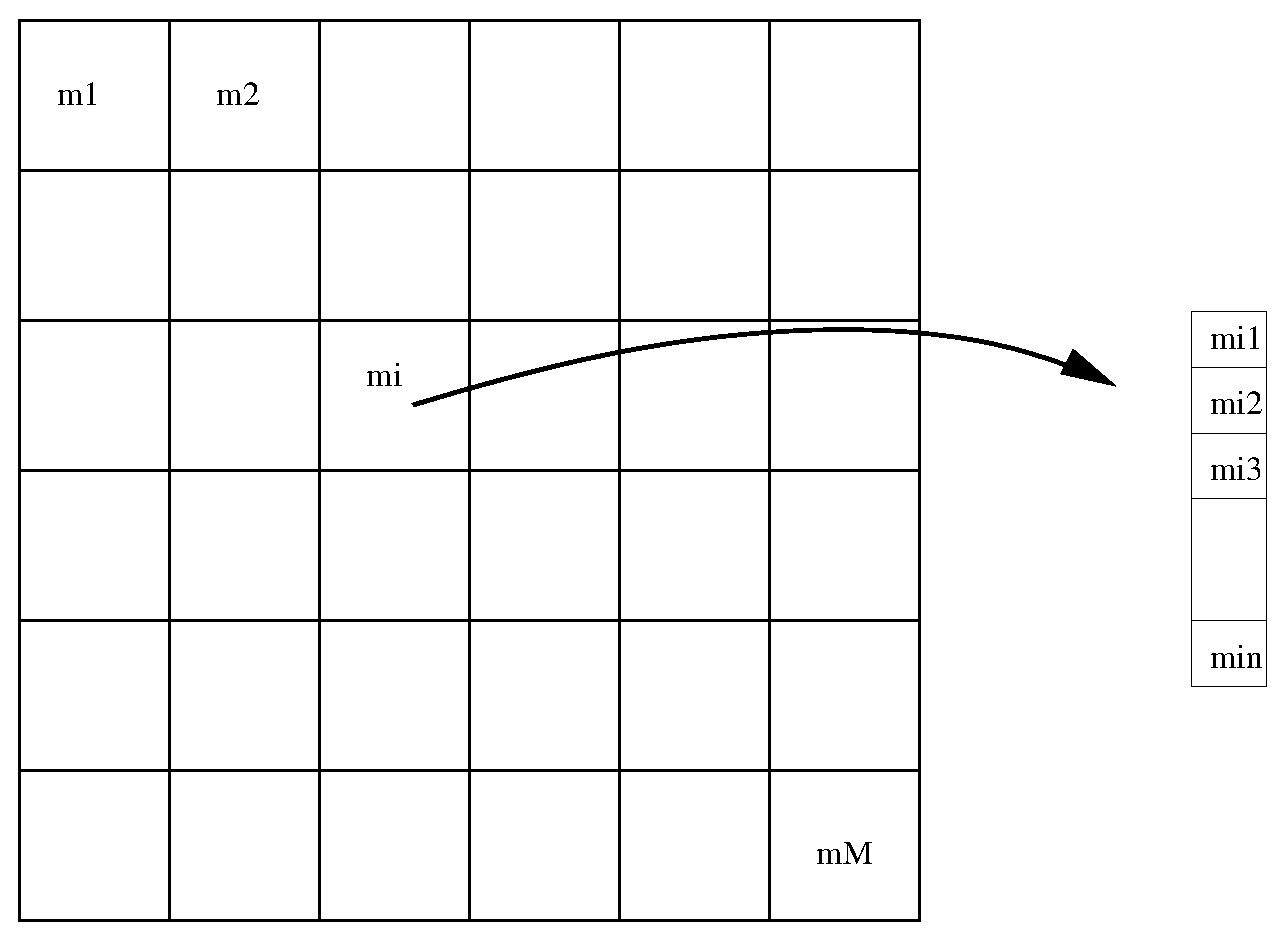
\includegraphics[width=0.45\textwidth]{carte.eps}
\itkcaption[Kohonen's Self Organizing Map]{Kohonen's Self Organizing Map}
\label{carte}
\end{figure}

A cell (or neuron) in the map is a good detector for a given input
vector $\underline x = \left[x_{1},x_{2},\cdots,x_{n}\right]^T\in
\mathbb{R}^n$ if the latter is {\em close} to the former. This
distance between vectors can be represented by the scalar product 
$\underline{x}^T\cdot\underline{m_i}$, but for most of the cases other
distances can be used, as for instance the Euclidean one. The cell
having the weight vector closest to the input vector is called the
{\em winner}.

%\subsubsection{Learning}
The goal of the learning step is to get a map which is representative
of an input example set. It is an iterative procedure which consists
in passing each input example to the map, testing the response of each
neuron and modifying the map to get it closer to the examples.

\begin{algo}
SOM learning:
\begin{enumerate}
\item $t=0$.
\item Initialize the weight vectors of the map (randomly, for instance).
\item While $t<$ number of iterations, do:
\begin{enumerate}
\item $k=0$.
\item While $k<$ number of examples, do:
\begin{enumerate}
\item Find the vector $\underline{m}_i(t)$ which minimizes the distance
$d(\underline{x}_k,\underline{m}_i(t))$
\item For a neighborhood $N_c(t)$ around the winner cell, apply the transformation:
\begin{equation}
\underline{m}_i(t+1)=\underline{m}_i(t)+\beta(t)\left[\underline{x}_k(t)-\underline{m}_i(t)\right]
\label{khoupdate}
\end{equation}
\item $k=k+1$
\end{enumerate}
\item $t=t+1$.
\end{enumerate}

\end{enumerate}
\end{algo}


In \ref{khoupdate}, $\beta(t)$ is a decreasing function with the
geometrical distance to the winner cell. For instance:
\begin{equation}
\beta(t)=\beta_0(t)e^{-\frac{\parallel \underline{r}_i -  \underline{r}_c\parallel^2}{\sigma^2(t)}},
\end{equation}
with $\beta_0(t)$ and $\sigma(t)$ decreasing functions with time and
$\underline{r}$ the cell coordinates in the output -- map -- space.\\

Therefore the algorithm consists in getting the map closer to the
learning set. The use of a neighborhood around the winner cell allows
the organization of the map into areas which specialize in the
recognition of different patterns. This neighborhood also ensures that
cells which are topologically close are also close in terms of the
distance defined in the feature space.


%%%1. Construction SOM
\subsubsection{Building a color table}
\label{sec:SOMColorTable}
\input{SOMExample}
\subsubsection{SOM Classification}
\label{sec:SOMClassification}
\input{SOMClassifierExample}

\subsubsection{Multi-band, streamed classification}

\ifitkFullVersion
\input{SOMImageClassificationExample.tex}
\fi

%%%2. Lecture SOM et ensemble de vecteurs autre image pour construire
%%%ActivationMAP 

%\subsection{Bayesian classification}

\subsection{Bayesian Plug-In Classifier}
\label{sec:BayesianPluginClassifier}

\ifitkFullVersion 
\input{BayesianPluginClassifier.tex}
\fi


\subsection{Expectation Maximization Mixture Model Estimation}
\label{sec:ExpectationMaximizationMixtureModelEstimation}

\ifitkFullVersion 
\input{ExpectationMaximizationMixtureModelEstimator.tex}
\fi




%%%%%%%%%%%%%%%%%%%%%%%%%%%%%%%%%%%%%%%%%%%%%%%%%%%%%%%%%%%%%%%%%%%%%%
\subsection{Statistical Segmentations}
\label{sec:StatisticalSegmentations}

%\subsection{Markov Random Fields}

\subsubsection{Stochastic Expectation Maximization}
\label{sec:SEM}

The Stochastic Expectation Maximization (SEM) approach is a stochastic 
version of the EM mixture estimation seen on
section~\ref{sec:ExpectationMaximizationMixtureModelEstimation}. It has been 
introduced by \cite{CeDi95} to prevent convergence of the EM approach from
local minima. It avoids the analytical maximization issued by integrating a
stochastic sampling procedure in the estimation process. It induces an almost
sure (a.s.) convergence to the algorithm.

From the initial two step formulation of the EM mixture estimation, the SEM
may be decomposed into 3 steps:
\begin{enumerate}
\item \textbf{E-step}, calculates the expected membership values for each 
measurement vector to each classes.
\item \textbf{S-step}, performs a stochastic sampling of the membership vector
to each classes, according to the membership values computed in the E-step.
\item \textbf{M-step}, updates the parameters of the membership probabilities
(parameters to be defined through the class
\subdoxygen{itk}{Statistics}{ModelComponentBase} and its inherited classes).
\end{enumerate}
The implementation of the SEM has been turned to a contextual SEM in the sense
where the evaluation of the membership parameters is conditioned to
membership values of the spatial neighborhood of each pixels.

\ifitkFullVersion 
\input{SEMModelEstimatorExample.tex}
\fi


%%%%%%%%%%%%%%%%%%%%%%%%%%%%%%%%%%%%%%%%%%%%%%%%%%%%%%%%%%%%%%%%%%%%%%

\subsection{Classification using Markov Random Fields}
\label{sec:MarkovRandomField}

Markov Random Fields are probabilistic models that use the statistical
dependency between
pixels in a neighborhood to infeer the value of a give pixel.

\subsubsection{ITK framework}
\label{sec:MarkovRandomFieldITK}
The
\subdoxygen{itk}{Statistics}{MRFImageFilter} uses the maximum a posteriori (MAP)
estimates for modeling the MRF. The object traverses the data set and uses the
model generated by the Mahalanobis distance classifier to get the the distance
between each pixel in the data set to a set of known classes, updates the
distances by evaluating the influence of its neighboring pixels (based on a MRF
model) and finally, classifies each pixel to the class which has the minimum
distance to that pixel (taking the neighborhood influence under consideration).
The energy function minimization is done using the iterated conditional modes
(ICM) algorithm \cite{Besag1986}.

\ifitkFullVersion
\input{ScalarImageMarkovRandomField1.tex}
\fi 

\subsubsection{OTB framework}
\label{sec:MarkovRandomFieldOTB}
The ITK approach was considered not to be flexible enough for some
remote sensing applications. Therefore, we decided to implement our
own framework.
\index{Markov}

\begin{figure}[th]
  \centering
  \includegraphics[width=0.7\textwidth]{MarkovFramework.eps}
  \itkcaption[OTB Markov Framework]{OTB Markov Framework.}
  \label{fig:markovFramework}
\end{figure}

\index{Markov!Classification}
\ifitkFullVersion
\input{MarkovClassification1Example.tex}
\fi 

\index{Markov!Classification}
\ifitkFullVersion
\input{MarkovClassification2Example.tex}
\fi 

\index{Markov!Classification}
\ifitkFullVersion
\input{MarkovClassification3Example.tex}
\fi 

\index{Markov!Regularization}
\ifitkFullVersion
\input{MarkovRegularizationExample.tex}
\fi 




\section{Supervised classification}

\subsection{Generic machine learning framework}
\label{sec:MLGenericFramework}

The OTB supervised classification is implemented as a generic Machine Learning 
framework, supporting several possible machine learning library as backends.
As of now both libSVM (the machine learning library historically integrated in OTB)
and the machin learning methods of OpenCV library (\cite{opencv_library}) are available.

The current list of classifiers available through the same generic interface within the OTB is:

\begin{itemize}
  \item \textbf{LibSVM}: Support Vector Machines classifier based on libSVM.
  \item \textbf{SVM}: Support Vector Machines classifier based on OpenCV, itself based on libSVM.
  \item \textbf{Bayes}: Normal Bayes classifier based on OpenCV.
  \item \textbf{Boost}: Boost classifier based on OpenCV.
  \item \textbf{DT}: Decision Tree classifier based on OpenCV.
  \item \textbf{RF}: Random Forests classifier based on the Random Trees in OpenCV.
  \item \textbf{GBT}: Gradient Boosted Tree classifier based on OpenCV.
  \item \textbf{KNN}: K-Nearest Neighbors classifier based on OpenCV.
  \item \textbf{ANN}: Artificial Neural Network classifier based on OpenCV.
\end{itemize}


\subsection{An example of supervised classification method: Support Vector Machines}
\label{sec:SupportVectorMachines}

\subsubsection{SVM general description}
Kernel based learning methods in general and the Support Vector
Machines (SVM) in particular, have been introduced in the last years
in learning theory for classification and regression tasks,
\cite{vapnik}. SVM have been successfully applied to text
categorization, \cite{joachims}, and face recognition,
\cite{osuna}. Recently, they have been successfully used for the
classification of hyperspectral remote-sensing images, \cite{bruzzoneSVM}.

Simply stated, the approach consists in searching for the separating
surface between 2 classes by the determination of the subset of
training samples which best describes the boundary between the 2
classes. These samples are called support vectors and completely
define the classification system. In the case where the two classes are
nonlinearly separable, the method uses a kernel expansion in order to make
projections of the feature space onto higher dimensionality spaces
where the separation of the classes becomes linear.


\subsubsection{SVM mathematical formulation}

This subsection reminds the basic principles of SVM learning and
classification. A good tutorial on SVM can be found in, \cite{burges}.
 
We have $N$ samples represented by the couple $(y_i,\mathbf{x}_i),
i=1\ldots N$ where $y_i \in \{-1,+1\}$ is the class label and
$\mathbf{x}_i \in \mathbb{R}^n$ is the feature vector of dimension
$n$. A classifier is a function  $$f(\mathbf{x},\boldsymbol{\alpha}) :
\mathbf{x}\mapsto y$$ where $\boldsymbol{\alpha}$ are the classifier
parameters. The SVM finds the optimal separating hyperplane which
fulfills the following constraints :
    \begin{itemize}
      \item The samples with labels $+1$ and $-1$ are on different
      sides of the hyperplane.
      \item The distance of the closest vectors to the hyperplane is
      maximised. These are the support vectors (SV) and this distance is
      called the margin.
    \end{itemize}

    The separating hyperplane has the equation
    $$\mathbf{w}\cdot\mathbf{x}+b=0;$$ with $\mathbf{w}$ being its
    normal vector and $x$ being any point of the hyperplane. The
    orthogonal distance to the origin is given by
    $\frac{|b|}{\|\mathbf{w}\|}$. Vectors located outside the
    hyperplane have either $\mathbf{w}\cdot\mathbf{x}+b>0$ or
      $\mathbf{w}\cdot\mathbf{x}+b<0$.

    Therefore, the classifier function can be written as
    $$f(\mathbf{x},\mathbf{w}, b)=sgn(\mathbf{w}\cdot\mathbf{x}+b).$$
    
The SVs are placed on two hyperplanes which are parallel to the
      optimal separating one. In order to find the optimal
      hyperplane, one sets $\mathbf{w}$ and
      $b$ : $$\mathbf{w}\cdot\mathbf{x}+b=\pm 1.$$

Since there must not be any vector inside the margin, the following
constraint can be used:
    $$\mathbf{w}\cdot\mathbf{x}_i+b\ge +1\text{ if }y_i=+1;$$
    $$\mathbf{w}\cdot\mathbf{x}_i+b\le -1\text{ if }y_i=-1;$$ which
    can be rewritten as $$y_i(\mathbf{w}\cdot\mathbf{x}_i+b)-1\ge 0~  ~ \forall i.$$

    The orthogonal distances of the 2 parallel hyperplanes to the
    origin are $\frac{|1-b|}{\|\mathbf{w}\|}$ and
      $\frac{|-1-b|}{\|\mathbf{w}\|}$. Therefore the modulus of the
    margin is equal to $\frac{2}{\|\mathbf{w}\|}$ and it has to be
    maximised.

    Thus, the problem to be solved is:

	\begin{itemize}
	\item Find $\mathbf{w}$ and $b$ which minimise
	 $\left\{ \frac{1}{2}\|\mathbf{w}\|^2 \right\}$
	\item under the constraint :
	 $y_i(\mathbf{w}\cdot\mathbf{x}_i+b)\ge 1~  ~ i=1\ldots N.$
	\end{itemize}

	This problem can be solved by using the Lagrange multipliers
	with one multiplier per sample. It can be shown that only the
	support vectors will have a positive Lagrange multiplier.

	In the case where the two classes are not exactly linearly
	separable, one can modify the constraints above by using 
      $$\mathbf{w}\cdot\mathbf{x}_i+b\ge +1 - \xi_i \text{ if }y_i=+1;$$
    $$\mathbf{w}\cdot\mathbf{x}_i+b\le -1+\xi_i \text{ if }y_i=-1;$$
    $$\xi_i\ge 0~  ~\forall i.$$

	If $\xi_i > 1$, one considers that the sample is wrong. The
	function which has then to be minimised is
	$\frac{1}{2}\|\mathbf{w}\|^2 + C\left( \sum_i \xi_i\right); $,
	where $C$ is a tolerance parameter. The optimisation problem
	is the same than in the linear case, but one multiplier has to
	be added for each new constraint $\xi_i\ge 0$.

	If the decision surface needs to be non-linear, this solution
	cannot be applied and the kernel approach has to be adopted.


One drawback of the SVM is that, in their basic version, they can only
solve two-class problems. Some works exist in the field of multi-class
SVM (see \cite{allwein00reducing,weston98multiclass}, and the
comparison made by \cite{hsu01comparison}), but they are
not used in our system.

You have to be aware that to achieve better convergence of the algorithm it is 
strongly advised to normalize feature vector components in the $[-1;1]$ 
interval.

For problems with $N > 2$ classes, one can choose either to train $N$
SVM (one class against all the others), or to train $N\times(N-1)$ SVM
(one class against each of the others). In the second approach, which
is the one that we use, the final decision is taken by choosing the
class which is most often selected by the whole set of SVM.



\subsection{Learning from samples}
\label{ssec:LearningFromSamples}
\input{TrainMachineLearningModelFromSamplesExample.tex}

\subsection{Learning from images}
\label{ssec:LearningFromImages}
\input{TrainMachineLearningModelFromImagesExample.tex}


%\subsection{Learning With PointSets}
%\label{sec:LearningWithPointSets}
%\input{SVMPointSetModelEstimatorExample}

%\subsection{PointSet Classification}
%\label{sec:PointSetClassification}
%\input{SVMPointSetClassificationExample}

%\subsection{Learning With Images}
%\label{sec:LearningWithImages}
%\input{SVMImageModelEstimatorExample}

%\subsection{Image Classification}
%\label{sec:ImageClassification}
%\input{SVMImageClassificationExample}
%\input{SVMImageEstimatorClassificationMultiExample}


\subsection{Multi-band, streamed classification}

\ifitkFullVersion
\input{SupervisedImageClassificationExample.tex}
\fi




\subsection{Generic Kernel SVM}
OTB has developed a specific interface for user-defined kernels. However, the 
following functions use a deprecated OTB interface. A function 
$k(\cdot,\cdot)$ is considered to be a kernel when:
\begin{align}\label{eqMercer}
        \forall g(\cdot) \in {\cal L}^2(\mathbbm{R}^n) \quad & \text{so 
that} \quad
        \int g(\boldsymbol{x})^2 d\boldsymbol{x} \text{ be finite,} \\
        & \text{then} \quad \int k(\boldsymbol{x},\boldsymbol{y}) \, 
g(\boldsymbol{x})
        \, g(\boldsymbol{y}) \, d\boldsymbol{x} d\boldsymbol{y} \geqslant 0,
        \notag
\end{align}
which is known as the {\em Mercer condition\/}.

When defined through the OTB, a kernel is a class that inherits from
\code{GenericKernelFunctorBase}. Several virtual functions have to 
be overloaded:
\begin{itemize}
\item The \code{Evaluate} function, which implements the behavior of the 
kernel
itself. For instance, the classical linear kernel could be re-implemented
with:
\begin{verbatim}
        double
        MyOwnNewKernel
        ::Evaluate ( const svm_node * x, const svm_node * y,
                     const svm_parameter & param ) const
        {
                return this->dot(x,y);
        }
\end{verbatim}
This simple example shows that the classical dot product is already 
implemented
into \subdoxygen{otb}{GenericKernelFunctorBase}{dot()} as a protected
function.
\item The \code{Update()} function which synchronizes local variables and 
their
integration into the initial SVM procedure. The following examples will show
the way to use it.
\end{itemize}

Some pre-defined generic kernels have already been implemented in OTB:
\begin{itemize}
\item \doxygen{otb}{MixturePolyRBFKernelFunctor} which implements a 
linear mixture
of a polynomial and a RBF kernel;
\item \doxygen{otb}{NonGaussianRBFKernelFunctor} which implements a non
gaussian RBF kernel;
\item \doxygen{otb}{SpectralAngleKernelFunctor}, a kernel that integrates
the Spectral Angle, instead of the Euclidean distance, into an inverse 
multiquadric kernel.
This kernel may be appropriated when using multispectral data.
\item \doxygen{otb}{ChangeProfileKernelFunctor}, a kernel which is
dedicated to the supervized classification of the multiscale change profile
presented in section \ref{sec:KullbackLeiblerProfile}.
\end{itemize}

\subsubsection{Learning with User Defined Kernels}
\label{sec:Learningwithuserdefinedkernel}
\ifitkFullVersion
\input{SVMGenericKernelImageModelEstimatorExample.tex}
\fi

\subsubsection{Classification with user defined kernel}

\ifitkFullVersion
\input{SVMGenericKernelImageClassificationExample.tex}
\fi




\section{Fusion of Classification maps}

\subsection{General approach of image fusion}
In order to obtain a relevant image classification it is sometimes necessary to 
fuse several classification maps coming from different classification methods 
(SVM, KNN, Random Forest, Artificial Neural Networks,...). The fusion of 
classification maps combines them in a more robust and precise one. Two methods are 
available in the OTB: the majority voting and the Demspter Shafer framework.


\subsection{Majority voting}
\subsubsection{General description}
For each input pixel, the Majority Voting method consists in choosing the more 
frequent class label among all classification maps to fuse. In case of not unique 
more frequent class labels, the undecided value is set for such pixels in 
the fused output image.

\subsubsection{An example of majority voting fusion}
\ifitkFullVersion
\input{MajorityVotingFusionOfClassificationMapsExample.tex}
\fi


\subsection{Dempster Shafer}

\subsubsection{General description}
A more adaptive fusion method using the 
\href{http://en.wikipedia.org/wiki/Dempster\%E2\%80\%93Shafer_theory}{Dempster-Shafer theory} 
is available within the OTB. This method is adaptive as it is based on the 
so-called belief function of each class label for each classification map. Thus, 
each classified pixel is associated to a degree of confidence according to the 
classifier used. In the Dempster Shafer framework, the expert's point of view 
(i.e. with a high belief function) is considered as the truth. In order to 
estimate the belief function of each class label, we use the Dempster Shafer 
combination of masses of belief for each class label and for each classification 
map. In this framework, the output fused label of each pixel is the one with the 
maximal belief function.

Like for the majority voting method, the Dempster Shafer fusion handles not 
unique class labels with the maximal belief function. In this case, the output 
fused pixels are set to the undecided value.

The confidence levels of all the class labels are estimated from a comparision of 
the classification maps to fuse with a ground truth, which results in a 
confusion matrix. For each classification maps, these confusion matrices are then 
used to estimate the mass of belief of each class label.


\subsubsection{Mathematical formulation of the combination algorithm}

A description of the mathematical formulation of the Dempster Shafer combination 
algorithm is available in the following OTB Wiki page:
\href{http://wiki.orfeo-toolbox.org/index.php/Information_fusion_framework}{http://wiki.orfeo-toolbox.org/index.php/} page.

\subsubsection{An example of Dempster Shafer fusion}
\ifitkFullVersion
\input{DempsterShaferFusionOfClassificationMapsExample.tex}
\fi



\section{Classification map regularization}

%\subsection{Regularization by neighborhood-based majority voting}

\ifitkFullVersion
\input{ClassificationMapRegularizationExample.tex}
\fi




\chapter{Image Visualization and output}
\label{chap:ImageVisualization}

After processing your images with OTB, you probably want to see the result. As it is quite straightforward in some situation, if can be a bit trickier in other. For example, some filters will give you a list of polygons as an output. Other can return an image with each region labelled by a unique index. In this section we are going to provide few examples to help you produce beautiful output ready to be included in your publications/presentations.


\section{Viewer}
Even if OTB is not a visualization toolkit as for instance VTK
(\emph{The Visualization Toolkit} \url{http://www.vtk.org}), some
simple functionalities for image visualization are given in the
toolbox. Indeed, for algorithm prototyping, it is sometimes more
useful to \emph{see} the result on the screen, than saving it to a
file and then open in with an external viewer.

OTB provides the \doxygen{otb}{ImageViewer} class which is compatible
with the pipeline and can therefore replace the
\doxygen{otb::ImageFileWriter} during proto-typing phases.

\input{VisuExample1.tex}


\section{Images}

\subsection{Grey Level Images}
\label{sec:ViewingGreyLevelImages}

\input{ScalingFilterExample.tex}

\subsection{Multiband Images}
\label{sec:ViewingMultibandImages}

\input{PrintableImageFilterExample.tex}

\subsection{Indexed Images}
\label{sec:ViewingIndexedImages}

\input{IndexedToRGBExample.tex}

\subsection{Altitude Images}
\label{sec:ViewingAltitudeImages}

\input{DEMToRainbowExample.tex}

\index{hill shading}
\input{HillShadingExample.tex}



%%% \chapter{Applications}
\label{sec:Applications}

This chapter introduces a set of ready-to-use applications. 
These applications were designed to perform  simple remote sensing tasks, 
more complex than simple examples, to demonstrate the use of the OTB 
functions. They were previously known as the OTB-Applications 
package but are now part of the OTB library. The new framework is 
slightly different from before but they can be used pretty much the 
same way: each application has its set of inputs, outputs, parameters. 
The applications can be lauched as a command line interface but also
via a Qt GUI. In addition, they can be wrapped for SWIG and PyQt. For a 
complete list of these applications, please refer to the 
\href{http://orfeo-toolbox.org/Applications}{applications documentation}.

\section{Example of use}
\label{sec:appExample}



\part{Developper's guide}
\chapter{Iterators}
\label{sec:ImageIteratorsChapter}
\index{Iterators!image|(}
\index{Generic Programming}
This chapter introduces the \emph{image iterator}, an important generic
programming construct for image processing in ITK.  An iterator is a
generalization of the familiar C programming language pointer used to
reference data in memory.  ITK has a wide variety of image iterators, some of
which are highly specialized to simplify common image processing tasks.

The next section is a brief introduction that defines iterators in the context
of ITK.  Section \ref{sec:IteratorsInterface} describes the programming
interface common to most ITK image iterators.
Sections~\ref{sec:ImageIterators}--\ref{sec:NeighborhoodIterators} document
specific ITK iterator types and provide examples of how they are used.

\section{Introduction}
\label{sec:IteratorsIntroduction}
% Further define iterators in the context of generic programming.
\index{generic programming}
\index{Iterators!definition of}
Generic programming models define functionally independent components called
\emph{containers} and \emph{algorithms}.  Container objects store data and
algorithms operate on data.  To access data in containers, algorithms use a
third class of objects called \emph{iterators}.  An iterator is an
abstraction of a memory pointer.  Every container type must define its own
iterator type, but all iterators are written to provide a common interface so
that algorithm code can reference data in a generic way and maintain
functional independence from containers.

The iterator is so named because it is used for \emph{iterative}, sequential
access of container values.  Iterators appear in \code{for} and
\code{while} loop constructs, visiting each data point in turn.  
A C pointer, for example, is a type of iterator.  It can be moved
forward (incremented) and backward (decremented) through memory to
sequentially reference elements of an array. Many iterator implementations
have an interface similar to a C pointer.

\index{Iterators!advantages of}
In ITK we use iterators to write generic image processing code for images
instantiated with different combinations of pixel type, pixel
container type, and dimensionality.  Because ITK image iterators are
specifically designed to work with \emph{image} containers, their interface and
implementation is optimized for image processing tasks.  Using the ITK
iterators instead of accessing data directly through the
\doxygen{otb}{Image} interface has many advantages. Code is more
compact and often generalizes automatically to higher dimensions, algorithms
run much faster, and iterators simplify tasks such as multithreading and
neighborhood-based image processing.


\section{Programming Interface}
\label{sec:IteratorsInterface}

\index{Iterators!programming interface|(}
%Creating iterators
This section describes the standard ITK image iterator programming interface.
Some specialized image iterators may deviate from this standard or provide
additional methods.

\subsection{Creating Iterators}
\label{sec:CreatingIterators}

\index{Iterators!construction of}
All image iterators have at least one template parameter that is the image
type over which they iterate.  There is no restriction on the dimensionality
of the image or on the pixel type of the image.

\index{Iterators!and image regions}

An iterator constructor requires at least two arguments, a smart pointer to the
image to iterate across, and an image region. The image region, called the
\emph{iteration region}, is a rectilinear area in which iteration is
constrained.  The iteration region must be wholly contained within the image.
More specifically, a valid iteration region is any subregion of the image
within the current \code{BufferedRegion}.  See Section~\ref{sec:ImageSection}
for more information on image regions.

\index{Iterators!const}
There is a const and a non-const version of most ITK image iterators. A
non-const iterator cannot be instantiated on a non-const image pointer.
Const versions of iterators may read, but may not write pixel values.

Here is a simple example that defines and constructs a simple image iterator
for an \doxygen{otb}{Image}.

\small
\begin{verbatim}
  typedef otb::Image<float, 3> ImageType;
  typedef itk::ImageRegionConstIterator< ImageType > ConstIteratorType;
  typedef itk::ImageRegionIterator< ImageType > IteratorType;

  ImageType::Pointer image = SomeFilter->GetOutput();

  ConstIteratorType constIterator( image, image->GetRequestedRegion() );
  IteratorType iterator( image, image->GetRequestedRegion() );
\end{verbatim}
\normalsize

\subsection{Moving Iterators}
\label{sec:MovingIterators}
An iterator is described as \emph{walking} its iteration region.  At any
time, the iterator will reference, or ``point to'', one pixel location in the
N-dimensional (ND) image.  \emph{Forward iteration} goes from the beginning
of the iteration region to the end of the iteration region.  \emph{Reverse
iteration}, goes from just past the end of the region back to the beginning.
There are two corresponding starting positions for iterators, the
\emph{begin} position and the \emph{end} position.  An iterator can be moved
directly to either of these two positions using the following methods.

\index{forward iteration}
\index{reverse iteration}
\index{iteration region}
\index{Iterators!GoToBegin()}

\begin{itemize}
\item \textbf{\code{GoToBegin()}} Points the iterator to the first valid
data element in the region.

\index{Iterators!GoToEnd()}
\item \textbf{\code{GoToEnd()}} Points the iterator to \emph{one position past}
the last valid element in the region.
\end{itemize}

Note that the end position is not actually located within the iteration region.  This is
important to remember because attempting to dereference an iterator at its end
position will have undefined results.

%Moving iteators
ITK iterators are moved back and forth across their iterations using the 
decrement and increment operators.

\index{Iterators!operator++()}
\begin{itemize}
\item \textbf{\code{operator++()}} Increments the iterator one position in the
positive direction.  Only the prefix increment operator is defined for ITK image
iterators.

\index{Iterators!operator--}
\item \textbf{\code{operator--()}} Decrements the iterator one position in the
negative direction.  Only the prefix decrement operator is defined for ITK
image iterators. 
\end{itemize}

Figure~\ref{fig:WalkingIterator} illustrates typical iteration over
an image region.  Most iterators increment and decrement in the direction of
the fastest increasing image dimension, wrapping to the first position in the
next higher dimension at region boundaries.  In other words, an
iterator first moves across columns, then down rows, then from slice to slice,
and so on.

\begin{figure}
\centering
\includegraphics[width=0.4\textwidth]{IteratorFigure1.eps}
\itkcaption[ITK image iteration]{Normal path of an iterator through a 
2D image.  The iteration region is shown in a darker shade.  An arrow denotes
a single iterator step, the result of one \code{++} operation.}
\protect\label{fig:WalkingIterator}
\end{figure}

In addition to sequential iteration through the image, some iterators may define
random access operators.  Unlike the increment operators, random access
operators may not be optimized for speed and require some knowledge of the
dimensionality of the image and the extent of the iteration region to use properly.

\begin{itemize}
\index{Iterators!operator+=()}
\item \textbf{\code{operator+=( OffsetType )}} Moves the iterator to the pixel
position at the current index plus specified \doxygen{itk}{Offset}.

\index{Iterators!operator-=()}
\item \textbf{\code{operator-=( OffsetType )}} Moves the iterator to 
the pixel position at the current index minus specified Offset.

\index{Iterators!SetPosition()}
\item \textbf{\code{SetPosition( IndexType )}} Moves the iterator to the given
\doxygen{itk}{Index} position.
\end{itemize}

The \code{SetPosition()} method may be extremely slow for more complicated
iterator types. In general, it should only be used for setting a starting
iteration position, like you would use \code{GoToBegin()} or \code{GoToEnd()}.

Some iterators do not follow a predictable path through their
iteration regions and have no fixed beginning or ending pixel
locations.  A conditional iterator, for example, visits pixels only if
they have certain values or connectivities.  Random iterators,
increment and decrement to random locations and may even visit a given
pixel location more than once.

%Testing for location
An iterator can be queried to determine if it is at the end or the beginning of
its iteration region. 

\begin{itemize}
\index{Iterators!IsAtEnd()}
\item \textbf{\code{bool IsAtEnd()}} True if the iterator points to \emph{one
position past} the end of the iteration region.

\index{Iterators!IsAtBegin()}
\item \textbf{\code{bool IsAtBegin()}} True if the iterator points to the first
position in the iteration region.  The method is typically used to test for the
end of reverse iteration.

\end{itemize}

An iterator can also report its current image index position.

\begin{itemize}
\index{Iterators!GetIndex()}
\item \textbf{\code{IndexType GetIndex()}} Returns the Index
of the image pixel that the iterator currently points to.
\end{itemize}

% A note on bounds checking
\index{Iterators!and bounds checking}
For efficiency, most ITK image iterators do not perform bounds checking.  It is
possible to move an iterator outside of its valid iteration region.
Dereferencing an out-of-bounds iterator will produce undefined results.

\subsection{Accessing Data}
\label{sec:AccessingData}
ITK image iterators define two basic methods for reading and writing pixel
values.

\begin{itemize}
\index{Iterators!Get()}
\item \textbf{\code{PixelType Get()}} Returns the value of the pixel at the
iterator position.

\index{Iterators!Set()}
\item \textbf{\code{void Set( PixelType )}} Sets the value of the pixel at the
iterator position.  Not defined for const versions of iterators.
\end{itemize}

% Describe efficiency due to inlining for all cases
The \code{Get()} and \code{Set()} methods are inlined and optimized
for speed so that their use is equivalent to dereferencing the image
buffer directly.  There are a few common cases, however, where using
\code{Get()} and \code{Set()} do incur a penalty. Consider the
following code, which fetches, modifies, and then writes a value back
to the same pixel location.

\small
\begin{verbatim}
  it.Set( it.Get() + 1 );
\end{verbatim}
\normalsize

As written, this code requires one more memory dereference than is necessary.
Some iterators define a third data access method that avoids this penalty.

\begin{itemize}
\index{Iterators!Value()}
\item \textbf{\code{PixelType \& Value()}} Returns a reference to the pixel at
the iterator position.
\end{itemize}

The \code{Value()} method can be used as either an lval or an rval in an
expression.  It has all the properties of \code{operator*}.  The
\code{Value()} method makes it possible to rewrite our example code more
efficiently.

\small
\begin{verbatim}
  it.Value()++;
\end{verbatim}
\normalsize

Consider using the \code{Value()} method instead of \code{Get()} or
\code{Set()} when a call to \code{operator=} on a pixel is non-trivial, such as
when working with vector pixels, and operations are done in-place in the
image. The disadvantage of using \code{Value} is that it cannot support image
adapters (see Section~\ref{sec:ImageAdaptors} on
page~\pageref{sec:ImageAdaptors} for more information about image adaptors).

\subsection{Iteration Loops}
\label{sec:IterationExample}
% Now give a psuedo code example for putting all of this together.
Using the methods described in the previous sections, we can now write a simple
example to do pixel-wise operations on an image.  The following code calculates
the squares of all values in an input image and writes them to an output image.

\small
\begin{verbatim}
  ConstIteratorType in( inputImage,   inputImage->GetRequestedRegion() );
  IteratorType out( outputImage, inputImage->GetRequestedRegion() );

  for ( in.GoToBegin(), out.GoToBegin(); !in.IsAtEnd(); ++in, ++out )
    {
    out.Set( in.Get() * in.Get() );
    }
\end{verbatim}
\normalsize

\index{Iterators!and image regions}
Notice that both the input and output iterators are initialized over the same
region, the \code{RequestedRegion} of \code{inputImage}.  This is good
practice because it ensures that the output iterator walks exactly the same set
of pixel indices as the input iterator, but does not require that the output
and input be the same size. The only requirement is that the input image
must contain a region (a starting index and size) that matches the
\code{RequestedRegion} of the output image.

\index{reverse iteration}
Equivalent code can be written by iterating through the image in reverse.
The syntax is slightly more awkward because the \emph{end} of the
iteration region is not a valid position and we can only test whether the
iterator is strictly \emph{equal} to its beginning position.  It is often more
convenient to write reverse iteration in a \code{while} loop.

\small
\begin{verbatim}
  in.GoToEnd();
  out.GoToEnd();
  while ( ! in.IsAtBegin() )
    {
    --in;
    --out;
    out.Set( in.Get() * in.Get() );
    }
\end{verbatim}
\normalsize

%\begin{itemize}
%\item \textbf{\code{operator==}}
%\item \textbf{\code{operator<}} 
%\item \textbf{\code{operator<=}}
%\item \textbf{\code{operator>}}
%\item \textbf{\code{operator>=}}
%\end{itemize}

%operator +=, -=, etc

% SetIndex()

% operator <, operator >, etc.

\index{Iterators!programming interface|)}
\section{Image Iterators}
\label{sec:ImageIterators}
%Introduction and overview
This section describes iterators that walk rectilinear image regions and
reference a single pixel at a time.  The \doxygen{itk}{ImageRegionIterator} is the
most basic ITK image iterator and the first choice for most applications. The
rest of the iterators in this section are specializations of
ImageRegionIterator that are designed make common image processing
tasks more efficient or easier to implement.

% Each of the iterators has a const and non-const version

\subsection{ImageRegionIterator}
\index{itk::ImageRegionIterator|(}
\label{sec:itkImageRegionIterator}
\input{ImageRegionIterator.tex}
\index{itk::ImageRegionIterator|)}

\subsection{ImageRegionIteratorWithIndex}
\label{sec:itkImageRegionIteratorWithIndex}
\index{itk::ImageRegionIteratorWithIndex|(}
\input{ImageRegionIteratorWithIndex.tex}
\index{itk::ImageRegionIteratorWithIndex|)}

\subsection{ImageLinearIteratorWithIndex}
\label{sec:itkImageLinearIteratorWithIndex}
\index{itk::ImageLinearIteratorWithIndex|(}
\input{ImageLinearIteratorWithIndex.tex}
%\input{ImageLinearIteratorWithIndex2.tex}
\index{itk::ImageLinearIteratorWithIndex|)}

%% \subsection{ImageSliceIteratorWithIndex}
%% \label{sec:itkImageSliceIteratorWithIndex}
%% \index{itk::ImageSliceIteratorWithIndex|(}
%% \input{ImageSliceIteratorWithIndex.tex}
%% \index{itk::ImageSliceIteratorWithIndex|)}

%% \subsection{ImageRandomConstIteratorWithIndex}
%% \label{sec:itkImageRandomConstIteratorWithIndex}
%% \index{itk::Image\-Random\-Const\-Iterator\-With\-Index|(}
%% \input{ImageRandomConstIteratorWithIndex}
%% \index{itk::Image\-Random\-Const\-Iterator\-With\-Index|)}

%\section{Conditional Iterators}
%\index{Iterators!conditional|(}
%\label{sec:ConditionalIterators}
%This section describes iterators that walk only pixels in an image region whose
%values satisfy a specified condition.  The condition is usually based on some
%function of the image values, such as comparing to a threshold.  When the
%condition function returns \code{true} at a pixel location, the iterator
%includes that location in its path.  The biggest use of these iterators is for
%walking non-rectilinear regions of interest, such as might be defined by
%implicit geometric shape functions or connected component regions.

%./Common/itkConditionalConstIterator.h (BaseClass)
%./Common/itkConditionalIterator.h (BaseClass)
%./Common/itkFloodFilledFunctionConditionalConstIterator.h (BaseClass)
%./Common/itkFloodFilledFunctionConditionalIterator.h (BaseClass)

%[ here are all classes where these filters are used:
% ./BasicFilters/itkConfidenceConnectedImageFilter.txx (ImageFunction)
% ./BasicFilters/itkConnectedThresholdImageFilter.txx (ImageFunction)
% ./BasicFilters/itkIsolatedConnectedImageFilter.txx (ImageFunction)
% ./BasicFilters/itkNeighborhoodConnectedImageFilter.txx (ImageFunction)
%
% ./Common/itkBinaryBallStructuringElement.txx (SpatialFunction)
% ./Common/itkBloxCoreAtomImage.txx (SpatialFunction)
% ./BasicFilters/itkBloxBoundaryPointToCoreAtomImageFilter.txx (SpatialFunction)
% ./BasicFilters/itkBloxBoundaryPointImageToBloxBoundaryProfileImageFilter.txx (SpatialFunction)
%]

%\subsection{itk::FloodFilledImageFunctionConditionalIterator}
%\label{itk::FloodFilledImageFunctionConditionalIterator}
%\index{itk::FloodFilledImageFunctionConditionalIterator|(}
%./Common/itkFloodFilledImageFunctionConditionalConstIterator.h
%./Common/itkFloodFilledImageFunctionConditionalIterator.h
%\index{itk::FloodFilledImageFunctionConditionalIterator|)}

%\subsection{itk::FloodFilledSpatialFunctionConditionalIterator}
%\label{itk::FloodFilledSpatialFunctionConditionalIterator}
%\index{itk::FloodFilledSpatialFunctionConditionalIterator|(}
%./Common/itkFloodFilledSpatialFunctionConditionalConstIterator.h
%./Common/itkFloodFilledSpatialFunctionConditionalIterator.h
%\index{itk::FloodFilledImageFunctionConditionalIterator|)}
%\index{Iterators!conditional|)}

\section{Neighborhood Iterators}
\label{sec:NeighborhoodIterators}
\index{Iterators!neighborhood|(}
In ITK, a pixel neighborhood is loosely defined as a small set of pixels that
are locally adjacent to one another in an image.  The size and shape
of a neighborhood, as well the connectivity among pixels in a neighborhood,
may vary with the application.

Many image processing algorithms are neighborhood-based, that is, the result at
a pixel $i$ is computed from the values of pixels in the ND neighborhood of
$i$. Consider finite difference operations in 2D.  A derivative at pixel index
$i = (j, k)$, for example, is taken as a weighted difference of the values
at $(j+1, k)$ and $(j-1, k)$. Other common examples of neighborhood operations
include convolution filtering and image morphology.

This section describes a class of ITK image iterators that are designed for
working with pixel neighborhoods. An ITK neighborhood iterator walks an image
region just like a normal image iterator, but instead of only referencing a
single pixel at each step, it simultaneously points to the entire ND
neighborhood of pixels.  Extensions to the standard iterator interface provide
read and write access to all neighborhood pixels and information
such as the size, extent, and location of the neighborhood.

Neighborhood iterators use the same operators defined in
Section~\ref{sec:IteratorsInterface} and the same code constructs as normal
iterators for looping through an
image. Figure~\ref{fig:NeighborhoodIteratorFig1} shows a neighborhood iterator
moving through an iteration region.  This iterator defines a $3x3$ neighborhood
around each pixel that it visits. The \emph{center} of the neighborhood
iterator is always positioned over its current index and all other neighborhood
pixel indices are referenced as offsets from the center index.  The pixel
under the center of the neighborhood iterator and all pixels under the shaded
area, or \emph{extent}, of the iterator can be dereferenced.



\begin{figure}
\centering
\includegraphics[width=0.6\textwidth]{NeighborhoodIteratorFig1.eps}
\itkcaption[Neighborhood iterator]{Path of a $3x3$ neighborhood
iterator through a 2D image region.  The extent of the neighborhood is
indicated by the hashing around the iterator position. Pixels that lie within
this extent are accessible through the iterator.  An arrow denotes a single
iterator step, the result of one \code{++} operation.}
\protect\label{fig:NeighborhoodIteratorFig1}
\end{figure}

\index{Neighborhood iterators!construction of}
\index{Neighborhood iterators!radius of}

In addition to the standard image pointer and iteration region
(Section~\ref{sec:IteratorsInterface}), neighborhood iterator constructors
require an argument that specifies the extent of the neighborhood to cover.
Neighborhood extent is symmetric across its center in each
axis and is given as an array of $N$ distances that are collectively called the
\emph{radius}. Each element $d$ of the radius, where $0 < d < N$ and
$N$ is the dimensionality of the neighborhood, gives the extent of the
neighborhood in pixels for dimension $N$.  The length of each face of the
resulting ND hypercube is $2d + 1$ pixels, a distance of $d$ on either side of
the single pixel at the neighbor center.
Figure~{\ref{fig:NeighborhoodIteratorFig2} shows the relationship between the
radius of the iterator and the size of the neighborhood for a variety of 2D
iterator shapes.

The radius of the neighborhood iterator is queried after construction
by calling the \code{GetRadius()} method.  Some other methods provide
some useful information about the iterator and its underlying image.

\begin{figure}
\centering
\includegraphics[width=0.9\textwidth]{NeighborhoodIteratorFig2.eps}
\itkcaption[Some possible neighborhood iterator shapes]{Several possible 2D
neighborhood iterator shapes are shown along with their radii and sizes.  A
neighborhood pixel can be dereferenced by its integer index (top) or its
offset from the center (bottom).  The center pixel of each iterator is
shaded.}
\protect\label{fig:NeighborhoodIteratorFig2}
\end{figure}

\begin{itemize}

\index{NeighborhoodIterator!GetRadius()}
\item \textbf{\code{SizeType GetRadius()}} Returns the ND radius of the
neighborhood as an \doxygen{itk}{Size}.

\index{NeighborhoodIterator!GetImagePointer()}
\item \textbf{\code{const ImageType *GetImagePointer()}} Returns the pointer to
the image referenced by the iterator.

\index{NeighborhoodIterator!Size()}
\item \textbf{\code{unsigned long Size()}} Returns the size in number of 
pixels of the neighborhood.

\end{itemize}

The neighborhood iterator interface extends the normal ITK iterator interface
for setting and getting pixel values.  One way to dereference pixels is to
think of the neighborhood as a linear array where each pixel has a unique
integer index. The index of a pixel in the array is determined by incrementing
from the upper-left-forward corner of the neighborhood along the fastest
increasing image dimension: first column, then row, then slice, and so on.  In
Figure~\ref{fig:NeighborhoodIteratorFig2}, the unique integer index is shown
at the top of each pixel.  The center pixel is always at position $n/2$, where
$n$ is the size of the array.

\begin{itemize}

\index{NeighborhoodIterator!GetPixel()}
\item \textbf{\code{PixelType GetPixel(const unsigned int i)}} Returns the 
value of the pixel at neighborhood position \code{i}.

\index{NeighborhoodIterator!SetPixel()}
\item \textbf{\code{void SetPixel(const unsigned int i, PixelType p)}} 
Sets the value of the pixel at position \code{i} to \code{p}.

\end{itemize}

Another way to think about a pixel location in a neighborhood is as an
ND offset from the neighborhood center.  The upper-left-forward corner
of a $3x3x3$ neighborhood, for example, can be described by offset
$(-1, -1, -1)$.  The bottom-right-back corner of the same neighborhood
is at offset $(1, 1, 1)$.  In
Figure~\ref{fig:NeighborhoodIteratorFig2}, the offset from center is
shown at the bottom of each neighborhood pixel.

\begin{itemize}

\index{NeighborhoodIterator!GetPixel()}
\item \textbf{\code{PixelType GetPixel(const OffsetType \&o)}} Get the value of
the pixel at the position offset \code{o} from the neighborhood center.

\index{NeighborhoodIterator!SetPixel()}
\item \textbf{\code{void SetPixel(const OffsetType \&o, PixelType p)}} Set
the value at the position offset \code{o} from the neighborhood center to
the value \code{p}.

\end{itemize}

The neighborhood iterators also provide a shorthand for setting and getting the
value at the center of the neighborhood.

\index{NeighborhoodIterators!}
\begin{itemize}

\index{NeighborhoodIterator!GetCenterPixel()}
\item \textbf{\code{PixelType GetCenterPixel()}} Gets the value at the center
of the neighborhood.

\index{NeighborhoodIterator!SetCenterPixel()}
\item \textbf{\code{void SetCenterPixel(PixelType p)}} Sets the value at the
center of the neighborhood to the value \code{p}

\end{itemize}

There is another shorthand for setting and getting values for pixels that
lie some integer distance from the neighborhood center along one of the image
axes.

\index{NeighborhoodIterators!}
\begin{itemize}

\index{NeighborhoodIterator!GetNext()}
\item \textbf{\code{PixelType GetNext(unsigned int d)}} Get the value
immediately adjacent to the neighborhood center in the positive direction along
the \code{d} axis.

\index{NeighborhoodIterator!SetNext()}
\item \textbf{\code{void SetNext(unsigned int d, PixelType p)}} Set the value
immediately adjacent to the neighborhood center in the positive direction along
the \code{d} axis to the value \code{p}.

\index{NeighborhoodIterator!GetPrevious()}
\item \textbf{\code{PixelType GetPrevious(unsigned int d)}} Get the value
immediately adjacent to the neighborhood center in the negative direction along
the \code{d} axis.

\index{NeighborhoodIterator!SetPrevious()}
\item \textbf{\code{void SetPrevious(unsigned int d, PixelType p)}}
Set the value immediately adjacent to the neighborhood center in the
negative direction along the \code{d} axis to the value \code{p}.

\item \textbf{\code{PixelType GetNext(unsigned int d, unsigned int
s)}} Get the value of the pixel located \code{s} pixels from the
neighborhood center in the positive direction along the \code{d} axis.

\item \textbf{\code{void SetNext(unsigned int d, unsigned int s, PixelType p)}}
Set the value of the pixel located \code{s} pixels from the neighborhood center
in the positive direction along the \code{d} axis to value \code{p}.

\item \textbf{\code{PixelType GetPrevious(unsigned int d, unsigned int
s)}} Get the value of the pixel located \code{s} pixels from the
neighborhood center in the positive direction along the \code{d} axis.
 
\item \textbf{\code{void SetPrevious(unsigned int d, unsigned int s,
PixelType p)}} Set the value of the pixel located \code{s} pixels from
the neighborhood center in the positive direction along the \code{d}
axis to value \code{p}.

\end{itemize}

It is also possible to extract or set all of the neighborhood values
from an iterator at once using a regular ITK neighborhood object.
This may be useful in algorithms that perform a particularly large
number of calculations in the neighborhood and would otherwise require
multiple dereferences of the same pixels.

\begin{itemize}

\index{NeighborhoodIterator!GetNeighborhood()}
\index{NeighborhoodIterator!SetNeighborhood()}
\item \textbf{\code{NeighborhoodType GetNeighborhood()}} Return a
\doxygen{itk}{Neighborhood} of the same size and shape as the neighborhood
iterator and contains all of the values at the iterator position.

\item \textbf{\code{void SetNeighborhood(NeighborhoodType \&N)}} Set all
of the values in the neighborhood at the iterator position to those contained
in Neighborhood \code{N}, which must be the same size and shape as the
iterator.

\end{itemize}

Several methods are defined to provide information about the neighborhood.

\index{NeighborhoodIterators!}
\begin{itemize}

\index{NeighborhoodIterator!GetIndex()}
\item \textbf{\code{IndexType GetIndex()}} Return the image
index of the center pixel of the neighborhood iterator.

\item \textbf{\code{IndexType GetIndex(OffsetType o)}} Return the
image index of the pixel at offset \code{o} from the neighborhood 
center.

\item \textbf{\code{IndexType GetIndex(unsigned int i)}} Return the
image index of the pixel at array position \code{i}.

\index{NeighborhoodIterator!GetOffset()}
\item \textbf{\code{OffsetType GetOffset(unsigned int i)}}  Return the offset
from the neighborhood center of the pixel at array position \code{i}.

\index{NeighborhoodIterator!GetNeighborhoodIndex()}
\item \textbf{\code{unsigned long GetNeighborhoodIndex(OffsetType o)}}
Return the array position of the pixel at offset \code{o} from the
neighborhood center.

\index{NeighborhoodIterator!GetSlice()}
\item \textbf{\code{std::slice GetSlice(unsigned int n)}} Return a
\code{std::slice} through the iterator neighborhood along axis \code{n}.

\end{itemize}

\index{Neighborhood iterators!boundary conditions}
\index{Neighborhood iterators!bounds checking}
A neighborhood-based calculation in a neighborhood close to an image
boundary may require data that falls outside the boundary.  The
iterator in Figure~\ref{fig:NeighborhoodIteratorFig1}, for example, is
centered on a boundary pixel such that three of its neighbors actually
do not exist in the image.  When the extent of a neighborhood falls
outside the image, pixel values for missing neighbors are supplied
according to a rule, usually chosen to satisfy the numerical
requirements of the algorithm.  A rule for supplying out-of-bounds
values is called a \emph{boundary condition}.
 
ITK neighborhood iterators automatically detect out-of-bounds dereferences and
will return values according to boundary conditions.  The boundary condition
type is specified by the second, optional template parameter of the iterator.
By default, neighborhood iterators use a Neumann condition where the first
derivative across the boundary is zero.  The Neumann rule simply returns the
closest in-bounds pixel value to the requested out-of-bounds location.  Several
other common boundary conditions can be found in the ITK toolkit.  They include
a periodic condition that returns the pixel value from the opposite side of the
data set, and is useful when working with periodic data such as Fourier
transforms, and a constant value condition that returns a set value $v$ for all
out-of-bounds pixel dereferences.  The constant value condition is equivalent
to padding the image with value $v$.

Bounds checking is a computationally expensive operation because it occurs each
time the iterator is incremented.  To increase efficiency, a neighborhood
iterator automatically disables bounds checking when it detects that it is
not necessary.  A user may also explicitly disable or enable bounds checking.
Most neighborhood based algorithms can minimize the need for bounds checking
through clever definition of iteration regions.  These techniques are explored
in Section~\ref{sec:NeighborhoodExample3}.

\begin{itemize}

\index{NeighborhoodIterator!NeedToUseBoundaryConditionOn()}
\item \textbf{\code{void NeedToUseBoundaryConditionOn()}} Explicitly turn
bounds checking on.  This method should be used with caution because
unnecessarily enabling bounds checking may result in a significant performance
decrease. In general you should allow the iterator to automatically determine
this setting.

\index{NeighborhoodIterator!NeedToUseBoundaryConditionOff()}
\item \textbf{\code{void NeedToUseBoundaryConditionOff()}} Explicitly disable
bounds checking. This method should be used with caution because disabling
bounds checking when it is needed will result in out-of-bounds reads and
undefined results.

\index{NeighborhoodIterator!OverrideBoundaryCondition()}
\item \textbf{\code{void OverrideBoundaryCondition(BoundaryConditionType *b)}} 
Overrides the templated boundary condition, using boundary condition
object \code{b} instead. Object \code{b} should not be deleted until
it has been released by the iterator.  This method can be used to
change iterator behavior at run-time.

\index{NeighborhoodIterator!ResetBoundaryCondition()}
\item \textbf{\code{void ResetBoundaryCondition()}} Discontinues the use of any
run-time specified boundary condition and returns to using the condition
specified in the template argument.

\index{NeighborhoodIterator!SetPixel()}
\item \textbf{\code{void SetPixel(unsigned int i, PixelType p, bool
status)}} Sets the value at neighborhood array position \code{i} to value
\code{p}.  If the position \code{i} is out-of-bounds, \code{status} is set to
\code{false}, otherwise \code{status} is set to \code{true}.
\end{itemize}

The following sections describe the two ITK neighborhood iterator classes,
\doxygen{itk}{NeighborhoodIterator} and \doxygen{itk}{ShapedNeighborhoodIterator}.
Each has a const and a non-const version.  The shaped iterator is a refinement
of the standard NeighborhoodIterator that supports an
arbitrarily-shaped (non-rectilinear) neighborhood.

\subsection{NeighborhoodIterator}
\label{sec:itkNeighborhoodIterator}

\index{NeighborhoodIterator!examples}
\index{Neighborhood iterators!examples}
The standard neighborhood iterator class in ITK is the
\doxygen{itk}{NeighborhoodIterator}.  Together with its \code{const} version,
\doxygen{itk}{ConstNeighborhoodIterator}, it implements the complete API
described above.  This section provides several examples to illustrate the use
of NeighborhoodIterator.

\index{edge detection}
\index{Sobel operator}
\subsubsection{Basic neighborhood techniques: edge detection}
\label{sec:NeighborhoodExample1}
\input{NeighborhoodIterators1.tex}

\index{convolution filtering}
\index{Sobel operator}
\subsubsection{Convolution filtering: Sobel operator}
\label{sec:NeighborhoodExample2}
\input{NeighborhoodIterators2.tex}

\subsubsection{Optimizing iteration speed}
\label{sec:NeighborhoodExample3}
\input{NeighborhoodIterators3.tex}

\index{Gaussian blurring}
\subsubsection{Separable convolution: Gaussian filtering}
\label{sec:NeighborhoodExample4}
\input{NeighborhoodIterators4.tex}

%% \subsubsection{Slicing the neighborhood}
%% \label{sec:NeighborhoodExample5}
%% \input{NeighborhoodIterators5.tex}

\subsubsection{Random access iteration}
\label{sec:NeighborhoodExample6}
\input{NeighborhoodIterators6.tex}

%./Common/itkConstNeighborhoodIterator.h
%./Common/itkNeighborhoodIterator.h

% Example1: Edge detection using ``hand-coded'' Sobel operator
% Example2: Sobel edge detection using convolution filtering and Sobel operator
% Example3: Improving boundary condition efficiency
% Example4: gaussian filtering, separable convolution
% Example5: Slicing the neighborhood: gaussian filtering, separable convolution
% Example6: Advanced Neighborhood Techniques: local minima, local maxima

\subsection{ShapedNeighborhoodIterator}
\label{sec:itkShapedNeighborhoodIterator}
\index{ShapedNeighborhoodIterator}
\index{Neighborhood iterators!shaped}
\index{Neighborhood iterators!as stencils}
This section describes a variation on the neighborhood iterator called a
\emph{shaped} neighborhood iterator.  A shaped neighborhood is defined like
a bit mask, or \emph{stencil}, with different offsets in the rectilinear
neighborhood of the normal neighborhood iterator turned off or on to create a
pattern.  Inactive positions (those not in the stencil) are not updated during
iteration and their values cannot be read or written.  The shaped iterator is
implemented in the class \doxygen{itk}{ShapedNeighborhoodIterator}, which is a
subclass of
\doxygen{itk}{NeighborhoodIterator}.  A const version,
\doxygen{itk}{ConstShapedNeighborhoodIterator}, is also available.

\index{Neighborhood iterators!active neighbors}
\index{Neighborhood iterators!inactive neighbors}
Like a regular neighborhood iterator, a shaped neighborhood iterator must be
initialized with an ND radius object, but the radius of the neighborhood of a
shaped iterator only defines the set of \emph{possible} neighbors.  Any number
of possible neighbors can then be activated or deactivated.  The shaped
neighborhood iterator defines an API for activating neighbors.  When a neighbor
location, defined relative to the center of the neighborhood, is activated, it
is placed on the \emph{active list} and is then part of the stencil.  An
iterator can be ``reshaped'' at any time by adding or removing offsets from the
active list.

\begin{itemize}

\index{ShapedNeighborhoodIterator!ActivateOffset()}
\item \textbf{\code{void ActivateOffset(OffsetType \&o)}} Include the offset
\code{o} in the stencil of active neighborhood positions.  Offsets are relative
to the neighborhood center.

\index{ShapedNeighborhoodIterator!DeactivateOffset()}
\item \textbf{\code{void DeactivateOffset(OffsetType \&o)}} Remove the offset
\code{o} from the stencil of active neighborhood positions.  Offsets are
relative to the neighborhood center. 

\index{ShapedNeighborhoodIterator!ClearActiveList()}
\item \textbf{\code{void ClearActiveList()}} Deactivate all positions in the
iterator stencil by clearing the active list.

\index{ShapedNeighborhoodIterator!GetActiveIndexListSize()}
\item \textbf{\code{unsigned int GetActiveIndexListSize()}} Return the number
of pixel locations that are currently active in the shaped iterator stencil.

\end{itemize}

Because the neighborhood is less rigidly defined in the shaped iterator, the
set of pixel access methods is restricted.  Only the \code{GetPixel()} and
\code{SetPixel()} methods are available, and calling these methods on an 
inactive neighborhood offset will return undefined results.

For the common case of traversing all pixel offsets in a neighborhood, the
shaped iterator class provides an iterator through the active offsets in its
stencil.   This \emph{stencil iterator} can be incremented or decremented and
defines \code{Get()} and \code{Set()} for reading and writing the values in the
neighborhood.

\begin{itemize}
\index{ShapedNeighborhoodIterator!Iterator::Begin()}
\item \textbf{\code{ShapedNeighborhoodIterator::Iterator Begin()}} Return a
const or non-const iterator through the shaped iterator stencil that points to
the first valid location in the stencil.

\index{ShapedNeighborhoodIterator!Iterator::End()}
\item \textbf{\code{ShapedNeighborhoodIterator::Iterator End()}} Return a
const or non-const iterator through the shaped iterator stencil that points
\emph{one position past} the last valid location in the stencil.
\end{itemize}

The functionality and interface of the shaped neighborhood iterator is best
described by example.  We will use the ShapedNeighborhoodIterator to
implement some binary image morphology algorithms (see \cite{Gonzalez1993},
\cite{Castleman1996}, et al.).  The examples that follow implement erosion and
dilation.

\index{ShapedNeighborhoodIterator!examples of}
\subsubsection{Shaped neighborhoods: morphological operations}
\label{sec:ShapedNeighborhoodExample}
\input{ShapedNeighborhoodIterators1.tex}
\input{ShapedNeighborhoodIterators2.tex}

%./Common/itkConstShapedNeighborhoodIterator.h
%./Common/itkShapedNeighborhoodIterator.h

\index{Iterators!neighborhood|)}

% ADD A SECTION WITH TIPS, SUGGESTIONS ON USING ITERATORS?  EXTENDING ITERATORS?
% USING ITERATORS FOR MULTITHREADING EXAMPLE?
\index{Iterators!image|)}


\chapter{Image Adaptors}
\label{sec:ImageAdaptors}

\index{ImageAdaptors}

\begin{figure}
\center
\includegraphics[width=0.8\textwidth]{ImageAdaptorConcept.eps}
\itkcaption[ImageAdaptor concept]{ The difference between using a
CastImageFilter and an ImageAdaptor.  ImageAdaptors
convert pixel values when they are accessed by iterators.  Thus, they do not
produces an intermediate image.  In the example
illustrated by this figure, the \emph{Image Y} is not created by the
ImageAdaptor; instead, the image is simulated on the fly each time an
iterator from the filter downstream attempts to access the image data.}
\label{fig:ImageAdaptorConcept}
\end{figure}

The purpose of an \emph{image adaptor} is to make one image appear
like another image, possibly of a different pixel type.  A typical
example is to take an image of pixel type \code{unsigned char} and
present it as an image of pixel type \code{float}. The motivation for
using image adaptors in this case is to avoid the extra memory
resources required by using a casting filter.  When we use the
\doxygen{itk}{CastImageFilter} for the conversion, the filter creates a
memory buffer large enough to store the \code{float} image. The
\code{float} image requires four times the memory of the
original image and contains no useful additional information. Image
adaptors, on the other hand, do not require the extra memory as
pixels are converted only when they are read using image iterators
(see Chapter~\ref{sec:ImageIteratorsChapter}).

Image adaptors are particularly useful when there is infrequent pixel access,
since the actual conversion occurs on the fly during the access operation. In
such cases the use of image adaptors may reduce overall computation time as
well as reduce memory usage. The use of image adaptors, however, can be
disadvantageous in some situations. For example, when the downstream filter
is executed multiple times, a CastImageFilter will cache its output after the
first execution and will not re-execute when the filter downstream is
updated. Conversely, an image adaptor will compute the cast every time.

Another application for image adaptors is to perform lightweight
pixel-wise operations replacing the need for a filter. In the toolkit,
adaptors are defined for many single valued and single parameter
functions such as trigonometric, exponential and logarithmic
functions. For example,
\begin{itemize}
\item \doxygen{itk}{ExpImageAdaptor}
\item \doxygen{itk}{SinImageAdaptor}
\item \doxygen{itk}{CosImageAdaptor}
\end{itemize}

The following examples illustrate common applications of image adaptors.

\section{Image Casting}
\label{sec:ImageAdaptorForBasicCasting}
\input{ImageAdaptor1.tex}

\section{Adapting RGB Images}
\label{sec:ImageAdaptorForRGB}
\input{ImageAdaptor2.tex}


\section{Adapting Vector Images}
\label{sec:ImageAdaptorForVectors}
\input{ImageAdaptor3.tex}

\section{Adaptors for Simple Computation}
\label{sec:ImageAdaptorForSimpleComputation}
\input{ImageAdaptor4.tex}


\section{Adaptors and Writers}

Image adaptors will not behave correctly when connected directly to a writer.
The reason is that writers tend to get direct access to the image buffer from
their input, since image adaptors do not have a real buffer their behavior in
this circumstances is incorrect. You should avoid instantiating the
\code{ImageFileWriter} or the \code{ImageSeriesWriter} over an image adaptor
type.


\chapter{How To Write A Filter}
\label{chapter:WriteAFilter}

This purpose of this chapter is help developers create their own
filter (process object).  This chapter is divided into four major
parts. An initial definition of terms is followed by an overview of
the filter creation process. Next, data streaming is discussed. The
way data is streamed in ITK must be understood in order to write
correct filters. Finally, a section on multithreading describes what
you must do in order to take advantage of shared memory parallel
processing.

\section{Terminology}
\label{sec:Terminology}

The following is some basic terminology for the discussion that follows.
Chapter \ref{chapter:SystemOverview} provides additional background
information.

\begin{itemize}
        \item The \textbf{data processing pipeline} is a directed graph of
        \textbf{process} and \textbf{data objects}. The pipeline inputs,
        operators on, and outputs data.
        \index{data processing pipeline}
        \index{process object}
        \index{data object}

        \item A \textbf{filter}, or \textbf{process object}, has one or more
        inputs, and one or more outputs.
        \index{filter}

        \item A \textbf{source}, or source process object, initiates the data
        processing pipeline, and has one or more outputs.
        \index{source}

        \item A \textbf{mapper}, or mapper process object, terminates the
        data processing pipeline. The mapper has one or more outputs, and may
        write data to disk, interface with a display system, or interface to
        any other system.
        \index{mapper}

        \item A \textbf{data object} represents and provides access to
        data. In ITK, the data object (ITK class \doxygen{itk}{DataObject}) is 
        typically of type \doxygen{otb}{Image} or \doxygen{itk}{Mesh}.
        \index{data object}

        \item A \textbf{region} (ITK class \doxygen{itk}{Region}) represents a 
        piece, or subset of the entire data set.
        \index{region}

        \item An \textbf{image region} (ITK class \doxygen{itk}{ImageRegion})
        represents a structured portion of data. ImageRegion is implemented
        using the \doxygen{itk}{Index} and \doxygen{itk}{Size} classes
        \index{image region}

        \item A \textbf{mesh region} (ITK class \doxygen{itk}{MeshRegion}) 
        represents an unstructured portion of data.
        \index{mesh region}

        \item The \textbf{LargestPossibleRegion} is the theoretical single,
        largest piece (region) that could represent the entire dataset. The
        LargestPossibleRegion is used in the system as the measure of the
        largest possible data size.
        \index{LargestPossibleRegion}

        \item The \textbf{BufferedRegion} is a contiguous block of memory
        that is less than or equal to in size to the
        LargestPossibleRegion. The buffered region is what has actually been
        allocated by a filter to hold its output.
        \index{BufferedRegion}

        \item The \textbf{RequestedRegion} is the piece of the dataset that a
        filter is required to produce. The RequestedRegion is less than or
        equal in size to the BufferedRegion. The RequestedRegion may differ
        in size from the BufferedRegion due to performance reasons. The
        RequestedRegion may be set by a user, or by an application that needs
        just a portion of the data.
        \index{RequestedRegion}

        \item The \textbf{modified time} (represented by ITK class
        \doxygen{itk}{TimeStamp}) is a monotonically increasing integer value that
        characterizes a point in time when an object was last modified.
        \index{modified time}

        \item \textbf{Downstream} is the direction of dataflow, from sources
        to mappers.
        \index{pipeline!downstream}

        \item \textbf{Upstream} is the opposite of downstream, from mappers
        to sources.
        \index{pipeline!upstream}

        \item The \textbf{pipeline modified time} for a particular data
        object is the maximum modified time of all upstream data objects and
        process objects.
        \index{pipeline!modified time}

        \item The term \textbf{information} refers to metadata that
        characterizes data. For example, index and dimensions are information
        characterizing an image region.
        \index{pipeline!information}
\end{itemize}

\section{Overview of Filter Creation}
\label{sec:OverviewFilterCreation}
\index{filter!overview of creation}

\itkpiccaption[Relationship between DataObjects and ProcessObjects]
{Relationship between DataObject and ProcessObject.
\label{fig:DataPipeLineOneConnection}}
\parpic(7cm,2.5cm)[r]{\includegraphics[width=6cm]{DataPipelineOneConnection.eps}}


Filters are defined with respect to the type of data they input (if
any), and the type of data they output (if any). The key to writing a
ITK filter is to identify the number and types of input and
output. Having done so, there are often superclasses that simplify
this task via class derivation. For example, most filters in ITK take
a single image as input, and produce a single image on output. The
superclass \doxygen{itk}{ImageToImageFilter} is a convenience class that
provide most of the functionality needed for such a filter.

Some common base classes for new filters include:

\begin{itemize}

  \item \code{ImageToImageFilter}: the most common filter base for
    segmentation algorithms.  Takes an image and produces a new image, by
    default of the same dimensions.  Override
    \code{GenerateOutputInformation} to produce a different size.

  \item \code{UnaryFunctorImageFilter}: used when defining a filter that
  applies a function to an image.

  \item \code{BinaryFunctorImageFilter}: used when defining a filter that
  applies an operation to two images.

  \item \code{ImageFunction}: a functor that can be applied to an image,
  evaluating $f(x) $ at each point in the image.

  \item \code{MeshToMeshFilter}: a filter that transforms meshes, such as
  tessellation, polygon reduction, and so on.

  \item \code{LightObject}: abstract base for filters that don't fit well
  anywhere else in the class hierarchy.  Also useful for ``calculator''
  filters; ie. a sink filter that takes an input and calculates a result
  which is retrieved using a \code{Get()} method.

\end{itemize}

Once the appropriate superclass is identified, the filter writer
implements the class defining the methods required by most all ITK
objects: \code{New()}, \code{PrintSelf()}, and protected constructor,
copy constructor, delete, and operator=, and so on. Also, don't forget
standard typedefs like \code{Self}, \code{Superclass}, \code{Pointer}, and
\code{ConstPointer}. Then the filter writer can focus on the most important
parts of the implementation: defining the API, data members, and other
implementation details of the algorithm. In particular, the filter writer
will have to implement either a \code{GenerateData()} (non-threaded) or
\code{ThreadedGenerateData()} method. (See Section~\ref{sec:MultiThreading}
for an overview of multi-threading in ITK.)

An important note: the GenerateData() method is required to allocate memory
for the output. The ThreadedGenerateData() method is not. In default
implementation (see \doxygen{itk}{ImageSource}, a superclass of
\doxygen{itk}{ImageToImageFilter})
\code{GenerateData()} allocates memory and then invokes
\code{ThreadedGenerateData()}.

One of the most important decisions that the developer must make is whether
the filter can stream data; that is, process just a portion of the input to
produce a portion of the output. Often superclass behavior works well: if the
filter processes the input using single pixel access, then the default
behavior is adequate. If not, then the user may have to a) find a more
specialized superclass to derive from, or b) override one or more methods
that control how the filter operates during pipeline execution. The next
section describes these methods.



\section{Streaming Large Data}
\label{sec:StreamingLargeData}
\index{pipeline!streaming large data}

The data associated with multi-dimensional images is large and becoming larger.
This trend is due to advances in scanning resolution, as well as increases in
computing capability. Any practical segmentation and registration software
system must address this fact in order to be useful in application. ITK
addresses this problem via its data streaming facility.

In ITK, streaming is the process of dividing data into pieces, or regions,
and then processing this data through the data pipeline. Recall that the
pipeline consists of process objects that generate data objects, connected
into a pipeline topology. The input to a process object is a data object
(unless the process initiates the pipeline and then it is a source process
object). These data objects in turn are consumed by other process objects,
and so on, until a directed graph of data flow is constructed. Eventually the
pipeline is terminated by one or more mappers, that may write data to
storage, or interface with a graphics or other system. This is illustrated in 
figures \ref{fig:DataPipeLineOneConnection} and \ref{fig:DataPipeLine}.

A significant benefit of this architecture is that the relatively complex
process of managing pipeline execution is designed into the system. This
means that keeping the pipeline up to date, executing only those portions of
the pipeline that have changed, multithreading execution, managing memory
allocation, and streaming is all built into the architecture. However, these
features do introduce complexity into the system, the bulk of which is seen
by class developers. The purpose of this chapter is to describe the pipeline
execution process in detail, with a focus on data streaming.


\subsection{Overview of Pipeline Execution}
\label{sec:OverviewPipelineExecution}
\index{pipeline!overview of execution}

The pipeline execution process performs several important functions.

\begin{figure}
  \par\centering
  \resizebox{5in}{!}{ \includegraphics{DataPipeline.eps}} 
  \itkcaption[The Data Pipeline]{The Data Pipeline}
  \label{fig:DataPipeLine}
  \par
\end{figure}

\begin{enumerate}
        \item It determines which filters, in a pipeline of filters, need to
        execute. This prevents redundant execution and minimizes overall
        execution time.

        \item It initializes the (filter's) output data objects, preparing
        them for new data.  In addition, it determines how much memory each
        filter must allocate for its output, and allocates it.

        \item The execution process determines how much data a filter must
        process in order to produce an output of sufficient size for
        downstream filters; it also takes into account any limits on memory
        or special filter requirements. Other factors include the size of
        data processing kernels, that affect how much data input data 
        (extra padding) is required.

        \item It subdivides data into subpieces for multithreading. (Note
        that the division of data into subpieces is exactly same problem as
        dividing data into pieces for streaming; hence multithreading comes
        for free as part of the streaming architecture.)

        \item It may free (or release) output data if filters no longer need
        it to compute, and the user requests that data is to be
        released. (Note: a filter's output data object may be considered a
        ``cache''. If the cache is allowed to remain (\code{ReleaseDataFlagOff()}) 
        between pipeline execution, and the filter, or the input to the 
        filter, never changes, then process objects downstream of the filter 
        just reuse the filter's cache to re-execute.)
\end{enumerate}

To perform these functions, the execution process negotiates with the
filters that define the pipeline. Only each filter can know how much data is
required on input to produce a particular output. For example, a shrink
filter with a shrink factor of two requires an image twice as large (in terms
of its x-y dimensions) on input to produce a particular size output. An
image convolution filter would require extra input (boundary padding)
depending on the size of the convolution kernel. Some filters require the
entire input to produce an output (for example, a histogram), and have the
option of requesting the entire input. (In this case streaming does not work
unless the developer creates a filter that can request multiple pieces,
caching state between each piece to assemble the final output.)


\begin{figure}
  \par\centering
  \resizebox{5in}{!}{ \includegraphics{DataPipelineUpdate.eps}} 
  \itkcaption[Sequence of the Data Pipeline updating mechanism]{Sequence of the
Data Pipeline updating mechanism}
  \label{fig:DataPipeLineUpdate}
  \par
\end{figure}


Ultimately the negotiation process is controlled by the request for data of a
particular size (i.e., region). It may be that the user asks to process a
region of interest within a large image, or that memory limitations result in
processing the data in several pieces. For example, an application may
compute the memory required by a pipeline, and then use
\doxygen{itk}{StreamingImageFilter} to break the data processing into several pieces.
The data request is propagated through the pipeline in the upstream
direction, and the negotiation process configures each filter to produce
output data of a particular size.

The secret to creating a streaming filter is to understand how this
negotiation process works, and how to override its default behavior by using
the appropriate virtual functions defined in \doxygen{itk}{ProcessObject}. The next
section describes the specifics of these methods, and when to override
them. Examples are provided along the way to illustrate concepts.


\subsection{Details of Pipeline Execution}
\label{sec:DetailsPipelineExecution}
\index{pipeline!execution details}

Typically pipeline execution is initiated when a process object
receives the \code{ProcessObject::Update()} method invocation. This
method is simply delegated to the output of the filter, invoking the
\code{DataObject::Update()} method. Note that this behavior is typical
of the interaction between ProcessObject and DataObject: a method
invoked on one is eventually delegated to the other. In this way the
data request from the pipeline is propagated upstream, initiating data
flow that returns downstream.

The \code{DataObject::Update()} method in turn invokes three other methods:

\begin{itemize}
        \item \code{DataObject::UpdateOutputInformation()}
        \item \code{DataObject::PropagateRequestedRegion()}
        \item \code{DataObject::UpdateOutputData()}
\end{itemize}

\subsubsection{UpdateOutputInformation()}
\label{sec:UpdateOutputInformation}
\index{pipeline!UpdateOutputInformation}

The \code{UpdateOutputInformation()} method determines the pipeline modified
time. It may set the RequestedRegion and the LargestPossibleRegion depending
on how the filters are configured. (The RequestedRegion is set to process all
the data, i.e., the LargestPossibleRegion, if it has not been set.) The
UpdateOutputInformation() propagates upstream through the entire pipeline and
terminates at the sources.

During \code{UpdateOutputInformation()}, filters have a chance to override the
\code{ProcessObject::GenerateOutputInformation()} method
(\code{GenerateOutputInformation()} is invoked by
\code{UpdateOutputInformation()}). The default behavior is for the
\code{GenerateOutputInformation()} to copy the metadata describing the input
to the output (via \code{DataObject::CopyInformation()}). Remember, information
is metadata describing the output, such as the origin, spacing,
and LargestPossibleRegion (i.e., largest possible size) of an image.

A good example of this behavior is \doxygen{itk}{ShrinkImageFilter}. This filter
takes an input image and shrinks it by some integral value. The result is that
the spacing and LargestPossibleRegion of the output will be different to that 
of the input. Thus, \code{GenerateOutputInformation()} is overloaded.

\subsubsection{PropagateRequestedRegion()}
\label{sec:PropagateRequestedRegion}
\index{pipeline!PropagateRequestedRegion}

The \code{PropagateRequestedRegion()} call propagates upstream to 
satisfy a data request. In typical application this data request is usually the
LargestPossibleRegion, but if streaming is necessary, or the user is
interested in updating just a portion of the data, the RequestedRegion may be
any valid region within the LargestPossibleRegion.

The function of \code{PropagateRequestedRegion()} is, given a request
for data (the amount is specified by RequestedRegion), propagate
upstream configuring the filter's input and output process object's to
the correct size. Eventually, this means configuring the
BufferedRegion, that is the amount of data actually allocated.

The reason for the buffered region is this: the output of a filter may be
consumed by more than one downstream filter. If these consumers each request
different amounts of input (say due to kernel requirements or other padding
needs), then the upstream, generating filter produces the data to satisfy
both consumers, that may mean it produces more data than one of the
consumers needs.

The \code{ProcessObject::PropagateRequestedRegion()} method invokes
three methods that the filter developer may choose to overload.

\begin{itemize}
        \item \code{EnlargeOutputRequestedRegion(DataObject *output)} gives the
        (filter) subclass a chance to indicate that it will provide more data
        than required for the output. This can happen, for example, when a
        source can only produce the whole output (i.e., the
        LargestPossibleRegion).

        \item \code{GenerateOutputRequestedRegion(DataObject *output)} gives 
        the subclass a chance to define how to set the requested regions for 
        each of its outputs, given this output's requested region.  The default
        implementation is to make all the output requested regions the same.
        A subclass may need to override this method if each output is a
        different resolution. This method is only overridden if a filter has
        multiple outputs.

        \item \code{GenerateInputRequestedRegion()} gives the subclass a 
        chance to
        request a larger requested region on the inputs. This is necessary
        when, for example, a filter requires more data at the ``internal''
        boundaries to produce the boundary values - due to kernel operations
        or other region boundary effects.
\end{itemize}

\doxygen{itk}{RGBGibbsPriorFilter} is an example of a filter that needs to
invoke \code{EnlargeOutputRequestedRegion()}. The designer of this
filter decided that the filter should operate on all the data. Note
that a subtle interplay between this method and
\code{GenerateInputRequestedRegion()} is occurring here. The default
behavior of \code{GenerateInputRequestedRegion()} (at least for
\doxygen{itk}{ImageToImageFilter}) is to set the input RequestedRegion to
the output's ReqestedRegion. Hence, by overriding the method
\code{EnlargeOutputRequestedRegion()} to set the output to the
LargestPossibleRegion, effectively sets the input to this filter to
the LargestPossibleRegion (and probably causing all upstream filters
to process their LargestPossibleRegion as well. This means that the
filter, and therefore the pipeline, does not stream. This could be
fixed by reimplementing the filter with the notion of streaming built
in to the algorithm.)

\doxygen{itk}{GradientMagnitudeImageFilter} is an example of a filter that needs to
invoke \code{GenerateInputRequestedRegion()}. It needs a larger input requested
region because a kernel is required to compute the gradient at a pixel. Hence
the input needs to be ``padded out'' so the filter has enough data to compute
the gradient at each output pixel.

\subsubsection{UpdateOutputData()}
\label{sec:UpdateOutputData}
\index{pipeline!UpdateOutputData}

\code{UpdateOutputData()} is the third and final method as a result of the
\code{Update()} method. The purpose of this method is to determine whether a
particular filter needs to execute in order to bring its output up to date. (A
filter executes when its \code{GenerateData()} method is invoked.) Filter
execution occurs when a) the filter is modified as a result of modifying an
instance variable; b) the input to the filter changes; c) the input data has
been released; or d) an invalid RequestedRegion was set previously and the
filter did not produce data. Filters execute in order in the downstream
direction.  Once a filter executes, all filters downstream of it must also
execute.

\code{DataObject::UpdateOutputData()} is delegated to the DataObject's source
(i.e., the ProcessObject that generated it) only if the DataObject needs to be
updated. A comparison of modified time, pipeline time, release data flag, and
valid requested region is made. If any one of these conditions indicate that
the data needs regeneration, then the source's
\code{ProcessObject::UpdateOutputData()} is invoked. These calls are made
recursively up the pipeline until a source filter object is encountered, or the
pipeline is determined to be up to date and valid. At this point, the recursion
unrolls, and the execution of the filter proceeds. (This means that the output
data is initialized, StartEvent is invoked, the filters \code{GenerateData()}
is called, EndEvent is invoked, and input data to this filter may be released,
if requested. In addition, this filter's InformationTime is updated to the
current time.)

The developer will never override \code{UpdateOutputData()}. The developer need
only write the \code{GenerateData()} method (non-threaded) or
\code{ThreadedGenerateData()} method. A discussion of threading follows in the
next section.


\section{Threaded Filter Execution}
\label{sec:ThreadedFilterExecution}
\index{pipeline!ThreadedFilterExecution}

Filters that can process data in pieces can typically multi-process
using the data parallel, shared memory implementation built into the
pipeline execution process. To create a multithreaded filter, simply
define and implement a \code{ThreadedGenerateData()} method. For
example, a \doxygen{itk}{ImageToImageFilter} would create the method:

\small
\begin{verbatim}
    void ThreadedGenerateData(const OutputImageRegionType& 
                              outputRegionForThread, int threadId)
\end{verbatim}
\normalsize

The key to threading is to generate output for the output region given (as
the first parameter in the argument list above). In ITK, this is simple to do
because an output iterator can be created using the region provided. Hence
the output can be iterated over, accessing the corresponding input pixels as
necessary to compute the value of the output pixel.

Multi-threading requires caution when performing I/O (including using
\code{cout} or \code{cerr}) or invoking events. A safe practice is to allow 
only thread id zero to perform I/O or generate events. (The thread id is
passed as argument into \code{ThreadedGenerateData()}).  If more than one
thread tries to write to the same place at the same time, the program can
behave badly, and possibly even deadlock or crash.


\section{Filter Conventions}

In order to fully participate in the ITK pipeline, filters are expected to
follow certain conventions, and provide certain interfaces.  This section
describes the minimum requirements for a filter to integrate into the ITK
framework.

The class declaration for a filter should include the macro
\code{ITK\_EXPORT}, so that on certain platforms an export declaration can be
included. 

A filter should define public types for the class itself (\code{Self}) and
its \code{Superclass}, and \code{const} and non-\code{const} smart pointers,
thus:

\begin{verbatim}
  typedef ExampleImageFilter                Self;
  typedef ImageToImageFilter<TImage,TImage> Superclass;
  typedef SmartPointer<Self>                Pointer;
  typedef SmartPointer<const Self>          ConstPointer;
\end{verbatim}

The \code{Pointer} type is particularly useful, as it is a smart pointer
that will be used by all client code to hold a reference-counted
instantiation of the filter. 

Once the above types have been defined, you can use the following
convenience macros, which permit your filter to participate in the object
factory mechanism, and to be created using the canonical \code{::New()}:

\begin{verbatim}
  /** Method for creation through the object factory. */
  itkNewMacro(Self);  

  /** Run-time type information (and related methods). */
  itkTypeMacro(ExampleImageFilter, ImageToImageFilter);
\end{verbatim}

The default constructor should be \code{protected}, and provide sensible
defaults (usually zero) for all parameters.  The copy constructor and
assignment operator should be declared \code{private} and not implemented,
to prevent instantiating the filter without the factory methods (above). 

Finally, the template implementation code (in the \code{.txx} file) should
be included, bracketed by a test for manual instantiation, thus:

\begin{verbatim}
#ifndef ITK_MANUAL_INSTANTIATION
#include "itkExampleFilter.txx"
#endif
\end{verbatim}

\subsection{Optional}

A filter can be printed to an \code{std::ostream} (such as \code{std::cout})
by implementing the following method:

\begin{verbatim}
  void PrintSelf( std::ostream& os, Indent indent ) const;
\end{verbatim}

\noindent and writing the name-value pairs of the filter parameters to the
supplied output stream.  This is particularly useful for debugging.

\subsection{Useful Macros}

Many convenience macros are provided by ITK, to simplify filter coding. 
Some of these are described below:

\begin{description}
\item [itkStaticConstMacro] Declares a static variable of the given type,
  with the specified initial value. 
\item [itkGetMacro] Defines an accessor method for the specified scalar data
  member.  The convention is for data members to have a prefix of
  \code{m\_}. 
\item [itkSetMacro] Defines a mutator method for the specified scalar data
  member, of the supplied type.  This will automatically set the
  \code{Modified} flag, so the filter stage will be executed on the next
  \code{Update()}. 
\item [itkBooleanMacro] Defines a pair of \code{OnFlag} and \code{OffFlag}
  methods for a boolean variable \code{m\_Flag}.
\item [itkGetObjectMacro, itkSetObjectMacro] Defines an accessor and mutator
  for an ITK object.  The Get form returns a smart pointer to the object.
\end{description}

Much more useful information can be learned from browsing the source in
\code{Code/Common/itkMacro.h} and for the \doxygen{itk}{Object} and
\doxygen{itk}{LightObject} classes. 



%
% Section on how to write composite filters
%

\section{How To Write A Composite Filter}

In general, most ITK/OTB filters implement one particular algorithm,
whether it be image filtering, an information metric, or a
segmentation algorithm.  In the previous section, we saw how to write
new filters from scratch.  However, it is often very useful to be able
to make a new filter by combining two or more existing filters, which
can then be used as a building block in a complex pipeline.  This
approach follows the Composite pattern \cite{Gamma1995}, whereby the
composite filter itself behaves just as a regular filter, providing
its own (potentially higher level) interface and using other filters
(whose detail is hidden to users of the class) for the implementation.
This composite structure is shown in
Figure~\ref{fig:CompositeFilterStages}, where the various
\code{Stage-n} filters are combined into one by the \code{Composite}
filter.  The \code{Source} and \code{Sink} filters only see the
interface published by the \code{Composite}.  Using the Composite
pattern, a composite filter can encapsulate a pipeline of arbitrary
complexity.  These can in turn be nested inside other pipelines.

\begin{figure}
  \centering
  \includegraphics[width=0.9\textwidth]{CompositeFilterStages.eps}
  \itkcaption[Composite Filter Concept]{A Composite filter encapsulates a number of other filters.} 
  \label{fig:CompositeFilterStages}
\end{figure}

\subsection{Implementing a Composite Filter}

There are a few considerations to take into account when implementing a
composite filter.  All the usual requirements for filters apply (as
discussed above), but the following guidelines should be considered:

\begin{enumerate}

\item The template arguments it takes must be sufficient to instantiate all of
the component filters.  Each component filter needs a type supplied by either
the implementor or the enclosing class.  For example, an
\code{ImageToImageFilter} normally takes an input and output image type (which
may be the same).  But if the output of the composite filter is a classified
image, we need to either decide on the output type inside the composite filter,
or restrict the choices of the user when she/he instantiates the filter.

\item The types of the component filters should be declared in the header,
  preferably with \code{protected} visibility.  This is because the
  internal structure normally should not be visible to users of the class,
  but should be to descendent classes that may need to modify or customize
  the behavior. 

\item The component filters should be private data members of the composite
  class, as in \code{FilterType::Pointer}. 

\item The default constructor should build the pipeline by creating the
  stages and connect them together, along with any default parameter
  settings, as appropriate. 

\item The input and output of the composite filter need to be grafted on to
  the head and tail (respectively) of the component filters. 

\end{enumerate}

This grafting process is illustrated in Figure~\ref{fig:CompositeExamplePipeline}. 


\subsection{A Simple Example}

\begin{figure}
  \centering
  \includegraphics[width=0.9\textwidth]{CompositeExamplePipeline.eps}
  \itkcaption[Composite Filter Example]{Example of a typical composite filter. Note that the output of the last filter in the internal pipeline must be grafted into the output of the composite filter.} 
  \label{fig:CompositeExamplePipeline}
\end{figure}

\input{CompositeFilterExample.tex}

%---------------------------------------------------------------------------



%
% TODO: include useful tips from mailing list as flagged
%


\part{Appendix}
\chapter{Frequently Asked Questions}
\label{sec:FrequentlyAskedQuestions}
\section{Introduction}
\subsection{What is OTB?}
OTB, the ORFEO Toolbox is a library of image processing algorithms developed by CNES in the
frame of the ORFEO Accompaniment Program.
OTB is based on the medical image processing library ITK, \url{http://www.itk.org}, and offers
particular functionalities for remote sensing image processing in
general and for high spatial resolution images in particular.

OTB provides:
\begin{itemize}
\item image access: optimized read/write access for most of remote sensing
image formats, meta-data access, simple visualization;
\item sensor geometry: sensor models, cartographic projections;
\item radiometry: atmospheric corrections, vegetation indices;
\item filtering: blurring, denoising, enhancement;
\item fusion: image pansharpening;
\item feature extraction: interest points, alignments, lines;
\item image segmentation: region growing, watershed, level sets;
\item classification: K-means, SVM, Markov random fields;
\item change detection.
\end{itemize}


Many of these functionalities are provided by ITK and have been tested
and documented for the use with remote sensing data.

\subsection{What is ORFEO?}
ORFEO stands for Optical and Radar Federated Earth Observation.  In
2001 a cooperation program was set between France and Italy to develop
ORFEO, an Earth observation dual system with metric resolution: Italy
is in charge of COSMO-Skymed the radar component development, and
France of PLEIADES the optic component.

The PLEIADES optic component is composed of two "small satellites"
(mass of one ton) offering a spatial resolution at nadir of 0.7 m and
a field of view of 20 km. Their great agility enables a daily access
all over the world, essentially for defense and civil security
applications, and a coverage capacity necessary for the cartography
kind of applications at scales better than those accessible to SPOT
family satellites. Moreover, PLEIADES will have stereoscopic
acquisition capacity to meet the fine cartography needs, notably in
urban regions, and to bring more information when used with aerial
photography.

The ORFEO "targeted" acquisition capacities made it a system
particularly adapted to defense or civil security missions, as well as
critical geophysical phenomena survey such as volcanic eruptions,
which require a priority use of the system resources.


With respect to the constraints of the franco-italian agreement,
cooperations have been set up for the PLEIADES optical component with
Sweden, Belgium, Spain and Austria.

\subsubsection{Where can I get more information about ORFEO?}
At the PLEIADES HR web site: \url{http://smsc.cnes.fr/PLEIADES/}.

\subsection{What is the ORFEO Accompaniment Program?}
Beside the Pleiades (PHR) and Cosmo-Skymed (CSK) systems developments forming ORFEO, the dual and bilateral system (France - Italy) for Earth Observation, the ORFEO Accompaniment Program was set up, to prepare, accompany and promote the use and the exploitation of the images derived from these sensors.

The creation of a preparatory program is needed because of :
\begin{itemize}
  \item  the new capabilities and performances of the ORFEO systems (optical and radar high resolution, access capability, data quality, possibility to acquire simultaneously in optic and radar),
  \item the implied need of new methodological developments : new processing methods, or adaptation of existing methods,
  \item the need to realize those new developments in very close cooperation with the final users, the integration of new products in their systems.
\end{itemize}


This program was initiated by CNES mid-2003 and will last until 2009.
It consists in two parts, between which it is necessary to keep a strong interaction:
\begin{itemize}
\item A Methodological part,
\item A Thematic part.
\end{itemize}


This Accompaniment Program uses simulated data (acquired during airborne campaigns) and satellite images quite similar to Pleiades (as QuickBird and Ikonos), used in a communal way on a set of special sites. The validation of specified products and services will be realized with those simulated data

Apart from the initial cooperation with Italy, the ORFEO Accompaniment
Program enlarged to Belgium, with integration of Belgian experts in
the different WG as well as a participation to the methodological
part.

\subsubsection{Where can I get more information about the ORFEO
  Accompaniment Program?}
Go to the following web site:
\url{http://smsc.cnes.fr/PLEIADES/A_prog_accomp.htm}.

\subsection{Who is responsible for the OTB development?}
The French Centre National d'\'Etudes Spatiales, CNES, initiated the ORFEO
Toolbox and is responsible for the specification of the library. CNES
funds the industrial development contracts and research contracts
needed for the evolution of OTB.

\section{Licence}
\subsection{Which is the OTB licence?}
OTB is distributed under a free software licence:\\
\url{http://www.cecill.info/licences/Licence_CeCILL_V2-en.html}.


\subsection{If I write an application using OTB am I forced to distribute that application?}
No. The license gives you the option to distribute your application if
you want to. You do not have to exercise this option in the license.

\subsection{If I wanted to distribute an application using OTB what license would I need to use?}
    The CeCILL licence.

\subsection{I am a commercial user. Is there any restriction on the
  use of OTB?}
OTB can be used internally ("in-house") without restriction, but only
redistributed in other software that is under the CeCILL licence.

\section{Getting OTB}

\subsection{Who can download the OTB?}
Anybody can download the OTB at no cost.

\subsection{Where can I download the OTB?}
Go to \url{http://www.orfeo-toolbox.org}
 and follow the "download OTB" link. You will have access to the OTB
source code and to the Software User's Guide.

\subsection{How to get the latest bleeding-edge version}\label{sec:FAQMercurial}

You can get the current version as our repository is public using mercurial (available at \url{http://www.selenic.com/mercurial}). Be aware that, even if the golden rule is {\em what is commited will compile}, this is not always the case.

The first time, you can get the source code using:
\begin{verbatim}
      hg clone http://hg.orfeo-toolbox.org/OTB
\end{verbatim}

Then you can build OTB as usual using this directory as the source (refer to build instruction).

Later if you want to update your source, from the OTB source directory, just do:
\begin{verbatim}
      hg pull -u
\end{verbatim}

A simple \texttt{make} in your OTB binary directory will be enough to update the library (recompiling only the necessary stuff).


\section{Installing OTB}
\label{sec:FAQInstall}
\subsection{Which platforms are supported}
OTB is a multi-platform library. It has successfully been installed on
the following platforms:
\begin{itemize}
  \item Linux/Unix with GCC (2.95.X, 3.3.X, 4.1.X, 4.2.X, 4.3.X).
  \item Windows with Microsoft Visual Studio C++ 7.1 .NET 2003.
  \item Windows with Microsoft Visual Studio C++ 8.0 .NET 2005.
  \item Windows with MinGW. (mingw + msys at \url{http://www.mingw.org})
  \item Cygwin. (\url{http://www.cygwin.com})
  \item MacOS
\end{itemize}

Support for the following platforms is planned:
\begin{itemize}
  \item Windows with Microsoft Visual Studio C++ 6.0.
\end{itemize}

\subsection{Which libraries/packages are needed before installing
 OTB?}
\begin{itemize}
\item CMake (\url{http://www.cmake.org})
\item GDAL (\url{http://www.gdal.org})
\item Optional (you may use the version included in OTB): Fltk (\url{http://www.fltk.org}) and ITK (\url{www.itk.org})
\item Optional (OTB will compile but some small functionalities will be missing): cURL (\url{http://curl.haxx.se/}), FFTW (\url{www.fftw.org}).
\end{itemize}

\subsection{Main steps}
In order to install OTB on your system follow these steps (in the
given order):
\begin{enumerate}
  \item Install CMake (binary packages are available for most platforms).
  \item Install GDAL (binary packages are available for most platforms).
%   \item Install Fltk using the CMake scripts. Do not use the
%   \texttt{configure} approach or the project files for Microsoft
%   Visual Studio shipped with Fltk.
%   \item Install ITK if you do not want to use the ITK version provided
%   with OTB. Use CMake for the configuration.
  \item Install OTB using CMake for the configuration.
\end{enumerate}

We assume that you will install everything on a directory called
\texttt{INSTALL\_DIR}, which usually is \texttt{/usr/local}, \texttt{/home/jordi/local} or
whatever you want. Make sure that you have downloaded the source code for:
  \begin{itemize}
  \item CMake (\url{http://www.cmake.org})
  \item GDAL (\url{http://www.gdal.org})
%   \item Fltk (\url{http://www.fltk.org})
  \end{itemize}

\subsubsection{Unix/Linux Platforms}

\textbf{Important note}: on some Linux distributions (eg. Debian, Ubuntu, Fedora), you should use
the official packages for CMake, GDAL and Fltk. Once you have installed these
packages, you can skip to step 4.

\begin{enumerate}

\item Install GDAL (or \textbf{use your distribution package})
  \begin{verbatim}
      cd INSTALL_DIR
      gunzip gdal.1.5.2.tar.gz
      tar xvf gdal.1.5.2.tar
      cd gdal.1.5.2
      ./configure --prefix=INSTALL_DIR
      make
      make install
  \end{verbatim}

It seems to be a bug in the GDAL install procedure: if you are installing it without root privileges, even if your \texttt{INSTALL\_DIR} is a directory for which you have the write permissions, GDAL tries to copy the python bindings together with the Python site packages, which are usually somewhere in /usr/lib.

Actually, since this is the last step in the GDAL install procedure, when you get the error message, the GDAL libs and header files are already installed, so you can safely ignore the error.

The \texttt{--without-python} option passed to the \texttt{configure} step avoids this. However, some users may want to have Python bindings, so recommending this option for the install may not be OK for everybody.

\item Install CMake (or \textbf{use your distribution package})
  \begin{verbatim}
      cd INSTALL_DIR
      gunzip cmake-2.6.0.tar.gz
      tar xvf cmake-2.6.0.tar
      cd cmake-2.6.0
      ./configure --prefix=INSTALL_DIR
      make
      make install
  \end{verbatim}
      In order to properly use cmake, add \texttt{INSTALL\_DIR/bin} to
      your path with \texttt{export PATH=\$PATH:INSTALL\_DIR/bin} or
      something similar.

\item Install Fltk (optional) using CMake (do not use the configure script) (or \textbf{use your distribution package})
  \begin{verbatim}
      cd INSTALL_DIR
      bunzip2 fltk-1.1.9-source.tar.bz2 OR
      gunzip fltk-1.1.9-source.tar.gz
      tar xvf fltk-1.1.9-source.tar
      mkdir Fltk-binary
      cd Fltk-binary
      ccmake ../fltk-1.1.9
      --> follow the CMake instructions, in particular:
          --> set CMAKE_INSTALL_PREFIX to INSTALL_DIR within CMake
	  --> set BUILD_EXAMPLES to ON within CMake
	  --> generate the configuration with 'g'
      make
      make install
      --> check that the examples located in
      INSTALL_DIR/Fltk-binary/bin work, in particular, the fractals
      example which makes use of the OpenGL library needed by OTB.
  \end{verbatim}

   You can also choose to use the FLTK version we included in the source of OTB, in this case, everything will be compile at the same time. To do that, you will have to set the option \texttt{OTB\_USE\_EXTERNAL\_FLTK} to \texttt{OFF}

\item Install OTB
  \begin{verbatim}
      cd INSTALL_DIR
      gunzip OrfeoToolbox-2.8.0.tgz
      tar xvf OrfeoToolbox-2.8.0.tar
      mkdir OTB-Binary
      cd OTB-Binary
      ccmake ../OrfeoToolbox-2.8.0
      --> follow the CMake instructions, in particular:
	  --> set BUILD_EXAMPLES to ON within CMake
	  --> set BUILD_SHARED_LIBS to ON within CMake
	  --> set BUILD_TESTING to OFF within CMake
	  --> set CMAKE_INSTALL_PREFIX to INSTALL_DIR within CMake
	  --> set GDAL_INCLUDE_DIRS to INSTALL_DIR/include within CMake
	  --> set GDAL_LIBRARY_DIRS to INSTALL_DIR/lib within CMake
	  --> set OTB_USE_EXTERNAL_ITK to OFF within CMake
	  --> set FLTK_DIR to INSTALL_DIR/Fltk-Binary within CMake OR
	      if you do not have FLTK press 't' to change to advanced
              mode and set OTB_USE_VISU to OFF
	  --> generate the configuration with 'g'
       make -j 2
  \end{verbatim}

  If you want a faster compilation and don't want the compilation of the examples, you
  can set \texttt{BUILD\_EXAMPLES} to \texttt{OFF}. Some plateforms apparently
  have more difficulties with shared libraries, if you experience any problem
  with that, you can set \texttt{BUILD\_SHARED\_LIBS} to \texttt{OFF} but the
  built size might reach 1~GB.

  After these steps, you have the source of OTB in \texttt{INSTALL\_DIR/OrfeoToolbox-2.8.0}
  and the compiled binaries and libraries in \texttt{INSTALL\_DIR/OTB-Binary}. Keeping
  the sources is important as most programs you will designed will need an access
  to the txx files during compilation. However, the binaries directory knows were
  its sources are and you will need to point only to the \texttt{INSTALL\_DIR/OTB-Binary}
  when the \texttt{cmake} for your program will ask you where the OTB is.

  If you want to put OTB in a standard location, you can proceed with:

  \begin{verbatim}
      make install
  \end{verbatim}

  but \textbf{this is only optional}.


\end{enumerate}

\subsubsection{Microsoft Visual Studio C++ 7.1}
\begin{enumerate}
\item Install GDAL

	Get the binary package from \url{http://www.gdal.org/} and follow the instruction to install. If it fail, proceed to the installation from the source.


        From source:

	MSVC++ 7.1 project files are needed to compile GDAL.

	These files can be downloaded at \url{http://vterrain.org/dist/gdal151-vc71.zip}.

	Then, unzip it to your GDAL folder, and it will create a folder (named "VisualStudio").

	Load the solution (.sln file) and build the gdal project.

	More details can be found at \url{http://vterrain.org/Distrib/gdal.html}.

% \item Install Fltk
%
% 	Use CMake on Windows to generate MSVC++ 7.1 project files from fltk sources.
%
% 	Open the solution and build the fltk project.

\item Install OTB

	Use CMake on Windows to generate MSVC++ 7.1 project files from otb sources.

	Set the \texttt{OTB\_USE\_EXTERNAL\_FLTK} option to \texttt{OFF}

	Open the solution and build the otb project.

\end{enumerate}

\subsubsection{Microsoft Visual Studio C++ 8.0}
\begin{enumerate}
\item Install GDAL (from source)

	Get the binary package from \url{http://www.gdal.org/} and follow the instruction to install. If it fail, proceed to the installation from the source.



        From source:

        Open a MS-DOS prompt.

        Run the VCVARS32.bat script that comes with the compiler (it can be found in
        Microsoft Visual Studio 8/VC/bin).

        Then, go to the GDAL root directory, and tape :
        \begin{verbatim}
                nmake /f makefile.vc
        \end{verbatim}

        Once the build is successful, tape this line to install GDAL :
        \begin{verbatim}
                nmake /f makefile.vc install
        \end{verbatim}

        More details about this install can be found at \url{http://www.gdal.org/gdal_building.html}.


% \item Install Fltk
%
% 	Use CMake on Windows to generate MSVC++ 8.0 project files from fltk sources.
%
% 	Open the solution and build the fltk project.

\item Install OTB

	Use CMake on Windows to generate MSVC++ 8.0 project files from otb sources.

	Set the \texttt{OTB\_USE\_EXTERNAL\_FLTK} option to \texttt{OFF}

	Open the solution and build the otb project.

\end{enumerate}

\subsubsection{MinGW on Windows platform}
\begin{enumerate}

\item Download the lastest version of mingw and msys at \url{http://www.mingw.org} and install those
	two programs.

	Then, launch MinGW : a prompt appears (similar to Linux one).

\item Install GDAL

	To compile GDAL, at configure step, use these options :
\begin{verbatim}
	./configure -prefix=INSTALL_DIR --host=mingw32 --without-libtool
	--without-python --with-png=internal --with-libtiff=internal
	--with-jpeg=internal
\end{verbatim}
	Then the usual make and make install.

% \item Install Fltk
%
% 	Generate MSYS Makefiles with CMake (Windows version) from fltk sources.
%
% 	Then, under prompt, tape make and make install where you have generated Makefiles with CMake.

\item Install OTB

	Similar to fltk install.

\end{enumerate}

\subsubsection{Cygwin}
\begin{enumerate}

\item Download the lastest version at \url{http://www.cygwin.com} and install it.
	Then, launch it, a prompt appears (similar to Linux one).

\item Install GDAL

	To compile GDAL, at configure step, use these options :
\begin{verbatim}
	./configure --prefix=INSTALL_DIR --with-png=internal --with-libtiff=internal
	--with-jpeg=internal
\end{verbatim}
	Then the usual make and make install.

% \item Install Fltk
%
% 	See Linux part for details (same procedure).

\item Install OTB

	See Linux part for details (same procedure).
\end{enumerate}

That should be all! Otherwise, subscribe to
   otb-users@googlegroups.com and you will get some help.

\subsection{Specific platform issues}
\subsubsection{SunOS/HP UX}
Due to a bug in the tar command shipped with some versions of SunOS,
problems may appear when configuring, compiling or installing OTB.

See \url{http://www.gnu.org/software/tar/manual/tar.html#Checksumming} for
details on the bug characterization.

The solution is to use the GNU tar command if it is available on your
system (gtar).

\subsubsection{Linux Debian/Ubuntu}
If you used the official gdal package version 1.4.0, the library is named
\texttt{libgdal1.4.0.so} so you have to create a simlink named
\texttt{libgdal.so}: \texttt{ln -s /usr/lib/libgdal1.4.0.so /usr/lib/libgdal.so}.

\subsubsection{Cygwin}
Due to an unknown bug, Fltk can't compile on some versions of Cygwin (OpenGL problems).

Put OTB\_USE\_VISU to OFF to avoid these problems.

Some bugs can appear while compiling GDAL with JPEG2000 files : disable this format to solve the problem.

\subsubsection{MSVC++ 8.0}
Execution errors can appear on some platforms, using GDAL compiled with MSVC++ 8.0.

This problem can be solved by downloading GDAL binaries for Windows
at \url{http://vterrain.org/Distrib/gdal.html}.

\section{Using OTB}

\subsection{Where to start ?}

OTB presents a large set of features and it is not always easy to start using it.
After the installation, you can proceed to the tutorials (in the Software Guide).
This should give you a quick overview of the possibilities of OTB and will teach
you how to build your own programs.

\subsection{What is the image size limitation of OTB ?}

The maximum physical space a user can allocate depends on her platform. Therefore,
image allocation in OTB is restricted by image dimension, size, pixel type and number
of bands.

Fortunately, thanks to the streaming mechanism implemented within
OTB's pipeline (actually ITK's), this limitation can be bypassed. The
use of the \doxygen{otb}{StreamingImageFileWriter} at the end of the pipeline,
or the \doxygen{itk}{StreamingImageFilter} at any point of the pipeline will
seamlessly break the large, problematic data into small pieces whose
allocation is possible. These pieces are processed one afther the
other, so that there is not allocation problem anymore. We are often working with
images of $25000 \times 25000$ pixels.

For the streaming to work, all the filters in the pipeline must be streaming capable
(this is the case for most of the filters in OTB). The output image format also need to be
streamable (not PNG or JPEG, but TIFF or ENVI, for instance).

To tune the size of the streaming pieces, the OTB has
two CMake variables. The first is named
OTB\_STREAM\_IMAGE\_SIZE\_TO\_ACTIVATE\_STREAMING. It represents the
minimum size of the image in bytes for which streaming may be helpful. The
second, OTB\_STREAM\_MAX\_SIZE\_BUFFER\_FOR\_STREAMING, specifies the
maximum size in bytes a streaming piece should have. It can be used to
compute the optimal number of pieces to break the input data into.

These two parameters have been used in the OTB-Applications/Utils/
applications. Take this as an example of how they can be used. They
can also be tuned by the user to match her specific needs.


\section{Getting help}
\subsection{Is there any mailing list?}
Yes. There is a discussion group at
\url{http://groups.google.com/group/otb-users/} where you can get help
on the set up and the use of OTB.

\subsection{Which is the main source of documentation?}
The main source of documentation is the OTB Software Guide which can
be downloaded at
\url{http://www.orfeo-toolbox.org/packages/OTBSoftwareGuide.pdf}. It
contains tenths of commented examples and a tutorial which should be a good starting
point for any new OTB user. The code source for these examples is
distributed with the toolbox. Another information source is the
on-line API documentation which is available at \url{http://orfeo-toolbox.sourceforge.net/Doxygen}.

\section{Contributing to OTB}\label{sec:contributing}

\subsection{I want to contribute to OTB, where to begin?}

First, you can send an email to otb@cnes.fr to let us know what functionality
you would like to introduce in OTB. If the functionality seems important for the
OTB users, we will then discuss on how to send your code,
make the necessary adaptions, check with you that the results are correct and finally
include it in the next release.

You can also run the nightly tests so we have a wider range of plateforms to detect the
bug faster. Look at section \ref{sec:runningTheTests}.

\subsection{What are the benefits of contributing to OTB?}

Besides the satisfaction of contributing to an open source project, we will include
the references to relevant papers in the software guide. Having algorithms
published in the form of reproducible research helps science move faster and
encourages people who needs your algorithms to use them.

You will also benefit from the strengths of OTB: multiplatform, streaming and
threading, etc.

\subsection{What functionality can I contribute?}

All functionalities which are useful for remote sensing data are of interest. As
OTB is a library, it should be generic algorithms: change, detection, fusion,
object detection, segmentation, interpolation, etc.

More specific applications can be contributed to the OTB-Applications package.

\section{Running the tests}\label{sec:runningTheTests}

\subsection{What are the tests?}

OTB is an ever changing library, it is quite active and have scores of changes per day from different people. It would be a headache to make sure that the brand new improvement that you introduced didn't break anything without automated tests. You also have to take into account the different OS, compilers, options, versions of external libraries, etc.

For each class, at minimum there is a test which tries to instantiate it and another one which uses the class. The output of each test (image, text file, binary file) is controlled against a baseline to make sure that the result hasn't change.

All these test are available in the directory \texttt{Testing} and are also good examples on how to use the library.

\subsection{How to run the tests?}

There is more than 1000 tests for OTB and about 100 for the applications and it takes from 20 minutes to 3 hours to run all the test, mainly depending on your compilation option (Release mode does make a difference) and of course your hardware.

To run the test, you first have to make sure that you set the option \texttt{BUILD\_TESTING} to \texttt{ON} before building the library. If you want to modify it, just rerun ccmake, change the option, then make.

For some of the test, you also need the test data and the baselines (see below).

Once OTB is built with the test, you just have to go to the binary directory where you built OTB and run \texttt{ctest -N} to have a list of all the tests. Just using \texttt{ctest} will run all the tests. To select a subset, you can do \testtt{ctest -R Kml} to run all tests related to kml files or \texttt{ctest -I 1,10} to run tests from 1 to 10.

\subsection{How to get the test data?}

Tests data are also controlled by mercurial (see \ref{sec:FAQMercurial}).

You can get the base doing:
\begin{verbatim}
      hg clone http://hg.orfeo-toolbox.org/OTB-Data
\end{verbatim}

This is about 1~GB of data, so it will take a while, but you have to do it only once, as after, a simple
\begin{verbatim}
      hg pull -u
\end{verbatim}
will update you to the latest version of the repository.


\subsection{How to submit the results?}

Once you know how to run the test, you can also help us to detect the bugs or configuration problems specific to your configuration. As mentionned before, the possible combination between OS, compiler, option, external libraries version is too big to be tested completely, but the more the better.

You just have to launch ctest with the \texttt{-D Experimental} switch. Hence:
\begin{verbatim}
      ctest -D Experimental
\end{verbatim}

If you are interested in setting up a nightly test (automatically launched every night), please contact us and we will give you the details.

\section{OTB's Roadmap}

\subsection{Which will be the next version of OTB?}
OTB's version numbers have 3 digits. The first one is for major
versions, the second one is for minor versions and the last one is for
bugfixes.

The first version was 1.0.0 in July 2006. Version 1.2.0, 1.4.0 and 1.6.0 were
released in between. The 2.0.0 major version  was released in December 2007.
The 2.2.0, 2.4.0 and 2.6.0 in June, July and November 2008 respectively.
The current one is 2.8.0.

\subsubsection{What is a major version?}
A major version of the library implies the addition of high-level
functionalities as for instance image registration, object recognition, etc.

\subsubsection{What is a minor version?}
A minor version is released when low-level functionalities are
available within one major functionality, as for instance a new
change detector, a new feature extractor, etc.

\subsubsection{What is a bugfix version?}
A bugfix version is released when significant bugs are identified and fixed.

\subsection{When will the next version of OTB be available?}
We plan to release major new OTB version once a year, that is, version
2.0.0 was available at the end of 2007, version 3.0.0 should be released
by the beginning of 2009, and so on.

\subsection{What features will the OTB include and when?}
There is no detailed plan about the availability of OTB new features,
since OTB's content depends on ongoing research work and on feedback
from thematic users of the ORFEO Accompaniment Program.

Nevertheless, the main milestones for the OTB development are the
following:
\begin{itemize}
  \item{Version 1 (2006):}
    \begin{itemize}
    \item core of the system,
    \item IO,
    \item basic filtering, segmentation and classification,
    \item basic feature extraction,
    \item basic change detection.
    \end{itemize}
    \item{Version 2 (2007):}
      \begin{itemize}
      \item geometric corrections,
      \item radiometric corrections,
      \item registration.
      \end{itemize}
    \item{Version 3 (2008):}
      \begin{itemize}
      \item multi-scale and multi-resolution analysis,
      \item object detection and recognition,
      \item supervised learning.
      \end{itemize}
    \item{Version 4 (2009):}
      \begin{itemize}
	\item data fusion,
	\item spatial reasoning.
      \end{itemize}

\end{itemize}

%% \subsection{When will feature X or Y be included in OTB?}

\backmatter

%%%%%%%%%%%%%%%%%%%%%%%%%%%%%%%%%%%%%%%%%
%
%  Insert the bibliography using BibTeX
%
%%%%%%%%%%%%%%%%%%%%%%%%%%%%%%%%%%%%%%%%%

\bibliographystyle{plain}
\bibliography{\bibtexdatabasepath/Insight}


%%%%%%%%%%%%%%%%%%%%%%%%%%%%%%%%%%%%%%%%%
%
%  Insert the Index file
%
%%%%%%%%%%%%%%%%%%%%%%%%%%%%%%%%%%%%%%%%%

\InputIfFileExists{SoftwareGuide.ind}


%%\ifitkPrintedVersion
%%\cleardoublepage
%%% \input{MarketingMaterial.tex}
%%\fi



\end{document}



